% Options for packages loaded elsewhere
\PassOptionsToPackage{unicode}{hyperref}
\PassOptionsToPackage{hyphens}{url}
\PassOptionsToPackage{dvipsnames,svgnames*,x11names*}{xcolor}
%
\documentclass[
  11pt,
]{krantz}
\usepackage{amsmath,amssymb}
\usepackage{lmodern}
\usepackage{iftex}
\ifPDFTeX
  \usepackage[T1]{fontenc}
  \usepackage[utf8]{inputenc}
  \usepackage{textcomp} % provide euro and other symbols
\else % if luatex or xetex
  \usepackage{unicode-math}
  \defaultfontfeatures{Scale=MatchLowercase}
  \defaultfontfeatures[\rmfamily]{Ligatures=TeX,Scale=1}
\fi
% Use upquote if available, for straight quotes in verbatim environments
\IfFileExists{upquote.sty}{\usepackage{upquote}}{}
\IfFileExists{microtype.sty}{% use microtype if available
  \usepackage[]{microtype}
  \UseMicrotypeSet[protrusion]{basicmath} % disable protrusion for tt fonts
}{}
\makeatletter
\@ifundefined{KOMAClassName}{% if non-KOMA class
  \IfFileExists{parskip.sty}{%
    \usepackage{parskip}
  }{% else
    \setlength{\parindent}{0pt}
    \setlength{\parskip}{6pt plus 2pt minus 1pt}}
}{% if KOMA class
  \KOMAoptions{parskip=half}}
\makeatother
\usepackage{xcolor}
\IfFileExists{xurl.sty}{\usepackage{xurl}}{} % add URL line breaks if available
\IfFileExists{bookmark.sty}{\usepackage{bookmark}}{\usepackage{hyperref}}
\hypersetup{
  pdftitle={The Thermal Fogger},
  pdfauthor={Dr.~Juniper L. Simonis},
  colorlinks=true,
  linkcolor={Maroon},
  filecolor={Maroon},
  citecolor={Blue},
  urlcolor={Blue},
  pdfcreator={LaTeX via pandoc}}
\urlstyle{same} % disable monospaced font for URLs
\usepackage{longtable,booktabs,array}
\usepackage{calc} % for calculating minipage widths
% Correct order of tables after \paragraph or \subparagraph
\usepackage{etoolbox}
\makeatletter
\patchcmd\longtable{\par}{\if@noskipsec\mbox{}\fi\par}{}{}
\makeatother
% Allow footnotes in longtable head/foot
\IfFileExists{footnotehyper.sty}{\usepackage{footnotehyper}}{\usepackage{footnote}}
\makesavenoteenv{longtable}
\setlength{\emergencystretch}{3em} % prevent overfull lines
\providecommand{\tightlist}{%
  \setlength{\itemsep}{0pt}\setlength{\parskip}{0pt}}
\setcounter{secnumdepth}{5}
\usepackage{booktabs}
\usepackage{longtable}
\usepackage[bf,singlelinecheck=off]{caption}

\usepackage{Alegreya}
\usepackage[scale=.7]{sourcecodepro}

\usepackage{framed,color}
\definecolor{shadecolor}{RGB}{248,248,248}

\renewcommand{\textfraction}{0.05}
\renewcommand{\topfraction}{0.8}
\renewcommand{\bottomfraction}{0.8}
\renewcommand{\floatpagefraction}{0.75}

\renewenvironment{quote}{\begin{VF}}{\end{VF}}
\let\oldhref\href
\renewcommand{\href}[2]{#2\footnote{\url{#1}}}

\ifxetex
  \usepackage{letltxmacro}
  \setlength{\XeTeXLinkMargin}{1pt}
  \LetLtxMacro\SavedIncludeGraphics\includegraphics
  \def\includegraphics#1#{% #1 catches optional stuff (star/opt. arg.)
    \IncludeGraphicsAux{#1}%
  }%
  \newcommand*{\IncludeGraphicsAux}[2]{%
    \XeTeXLinkBox{%
      \SavedIncludeGraphics#1{#2}%
    }%
  }%
\fi

\makeatletter
\newenvironment{kframe}{%
\medskip{}
\setlength{\fboxsep}{.8em}
 \def\at@end@of@kframe{}%
 \ifinner\ifhmode%
  \def\at@end@of@kframe{\end{minipage}}%
  \begin{minipage}{\columnwidth}%
 \fi\fi%
 \def\FrameCommand##1{\hskip\@totalleftmargin \hskip-\fboxsep
 \colorbox{shadecolor}{##1}\hskip-\fboxsep
     % There is no \\@totalrightmargin, so:
     \hskip-\linewidth \hskip-\@totalleftmargin \hskip\columnwidth}%
 \MakeFramed {\advance\hsize-\width
   \@totalleftmargin\z@ \linewidth\hsize
   \@setminipage}}%
 {\par\unskip\endMakeFramed%
 \at@end@of@kframe}
\makeatother

\makeatletter
\@ifundefined{Shaded}{
}{\renewenvironment{Shaded}{\begin{kframe}}{\end{kframe}}}
\makeatother

\newenvironment{rmdblock}[1]
  {
  \begin{itemize}
  \renewcommand{\labelitemi}{
    \raisebox{-.7\height}[0pt][0pt]{
      {\setkeys{Gin}{width=3em,keepaspectratio}\includegraphics{images/#1}}
    }
  }
  \setlength{\fboxsep}{1em}
  \begin{kframe}
  \item
  }
  {
  \end{kframe}
  \end{itemize}
  }
\newenvironment{rmdnote}
  {\begin{rmdblock}{note}}
  {\end{rmdblock}}
\newenvironment{rmdcaution}
  {\begin{rmdblock}{caution}}
  {\end{rmdblock}}
\newenvironment{rmdimportant}
  {\begin{rmdblock}{important}}
  {\end{rmdblock}}
\newenvironment{rmdtip}
  {\begin{rmdblock}{tip}}
  {\end{rmdblock}}
\newenvironment{rmdwarning}
  {\begin{rmdblock}{warning}}
  {\end{rmdblock}}

\usepackage{makeidx}
\makeindex

\urlstyle{tt}

\usepackage{amsthm}
\makeatletter
\def\thm@space@setup{%
  \thm@preskip=8pt plus 2pt minus 4pt
  \thm@postskip=\thm@preskip
}
\makeatother

\usepackage{pdfpages}

\frontmatter
\ifLuaTeX
  \usepackage{selnolig}  % disable illegal ligatures
\fi
\newlength{\cslhangindent}
\setlength{\cslhangindent}{1.5em}
\newlength{\csllabelwidth}
\setlength{\csllabelwidth}{3em}
\newenvironment{CSLReferences}[2] % #1 hanging-ident, #2 entry spacing
 {% don't indent paragraphs
  \setlength{\parindent}{0pt}
  % turn on hanging indent if param 1 is 1
  \ifodd #1 \everypar{\setlength{\hangindent}{\cslhangindent}}\ignorespaces\fi
  % set entry spacing
  \ifnum #2 > 0
  \setlength{\parskip}{#2\baselineskip}
  \fi
 }%
 {}
\usepackage{calc}
\newcommand{\CSLBlock}[1]{#1\hfill\break}
\newcommand{\CSLLeftMargin}[1]{\parbox[t]{\csllabelwidth}{#1}}
\newcommand{\CSLRightInline}[1]{\parbox[t]{\linewidth - \csllabelwidth}{#1}\break}
\newcommand{\CSLIndent}[1]{\hspace{\cslhangindent}#1}

\title{The Thermal Fogger}
\usepackage{etoolbox}
\makeatletter
\providecommand{\subtitle}[1]{% add subtitle to \maketitle
  \apptocmd{\@title}{\par {\large #1 \par}}{}{}
}
\makeatother
\subtitle{An Imperial Tetherball}
\author{Dr.~Juniper L. Simonis}
\date{2021-07-05}

\begin{document}
\maketitle



{
\hypersetup{linkcolor=}
\setcounter{tocdepth}{2}
\tableofcontents
}
\listoffigures
\hypertarget{preface}{%
\chapter*{Preface}\label{preface}}


\href{https://doi.org/10.5281/zenodo.4850406}{An archived version of this book is available on Zenodo}.

\hypertarget{content-warning}{%
\section*{Content Warning}\label{content-warning}}


This book deals with police and corrections violence in frank terminology.
Pictures of chemical weapons being deployed on individuals, including those passively resisting, are included, but no injuries, blood, gore, etc. are shown.
Casualties, including fatalities, are discussed, including an individual being killed by corrections officers.

\hypertarget{land-acknowledgment}{%
\section*{Land Acknowledgment}\label{land-acknowledgment}}


This work's impetus comes from present-day Portland, Oregon, United States of America -- the Indigenous land of the Chinook people, who were colonized and spread across multiple federally recognized tribes in Oregon, Washington and Idaho including Cowlitz, Siletz, Wasco, and Yakima.

Chemical weapons are a common tool among imperialist regimes.
The events cataloged in this book occur at many locations across the present-day United States and internationally, with specific references to Canada, Mexico, and Vietnam, where colonizing forces of (predominately Northwestern) Europe have used forced labor from enslaved Black people to impose significant force on Indigenous cultures and individuals.

No words can fully encompass the place in which each of the stories told in this book occur.
I will work to add important contextual information and acknowledgments, and please remember that each use of a thermal fogger or other brutal police force described here impacted many, many lives.

I ask you to take time to reflect on the countless individuals from communities, tribes, peoples, and cultures around the world that have been fogged with some chemical agent whose names we will never know, whose stories we will never hear.

\hypertarget{inherent-bias}{%
\section*{Inherent Bias}\label{inherent-bias}}


This book has been produced by collating historical documentation and records, which are inherently biased towards the views of white, male colonizers, as will be plainly evident in the documents.
As such, it is important to recognize that there are almost certainly records that I have not yet found or which have been lost to time.
Even more critical, however, is that many uses of thermal foggers have likely never been recorded at all (even if ``legally required''), as will be made clear through the documents that have been recovered.

\hypertarget{author-position}{%
\section*{Author Position}\label{author-position}}


I, \href{https://juniperlsimonis.com}{Dr.~Juniper L. Simonis} (\emph{they/them/theirs}), am a 36-year-old middle-class, white, non-binary, queer, physically and psychologically disabled person.
I come to the study of the history of chemical weapons use in America via my personal experience being the recipient of law enforcement's chemical weapons and my ensuing scientific research into its impacts on the environment.

I have a PhD in Ecology and Evolutionary Biology from Cornell, where I studied aquatic ecology and biogeochemistry -- disciplines I have put to use to studying the impact of chemical weapons.
Through my ecological research, I have uncovered historical and current information into the impacts of chemical weapons that I was not seeing being represented in the present day broad cultural discourse.

From this need to share historical information came this book, a way for me to pass along a window into the racist, classist, capitalistic, and colonialistic throughline of the thermal fogger.

I am an abolitionist in multiple senses: I believe that the use of chemical weapons, police, and the carceral system should all be abolished, full-stop.

Through this work, I have discovered an extensive history that makes me feel a deep connection to my protest elders who experienced thermal foggers decades ago.
I hope that my work will bring light to their stories.
We are but the most recent chapter in a long history of United States Law Enforcement using chemical weapons against its own people.

\hypertarget{financial-statement}{%
\section*{Financial Statement}\label{financial-statement}}


All work for this product was conducted by Dr.~Juniper L. Simonis via internal time at DAPPER Stats.
No external funding was provided.

\hypertarget{licenses}{%
\section*{Licenses}\label{licenses}}


This book it created under a \href{https://github.com/chemicalweaponsresearch/thermal_fogger/blob/main/LICENSE.md}{dual license} that recognizes a separation between the software and non-software components.
All underlying documents (photos, etc.) are cited in the \protect\hyperlink{References}{References} and references do not indicate the original licensor endorses this book or its authors.

\hypertarget{acknowledgments}{%
\section*{Acknowledgments}\label{acknowledgments}}


My deepest heartfelt condolences to the family of Robert Forsythe.
I cannot even begin to imagine the impact Bobby's murder and the subsequent trial and media presence had on you and your community.
I hope that by shining a light on his story now, more people will come to understand just how horrendous the prison system is and fight for its abolition.

The story of Robert Forsythe is almost certainly not unique, and only public knowledge because of the trial against the corrections officers.
I recognize that many others have been killed by thermal foggers, yet we will never know their names.

This booklet is based on a variety of sources past and present, and to the journalists and photographers: thank you for sharing your work with the world.

I have no idea how many people have been involved in digitizing historical newspapers, as their names are never on anything, but y'all are fantastic and I appreciate you so much.

Sandra Simonis provided significant help with writing alt-text for images.

Twitter users NewNameJeanette and WillHickox notified me of the \protect\hyperlink{Lawrence1970_04_21}{Lawrence High School} protest and use of the thermal fogger, for which I am very thankful.

Christophe Dervieux provided an example of how to render figure alt-text in an appendix: \url{https://cderv.rbind.io/2021/06/29/fig-alt-appendix/}.

The cover image is based on \protect\hyperlink{ref-Lewis-Rolland2021a}{Lewis-Rolland} (\protect\hyperlink{ref-Lewis-Rolland2021a}{2021a}).

\hypertarget{contribute-information}{%
\section*{Contribute Information}\label{contribute-information}}


If you are aware of incidents where a pepper fogger was used to deploy chemical weapons that we have not included, please reach out \href{https://chemicalweaponsresearch.com/contact/}{via the Chem Weapons Research Website} or submit an \href{https://github.com/chemicalweaponsresearch/thermal_fogger/issues/new/choose}{issue} or \href{https://github.com/chemicalweaponsresearch/thermal_fogger/compare}{pull request} on our \href{https://github.com/chemicalweaponsresearch/thermal_fogger}{GitHub repository for the book}.

\mainmatter

\hypertarget{introduction}{%
\chapter{Introduction}\label{introduction}}

Late in the night on July 29th, during the height of the 2020 Uprising in Portland (OR), as protesters gathered outside the Hatfield Federal Courthouse to fight for racial justice, the Department of Homeland Security (DHS)'s Customs and Border Protection (CBP) used a thermal fogger to deploy unknown chemical agents on the crowd:



\begin{figure}

{\centering 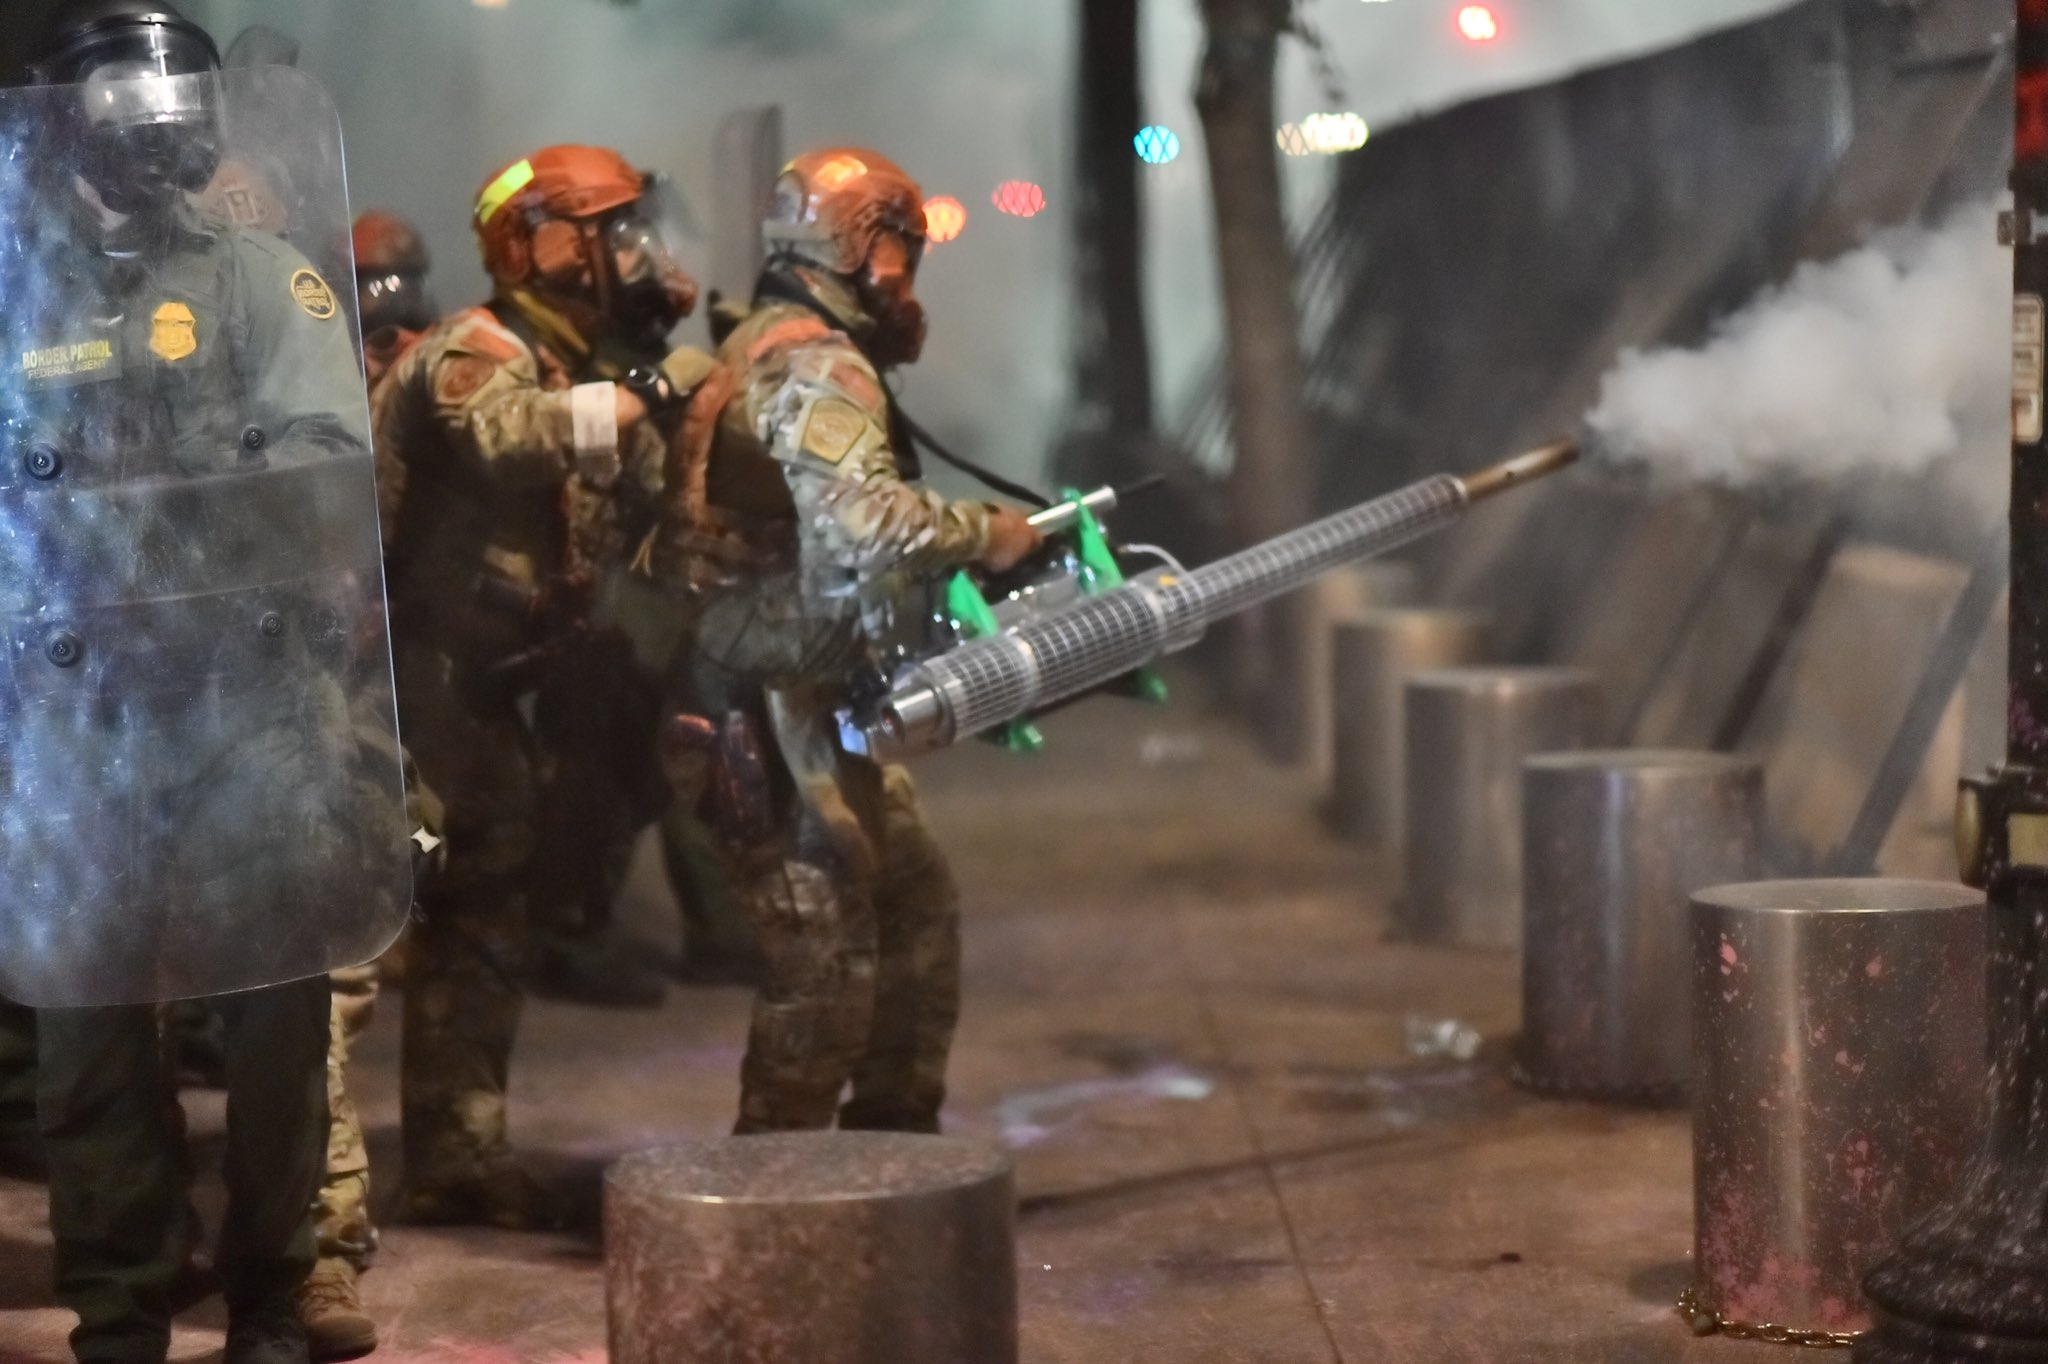
\includegraphics[width=1\linewidth]{img/portland_2020_07_29} 

}

\caption{CBP agent using a thermal fogger in front of the federal courthouse, Portland OR (\protect\hyperlink{ref-Brown2020}{Brown 2020}).}\label{fig:imgportland20200729}
\end{figure}

With this seemingly novel usage, DHS made a large swath of the populace aware of an insidious weapon that is actually not new, but -- in fact -- was \protect\hyperlink{Genesis}{birthed} in the American occupation of Vietnam, \protect\hyperlink{The1968Convensions}{perfected} for use against domestic protesters in the 1960s and '70s, and \protect\hyperlink{CBP}{sent abroad} via CBP in the years since.
The subsequent \protect\hyperlink{PortlandOR2020_2021}{return} of the thermal fogger to use against civilians domestically by the same domestic law enforcement agency (CBP) that sent it abroad after its initial domestic use is an extension of the classical Imperialist Boomerang (\protect\hyperlink{ref-Cesaire1950}{Césaire 1950}, \protect\hyperlink{ref-Arendt1951}{Arendt 1951}, \protect\hyperlink{ref-Foucault1976}{Foucault 1976}, \protect\hyperlink{ref-Graham2013}{Graham 2013}) that can be more aptly described as a tetherball.

Despite repeated use of thermal foggers to deploy chemical weapons over the last half century, the device appears to have slipped from the zeitgeist, only to reemerge in the city that experienced the most visible federal deployment of chemical weapons (\protect\hyperlink{ref-Flanigan2020}{Flanigan 2020}) and weapons-based incidents of police brutality at racial justice protests (regardless of population size) (\protect\hyperlink{ref-pb20202021}{PB2020 Team 2021}), perhaps due to the noteworthy density of photographers and videographers.

Although not all of the weapon's history is documented, enough is that we can quickly dispel the myth that this deployment was \emph{new} in any notable sense other than being recent.

\hypertarget{Science}{%
\section{The Science of Thermal Fogging}\label{Science}}

Broadly speaking, a fog is a visible aerosol that hangs in the air near the ground, and while it occurs on its own accord, humans have devised a variety of methods to generate fog.
And many, if not all, of those methods have been used to deploy chemical weapons on people.
The focus of this book is on \textbf{thermal} fogging.
The idea behind thermal fogging is the same whether you're targeting mosquitoes in a marsh or protesters on a street: flash-vaporize a liquid being forced into a stream of cooler air, causing a fog to form as it condenses; move to increase the size of the cloud.

The original chemical weapons thermal foggers employed the exhaust lines of diesel trucks or manifolds of 2-cycle engines to heat the formulation, which worked but were bulky and difficult to control in open areas (\protect\hyperlink{ref-Crockett1969}{Crockett 1969}).
These models were quickly supplanted by foggers leveraging resonant \href{https://en.wikipedia.org/wiki/Pulsejet}{pulsejet technology} that were streamlined, lighter, and gave control of the stream to the operator (\protect\hyperlink{ref-Applegate1969}{Applegate 1969})



\begin{figure}

{\centering 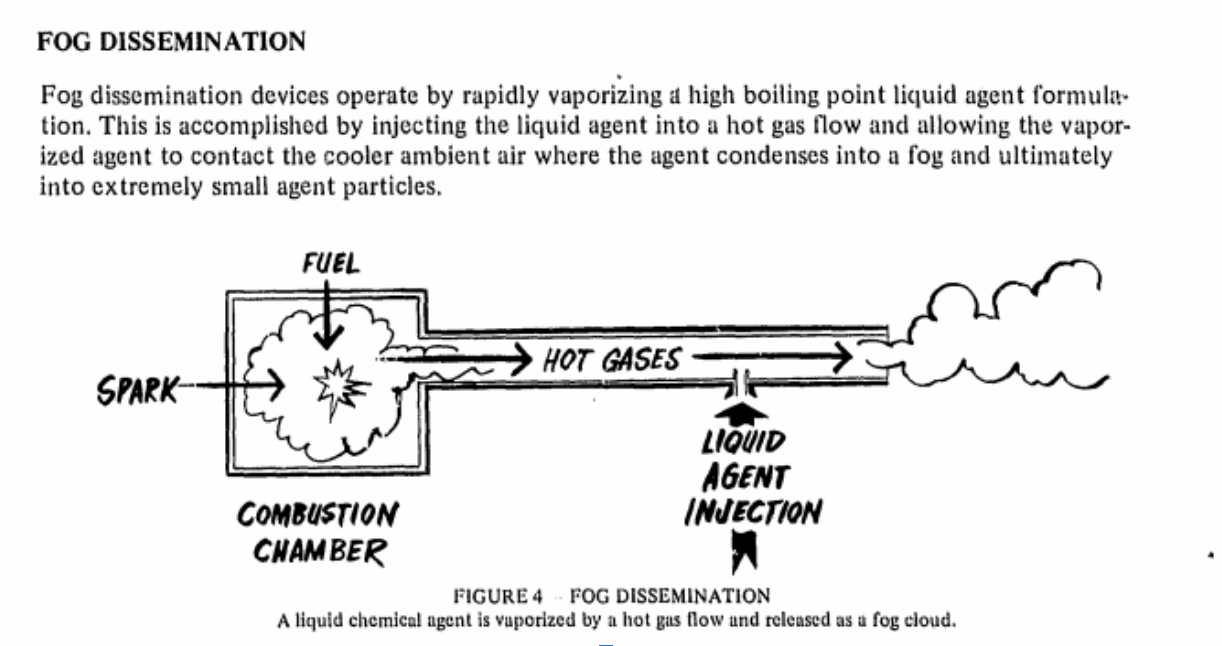
\includegraphics[width=1\linewidth]{img/Crockett1969} 

}

\caption{Concept drawing from the International Association of Chiefs of Police chemical agents manual (\protect\hyperlink{ref-Crockett1969}{Crockett 1969}).}\label{fig:imgCrockett1969}
\end{figure}

Regardless of the heating method specifics, the machine creates a visible fog from the mixture of gasoline exhaust, chemical weapons, and ambient air moisture, as desired.

Although the mixture does cool considerably from its peak temperature before being released, the chemicals are heated to such high temperatures that they thermally decompose, creating a much more toxic mixture of gases that condense to form the fog.
Indeed, the thermal cracking temperatures of common chemical contemporary chemical weapons are well below the temperatures achieved in a thermal fogger:

\begin{itemize}
\tightlist
\item
  Phenacyl chloride (CN): 248 C (\protect\hyperlink{ref-Compton1987}{Compton 1987})
\item
  2-chlorobenzalmalononitrile (CS): 450 - 550 C (\protect\hyperlink{ref-Xueetal2015}{Xue et al. 2015})
\item
  Oleoresin Capsicum (OC): \textless{} 200 C (\protect\hyperlink{ref-HendersonandHenderson1992}{Henderson and Henderson 1992})
\item
  Hexachloroethane (HC): 185 C (\protect\hyperlink{ref-IARC1979}{IARC 1979})
\item
  Terephthalic Acid (TPA): 445 C (\protect\hyperlink{ref-KimyonokandUluturk2016}{Kimyonok and Ulutürk 2016})
\end{itemize}

As a result, it is impossible for anyone to definitively know what chemicals they are fogging someone with, but it is fair to say the mixtures are likely to have considerably higher toxicities than product labels and safety sheets indicate, which are already concerning (\protect\hyperlink{ref-defteccs}{Defense Technology 2015}).

\hypertarget{Vietnam}{%
\chapter{Vietnam}\label{Vietnam}}

The modern day use of thermal foggers for chemical weapons deployment was born from the American colonization of Vietnam in the mid-to-late-20th Century (\protect\hyperlink{ref-USMACV1965}{USMACV 1965}, \protect\hyperlink{ref-Bunker1996}{Bunker 1996}).



\begin{figure}

{\centering 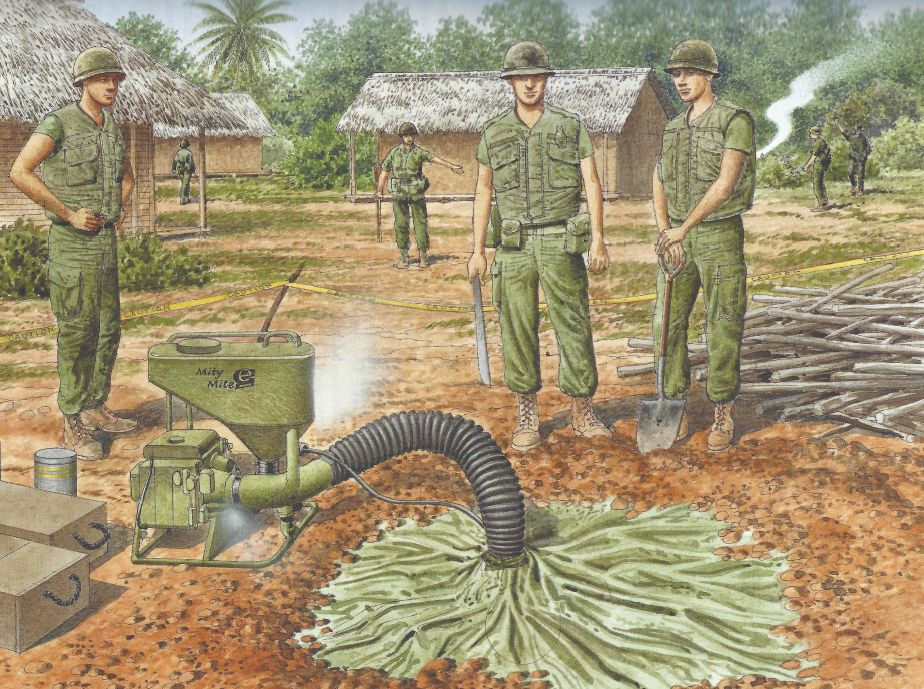
\includegraphics[width=1\linewidth]{img/vcmm} 

}

\caption{US Military deploying a thermal fogger into a Vietnamese tunnel (\protect\hyperlink{ref-Delf2012}{Delf 2012}).}\label{fig:imgvcmm}
\end{figure}

\hypertarget{context}{%
\section{Context}\label{context}}

\hypertarget{mosquito-control}{%
\subsection{Mosquito Control}\label{mosquito-control}}

Early in the deployment of US troops to occupy Vietnam, the need for large scale mosquito control became so great that soldiers began improvising insecticide foggers by piping insecticide into diesel truck exhaust:

\begin{quote}
An insecticide fogger, one of the most useful improvisations, was made by mounting a {[}55-gallon oil{]} drum filled with 6 to 7 percent malathion insecticide in diesel oil \ldots{} on a 3/4-ton truck and spraying the poisonous mixture out with the exhaust from the vehicle. The insecticide is drawn from the drum by the partial vacuum in a line connected to the exhaust pipe just behind the manifold, and sprayed out under pressure of the exhaust.

\VA{--- \protect\hyperlink{ref-Spicknall1969}{Spicknall} (\protect\hyperlink{ref-Spicknall1969}{1969})}{}
\end{quote}

The hack turned out to be \textbf{\emph{4,500 times}} more effective, covering nine square miles per day compared to 50,000 square feet (0.002 square miles) per day using a conventional manually operated fogger (\protect\hyperlink{ref-Spicknall1969}{Spicknall 1969}).
Given widespread mosquito concerns and the preponderance on diesel drums, the truck approach spread, and the concept of fogging was understood among servicemembers (\protect\hyperlink{ref-USMACV1965}{USMACV 1965}, \protect\hyperlink{ref-Spicknall1969}{Spicknall 1969}).

\hypertarget{tunnels}{%
\subsection{Tunnels}\label{tunnels}}

As the occupation continued, underground bunkers and tunnels dug by the Viet Cong (VC) and People's Army of Vietnam (PAV) became a dominant presence on the both the literal and figurative battlefields (\protect\hyperlink{ref-Rottman2006}{Rottman 2006}, \protect\hyperlink{ref-Rottman2012}{2012}).



\begin{figure}

{\centering 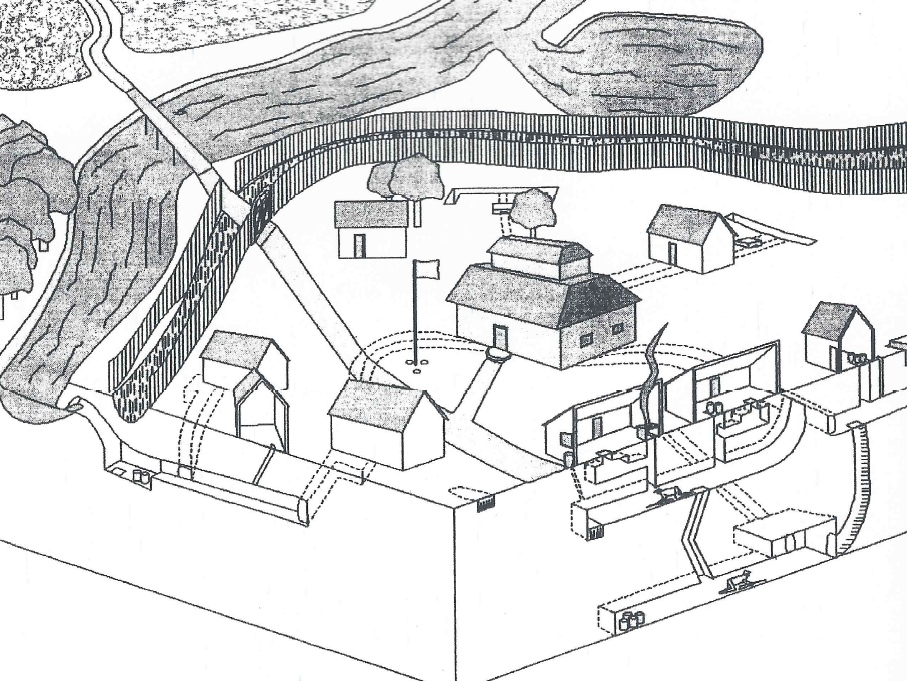
\includegraphics[width=1\linewidth]{img/tunnels} 

}

\caption{Hypothetical Vietnamese village with a two-level bunker tunnel system (\protect\hyperlink{ref-Hanesalo1996}{Hanesalo 1996}).}\label{fig:imgtunnels}
\end{figure}

Soldiers from the US, Australian, New Zealand, and other armies were tasked with clearing the tunnels and ``rooting out'' inhabitants (\protect\hyperlink{ref-Hemmings2019}{Hemmings 2019}).
The specialized forces designated for the work were dubbed ``Tunnel Rats'' and tear gas was part of their arsenal to ``flush'' individuals from caves, which they regularly deployed via pyrotechnic grenades and powdered explosives (\protect\hyperlink{ref-NewYorkTimes1977}{Faas 1977}, \protect\hyperlink{ref-Rottman2006}{Rottman 2006}).



\begin{figure}

{\centering 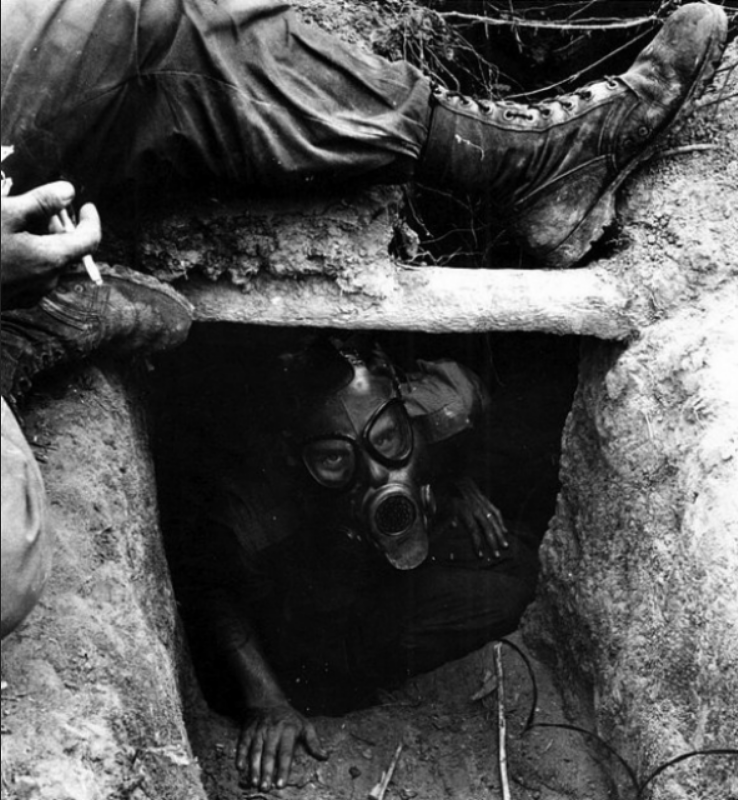
\includegraphics[width=1\linewidth]{img/rat_mask} 

}

\caption{Tunnel rat in a gas mask, undated (\protect\hyperlink{ref-Hemmings2019}{Hemmings 2019})}\label{fig:imgratmask}
\end{figure}

\hypertarget{Genesis}{%
\section{Genesis}\label{Genesis}}

\hypertarget{FirstUse}{%
\subsection{Implementation}\label{FirstUse}}

In October of 1965, the USMACV (United States Military Assistance Command, Vietnam) was supporting the South Vietnamese Army's (ARVN) III Corps in a ``search and destroy'' operation in the Iron Triangle, an area known to house an elaborate Viet Cong tunnel system (\protect\hyperlink{ref-USMACV1965}{USMACV 1965}).



\begin{figure}

{\centering 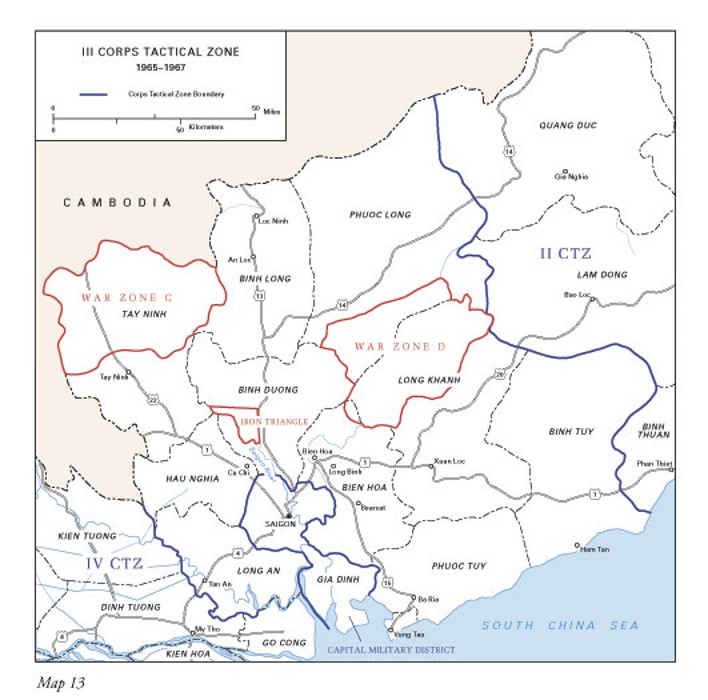
\includegraphics[width=1\linewidth]{img/iron_triangle} 

}

\caption{US-defined War Zones C, D, and the Iron Triangle near Saigon, Vietnam (\protect\hyperlink{ref-USArmy2005}{US Army 2005})}\label{fig:imgirontriangle}
\end{figure}

The US Chemical Advisor to the ARVN's Chemical Team participated in planning the operation, and suggested using a Mity Mite (a.k.a. Mitey Mite, Mighty Mite) 2-cycle thermal fogger to aid in clearing tunnels.
A 6-member unit of ARVN Chemical Team members was organized on October 7th for implementation of the fogger (\protect\hyperlink{ref-USMACV1965}{USMACV 1965}).
The next day, the force located a tunnel and set into motion an elaborate scheme to fog the tunnels with \href{https://chemicalweaponsresearch.com/hc}{hexachloroethane (HC)} smoke from burning pots, marking the first known tactical use of a thermal fogger to deploy chemical weapons agents (\protect\hyperlink{ref-USMACV1965}{USMACV 1965}, \protect\hyperlink{ref-Rottman2012}{Rottman 2012}).
Overall, the endeavor was dubbed a success, despite the tunnel already being empty (\protect\hyperlink{ref-USMACV1965}{USMACV 1965}).

Although (highly toxic; \protect\hyperlink{ref-Simonis2020}{Simonis} (\protect\hyperlink{ref-Simonis2020}{2020})) munitions smoke was used in this application, it was noted that tear gas would be ``very effective in flushing VC from tunnels'' should there been any present (\protect\hyperlink{ref-USMACV1965}{USMACV 1965}).

According to the \emph{Lessons Learned} report filed by the USMACV the next month,

\begin{quote}
This is believed to have been the first tactical employment of Mity Mite \emph{by ARVN}. {[}emphasis added{]}

\VA{--- \protect\hyperlink{ref-USMACV1965}{USMACV} (\protect\hyperlink{ref-USMACV1965}{1965})}{}
\end{quote}

Note that there is no mention of use by USMACV prior to this deployment (\protect\hyperlink{ref-USMACV1965}{USMACV 1965}).

\hypertarget{what-about-not-in-tunnels}{%
\subsection{What About Not In Tunnels?}\label{what-about-not-in-tunnels}}

Seeing the Mity Mite in action got the wheels turning in the heads of USMACV officers, and the idea of deploying the fogger outside of tunnels was on the table (\protect\hyperlink{ref-USMACV1965}{USMACV 1965}).

This is made clear in the \emph{Lessons Learned} report, where they state that the

\begin{quote}
Mity Mite portable blower can be used to \ldots{} generate an agent cloud for use against unmasked personnel \textbf{in the open} \ldots{} {[}emphasis added{]}

\VA{--- \protect\hyperlink{ref-USMACV1965}{USMACV} (\protect\hyperlink{ref-USMACV1965}{1965}).}{}
\end{quote}

At the time, however, the set up used powder, pot, and grenade sources of chemical agents, which was inefficient and required extensive supplies and gasoline reserves (\protect\hyperlink{ref-USMACV1965}{USMACV 1965}).



\begin{figure}

{\centering 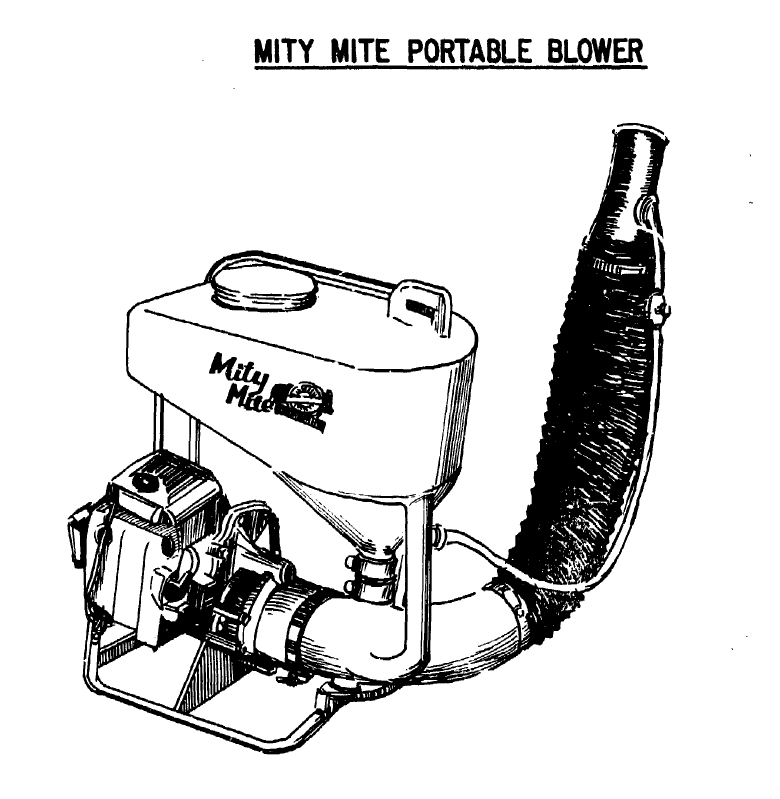
\includegraphics[width=1\linewidth]{img/mity_mite} 

}

\caption{Technical drawing of a backpack fogger (\protect\hyperlink{ref-USMACV1965}{USMACV 1965})}\label{fig:imgmitymite}
\end{figure}

\hypertarget{expansion}{%
\section{Expansion}\label{expansion}}

The practice caught on quickly, and Mity Mites were soon issued to ARVN units (\protect\hyperlink{ref-USMACV1965}{USMACV 1965}) and became common tools for Tunnel Rats (\protect\hyperlink{ref-Rottman2012}{Rottman 2012}).



\begin{figure}

{\centering 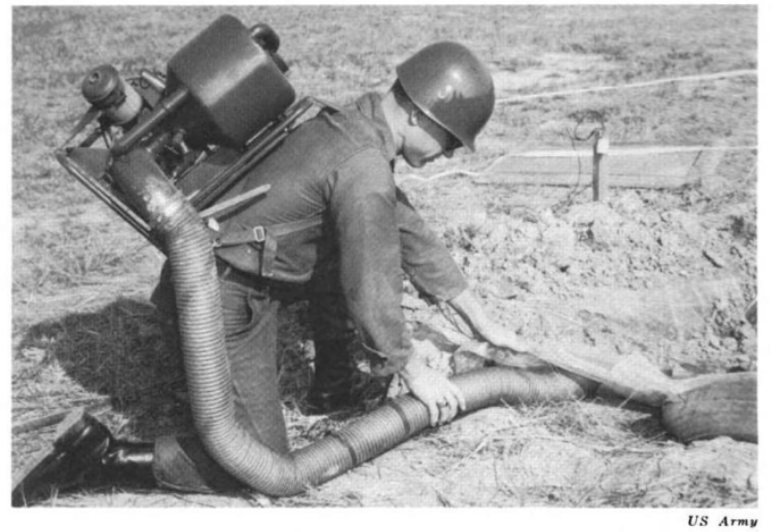
\includegraphics[width=1\linewidth]{img/mighty_mite} 

}

\caption{A soldier uses a backpack Mity Mite to fog a tunnel (\protect\hyperlink{ref-USArmy1966}{US Army 1966})}\label{fig:imgmightymite}
\end{figure}

The Army used foggers to pump ``air'' or ``smoke'' into tunnels in combination with ``riot control agents'' during Operation Cedar falls in 1967 (\protect\hyperlink{ref-Lehrer1968}{Lehrer 1968}).
And by 1968's Battle of Khe Sanh, it was standard practice to use foggers for tunnel excavation as well as mosquito and fly control (\protect\hyperlink{ref-Rottman2006}{Rottman 2006}).



\begin{figure}

{\centering 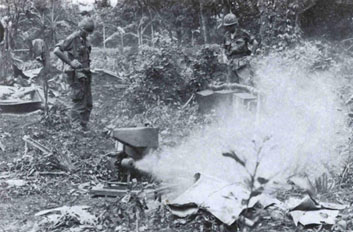
\includegraphics[width=1\linewidth]{img/unpack_test} 

}

\caption{Engineers unpack and test a Mitey-Mite blower (\protect\hyperlink{ref-USAES}{School 2003}).}\label{fig:imgunpacktest}
\end{figure}

In 1969, the US Army Limited War Laboratory published a report on chemical weapons that included a section on foggers and agents for use in them, naming the \protect\hyperlink{GOEC}{General Ordinance Equipment Corporation} and \protect\hyperlink{DefenseTech}{Federal Laboratories} models that were already in production and a propsed development of a formalized truck-based fogger (\protect\hyperlink{ref-Samuelsetal1969}{Samuels et al. 1969}):



\begin{figure}

{\centering 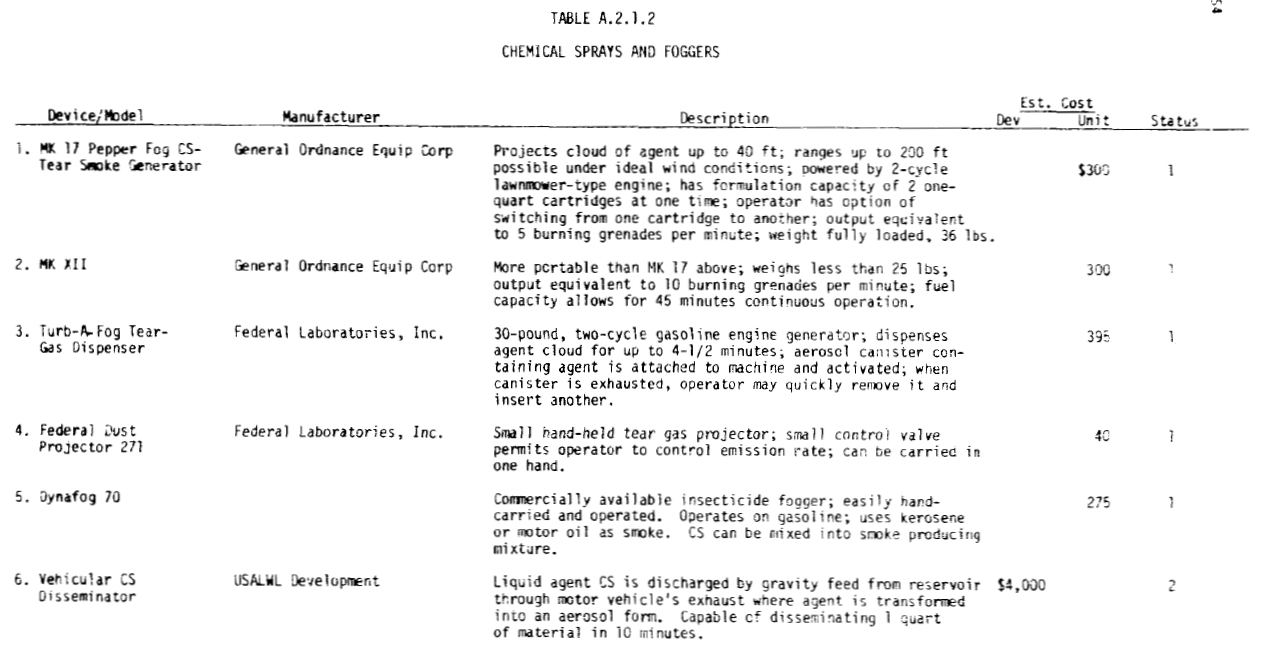
\includegraphics[width=1\linewidth]{img/tablea212} 

}

\caption{Existing and proposed fogging devices (\protect\hyperlink{ref-Samuelsetal1969}{Samuels et al. 1969}).}\label{fig:imgtablea212}
\end{figure}

\hypertarget{international-melting-pot}{%
\section{International Melting Pot}\label{international-melting-pot}}

Other countries explicitly supported the US colonization in Vietnam, providing a pathway for the fogger to be rapidly picked up by the armed forces of other nations.

By 1966 the Australian Tunnel Rats were particularly fond of fogging tunnels with acetylene (\protect\hyperlink{ref-vietnam_aus1}{MacGregor 1966a}, \protect\hyperlink{ref-vietnam_aus2}{1966b}).



\begin{figure}

{\centering 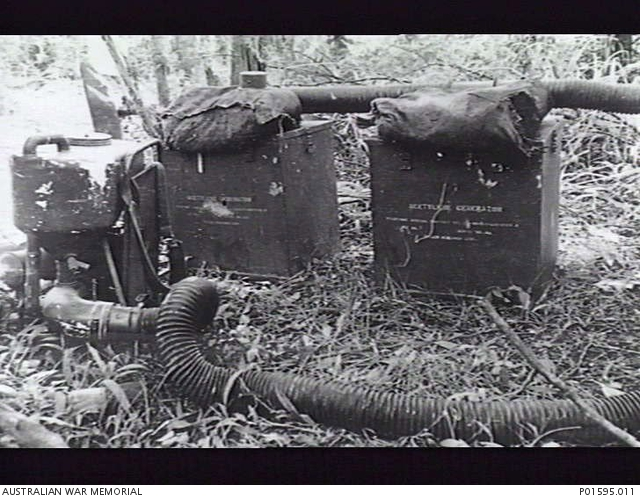
\includegraphics[width=1\linewidth]{img/vietnam_aus1} 

}

\caption{Double Acetylene Generator and a Mighty Mite Air Blower Used to Blow Fumes into Viet Cong Tunnels (\protect\hyperlink{ref-vietnam_aus1}{MacGregor 1966a})}\label{fig:vietnamaus1}
\end{figure}



\begin{figure}

{\centering 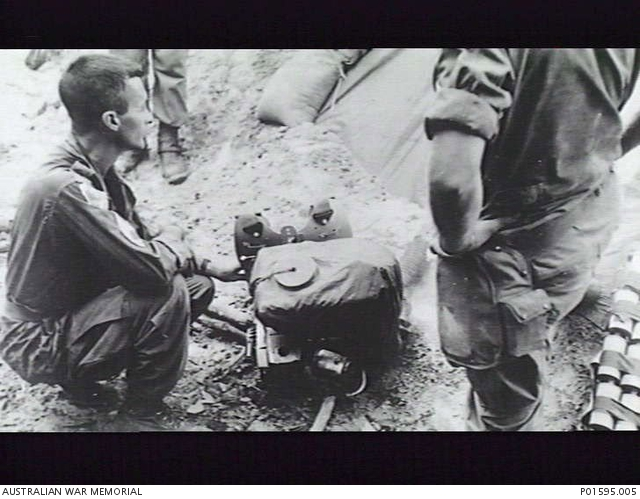
\includegraphics[width=1\linewidth]{img/vietnam_aus2} 

}

\caption{Mighty Mite Machine Used to Contaminate Viet Cong Tunnel Systems with Acetylene (\protect\hyperlink{ref-vietnam_aus2}{MacGregor 1966b})}\label{fig:imgvietnamaus2}
\end{figure}

\protect\hyperlink{TheReturn}{As expected}, the fogger quickly made it to Australian police departments, although with a decidedly negative response from the news media, who called it ``highly controversial'' admist a Sydney Police spending scandal (\protect\hyperlink{ref-Allen1972}{Allen 1972}).
Unnamed Australian arms experts who spoke on background said there was no application for the fogger in the country (\protect\hyperlink{ref-Allen1972}{Allen 1972}), although that hasn't stopped its use elsewhere.

\hypertarget{TheReturn}{%
\chapter{The Return}\label{TheReturn}}

As to be expected following the basic trajectory of an Imperial Boomerang (\protect\hyperlink{ref-Cesaire1950}{Césaire 1950}, \protect\hyperlink{ref-Arendt1951}{Arendt 1951}, \protect\hyperlink{ref-Foucault1976}{Foucault 1976}), the repressive technique (thermal fogging) developed by an imperialist country (USA) to control colonial territories (Vietnam) was brought home by the imperialist nation to use on its own people (\protect\hyperlink{ref-Graham2013}{Graham 2013}).

Indeed, it took just \emph{three years} from initial deployment \protect\hyperlink{FirstUse}{in Vietnam on October 8 1965} to first application in the United States to gas Black racial justice protesters in \protect\hyperlink{MiamiFL1968_08_08}{Miami, Florida on August 8th, 1968} during the Liberty City Riots (\protect\hyperlink{ref-Tschenschlok1995}{Tschenschlok 1995}, \protect\hyperlink{ref-Lorentzen2018}{Lorentze 2018}).

In alignment with the general ``Imperial Circuit of Tear Gas'' (\protect\hyperlink{ref-Schrader2019}{Schrader 2019}) between the US and Vietnam, the return of the fogger was aided significantly by the weapons industry, militarization of US police forces, transition of veterans to law enforcement upon returning home, and substantial propaganda in specialized and generalized outlets.

\hypertarget{manufacturers}{%
\section{Manufacturers}\label{manufacturers}}

American companies quickly jumped at the opportunity to refine the bulky, complicated Mitey Mite and sell thermal foggers to the military and domestic police departments.
As early as 1969, The International Association of Chiefs of Police included a detailed section on thermal fogging and available models in their Chemical Agents Manual (\protect\hyperlink{ref-Crockett1969}{Crockett 1969}), providing prime trade-focused marketing.
Indeed, both \protect\hyperlink{FederalLaboratories}{Federal Laboratories} and \protect\hyperlink{GOEC}{General Ordnance Equipment Corporation} models were included.

\hypertarget{sears-roebuck}{%
\subsection{Sears Roebuck}\label{sears-roebuck}}

The original Mighty Mite that \protect\hyperlink{FirstUse}{established} the fogger as a method of chemical dispersal was manufactured by Sears, Roebuck, and Co.~for insecticide application (\protect\hyperlink{ref-Applegate1969}{Applegate 1969}).



\begin{figure}

{\centering 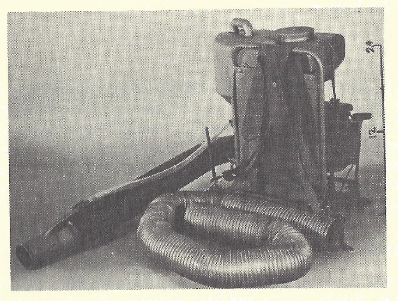
\includegraphics[width=1\linewidth]{img/M106} 

}

\caption{M-106 Mity Mite Thermal Fogger, as promoted to law enforcement in \protect\hyperlink{ref-Applegate1969}{Applegate} (\protect\hyperlink{ref-Applegate1969}{1969}).}\label{fig:imgM106}
\end{figure}

The bulkiness of the Mity Mite backpack proved to be a hindrance in mobile application, however, and while chemical weapons corporations began their fogger lines with hand-held models using 2-cycle engines, there was a push to produce a more streamlined and specialized tool for fogging chemical weapons at civilians (\protect\hyperlink{ref-Applegate1969}{Applegate 1969}, \protect\hyperlink{ref-Applegate1970}{1970}).



\begin{figure}

{\centering 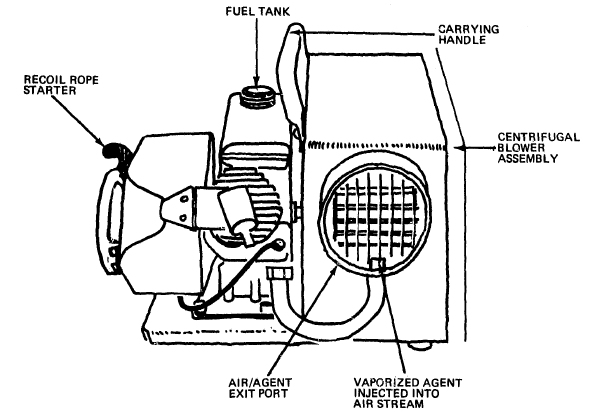
\includegraphics[width=1\linewidth]{img/jetfogger} 

}

\caption{Hand-held two-cycle thermal fogger (\protect\hyperlink{ref-Crockett1969}{Crockett 1969}).}\label{fig:imgjetfogger}
\end{figure}

Sears does not appear to have entered The Mity Mite into the law enforcement market, perhaps due to the company's existing legacy branding, and the model never established itself in the domestic market.

\hypertarget{FederalLaboratories}{%
\subsection{Federal Laboratories}\label{FederalLaboratories}}

Federal Laboratories, one of the major US manufacturers of chemical weapons starting after World War I, developed a hand-held 2-cycle thermal fogger that did not need a backpack or hoses:



\begin{figure}

{\centering 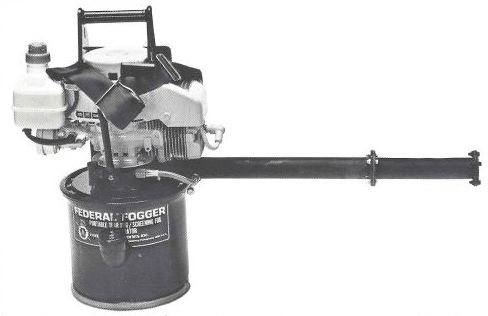
\includegraphics[width=0.75\linewidth]{img/federal_fogger_crop} 

}

\caption{The Federal Laboratories ``Federal Fogger 298'' (\protect\hyperlink{ref-FedLabs298}{Federal Laboratories 1980}).}\label{fig:img298}
\end{figure}



\begin{figure}

{\centering 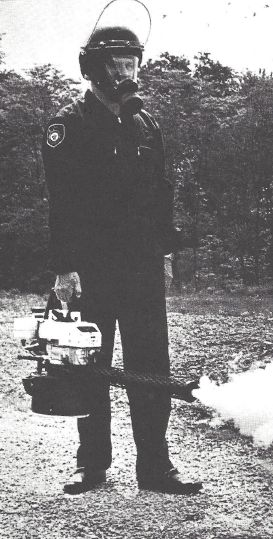
\includegraphics[width=0.75\linewidth]{img/federal_labs} 

}

\caption{Officer demonstrating the Federal Laboratories 298 (\protect\hyperlink{ref-Applegate1992}{Applegate 1992}).}\label{fig:fedlabimg}
\end{figure}

\hypertarget{GOEC}{%
\subsection{General Ordnance Equipment Corporation}\label{GOEC}}

The General Ordnance Equipment Corporation (GOEC), who invented and trademarked Chemical Mace earlier in the decade, had been bought-out by Smith and Wesson by the late 1960s when the fogger market opened up (\protect\hyperlink{ref-Gross2014}{Gross 2014}).

Alan Litman, the brains behind GOEC, retained leadership of chemical weapons development after the buy-out, however (\protect\hyperlink{ref-Gross2014}{Gross 2014}), and he must have seen an opportunity, as GOEC began selling hand-held thermal foggers in July 1968 (\protect\hyperlink{ref-Applegate1969}{Applegate 1969}).

They named their units ``Pepper Fog'' generators, a nod to their apparent ability to ``pepper'' the recipient with more concentrated bursts of fog if desired, compared to the steady stream output from the Mity Mite (\protect\hyperlink{ref-Applegate1969}{Applegate 1969}), and applied for a trademark on the phrase in October of the same year (\protect\hyperlink{ref-USTPO2018}{USTPO 2018}).
By the end of August 1969, GOEC (and thus Smith and Wesson) had received the trademark on ``Pepper Fog,'' which they (and subsequent owners) retained until it expired in 1991 (\protect\hyperlink{ref-USTPO2018}{USTPO 2018}).

While GOEC did develop and sell a stationary 2-cycle model for vehicle mounting, it was their hand-held pulse-jet model that took the market by storm (\protect\hyperlink{ref-Crockett1969}{Crockett 1969}).



\begin{figure}

{\centering 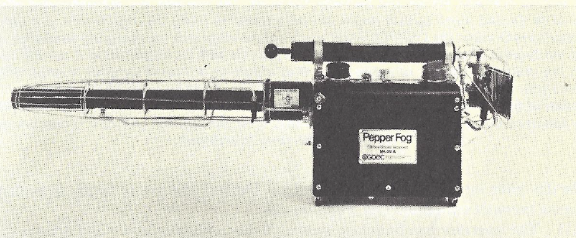
\includegraphics[width=1\linewidth]{img/goec_pf} 

}

\caption{General Ordnance Equipment Corporation thermal fogger (\protect\hyperlink{ref-GOECphoto}{General Ordnance Equipment Corporation 1969a}), as shown in \protect\hyperlink{ref-Applegate1969}{Applegate} (\protect\hyperlink{ref-Applegate1969}{1969}).}\label{fig:goecpf}
\end{figure}

They immediately began a heavy marketing campaign for their new invention, taking out full-page ads in police magazines (\protect\hyperlink{ref-GOECad1969}{General Ordnance Equipment Corporation 1969b}, \protect\hyperlink{ref-GOECadLNS1970}{1969c}, \protect\hyperlink{ref-GOECadObserver1970}{1970}):



\begin{figure}

{\centering 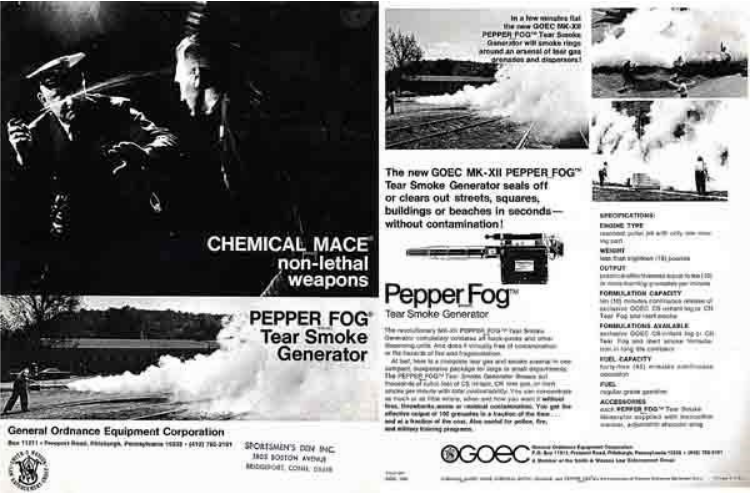
\includegraphics[width=1\linewidth]{img/GOECad1969} 

}

\caption{GOEC advertisement (\protect\hyperlink{ref-GOECad1969}{General Ordnance Equipment Corporation 1969b}).}\label{fig:imggoecad1969}
\end{figure}

They also leveraged the connection between local law enforcement and the press to generate \protect\hyperlink{Propa}{free marketing} with an \protect\hyperlink{Canada}{international reach}.

It is perhaps no surprise then that virtually all of the foggers photographed being used in the US prior to 2020 are GOEC models.

\hypertarget{DefenseTechnology}{%
\subsection{Defense Technology}\label{DefenseTechnology}}

The corporate descendent of both GOEC and Federal Labs and current owner of the legacy branding (\href{https://www.safariland.com}{Safariland} subsidiary \href{https://www.defense-technology.com}{Defense Technology}) continues to sell items under a \href{https://www.defense-technology.com/product-category/pepper-foggers/}{``Pepper Fog'' line}, including a \href{https://www.defense-technology.com/product/pepper-fog-generator/}{``pepper fog generator''} that utilizes the same pulse-jet generation technique (\protect\hyperlink{ref-DTPFG}{Safariland, LLC 2020a}):



\begin{figure}

{\centering 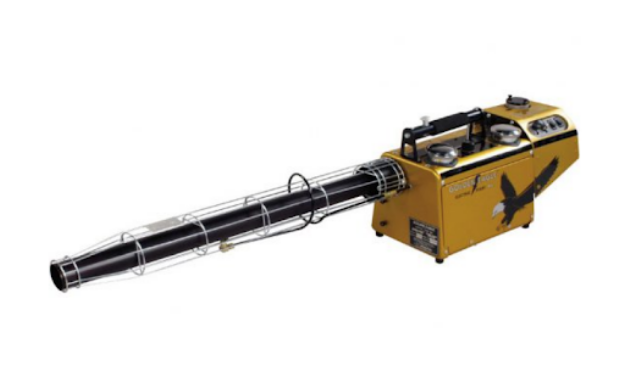
\includegraphics[width=1\linewidth]{img/defense_tech_gepf} 

}

\caption{Product image for thermal fogger (\protect\hyperlink{ref-DTPFGphoto}{Safariland, LLC 2020b}).}\label{fig:imgdefensetechgepf}
\end{figure}

This has supplanted the models produced by the corporate ancestors to Defense Technology, which were bulkier and considerably heavier (\protect\hyperlink{ref-Samuelsetal1969}{Samuels et al. 1969}).

\hypertarget{rex-applegate}{%
\section{Rex Applegate}\label{rex-applegate}}

A major figure in the translation of military ``riot suppression'' tactics to domestic law enforcement in the 1960s and 1970s was a former US Army Lt. Colonel named \href{https://en.wikipedia.org/wiki/Rex_Applegate}{Rex Applegate}.
Applegate took a commission as a second leuitenant, but had a lung ailment kept him from serving in combat in World War II and so was assigned to Military Police Company before being tapped by \href{https://en.wikipedia.org/wiki/William_J._Donovan}{Col. William Donovan} to build and run the School for Spies and Assassins in the Office of Strategic Services (\protect\hyperlink{ref-Goldstein1998}{Goldstein 1998}).
Larger than life, Rex even served as bodyguard to President Franklin Roosevelt, before retiring and moving to Mexico at the end of World War II to consult with Central and South American governments on ``riot control'' (\protect\hyperlink{ref-Goldstein1998}{Goldstein 1998}).

Applegate returned to the US in the 1960s during the civil rights and anti-war protest era and began proselytizing the good word of the thermal fogger (\protect\hyperlink{ref-Applegate1969}{Applegate 1969}, \protect\hyperlink{ref-Applegate1970}{1970}).
Indeed, Rex published what can only be described as a long-form written sales pitch for the GOEC Pepper Fog thermal fogger in the highly circulated \emph{Guns} magazine in 1970 (\protect\hyperlink{ref-Applegate1970}{Applegate 1970}).



\begin{figure}

{\centering 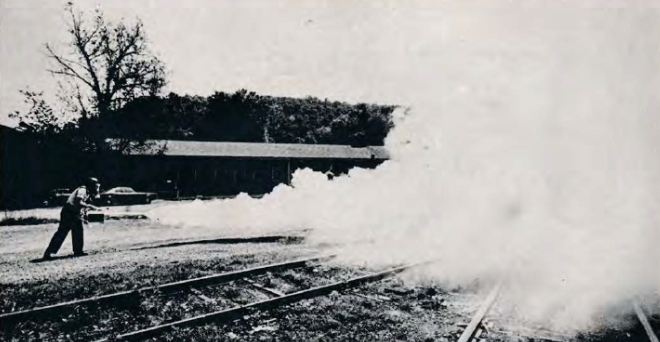
\includegraphics[width=1\linewidth]{img/demo} 

}

\caption{Demonstration of a pepper fogger (\protect\hyperlink{ref-Applegate1970}{Applegate 1970})}\label{fig:imgdemo}
\end{figure}

\hypertarget{Propa}{%
\section{News Media Propaganda}\label{Propa}}

Alongside the more overtly pro-police-use-of-chemical-weapons propaganda of Rex Applegate were other, perhaps more subtle forms of pro-fogger propaganda (\protect\hyperlink{ref-Macomber1970}{Macomber 1970}).
Newspapers around the country were more than happy to print ``articles'' that promoted the new arsenals police departments were building (\protect\hyperlink{ref-LaPrade1970}{LaPrade 1970}), complete with product demo photos.



\begin{figure}

{\centering 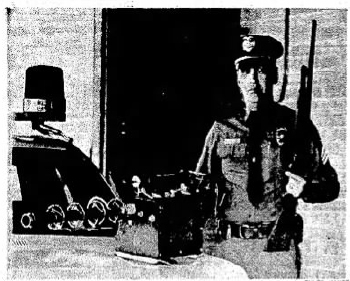
\includegraphics[width=1\linewidth]{img/Vance1970} 

}

\caption{Amarillo Texas Police Sergent Jerry Austin with a thermal fogger and shotgun (\protect\hyperlink{ref-Vance1970}{Vance 1970}). Amarillo's 1970 population was 127,010 (\protect\hyperlink{ref-USCB1970}{USCB 1971}).}\label{fig:imgVance1970}
\end{figure}



\begin{figure}

{\centering 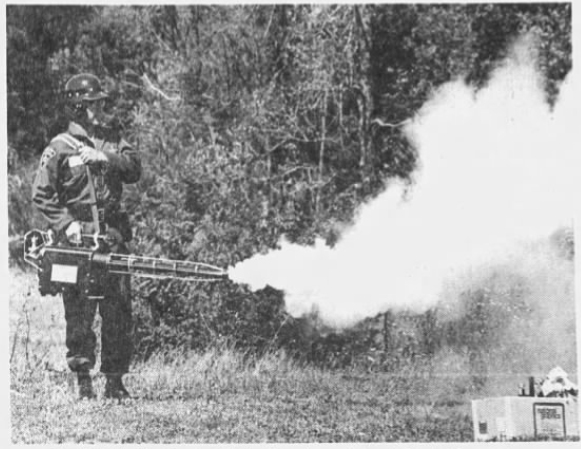
\includegraphics[width=1\linewidth]{img/Amanphoto1970} 

}

\caption{Richland County (Ohio) Sheriff's Captain Robert Dysart demonstrating a thermal fogger to a crowd of \textgreater200 people (\protect\hyperlink{ref-Amanphoto1970}{Aman 1970}). Richland County's 1970 population was 129,997 (\protect\hyperlink{ref-USCB1970}{USCB 1971}).}\label{fig:imgAmanphoto1970}
\end{figure}

\protect\hyperlink{GOEC}{General Ordnance Equipment Corporation}'s Pepper Fog model seems to have been the favorite, at least amongst the departments showing off their new cool toys for photographs.



\begin{figure}

{\centering 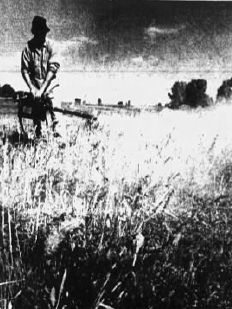
\includegraphics[width=1\linewidth]{img/Gaylord1971} 

}

\caption{A McHenry County (Illinois) Sheriff's officer fogs some grass in a rural landscape during a training and press demo day (\protect\hyperlink{ref-PlainDealer1971}{The McHenry Plaindealer 1971}, \protect\hyperlink{ref-Gaylord1971}{Wayne Gaylord 1971}). McHenry County's 1970 population was 111,555 (\protect\hyperlink{ref-USCB1970}{USCB 1971}).}\label{fig:imgGaylord1971}
\end{figure}



\begin{figure}

{\centering 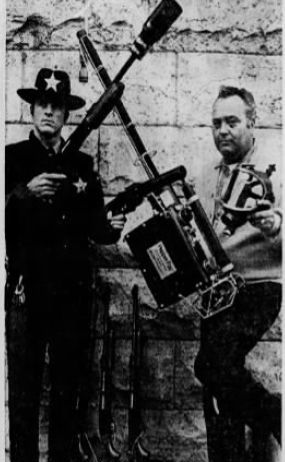
\includegraphics[width=0.75\linewidth]{img/Winter1970} 

}

\caption{Scott County (Iowa) deputy sheriff Jim Lewis, left, holds a new grenade launcher and a riot gun while Sheriff William Strout displays a pepper fogger and gas mask (\protect\hyperlink{ref-Winter1970}{Winter 1970}). Scott County's 1970 population was 142,687 (\protect\hyperlink{ref-USCB1970}{USCB 1971}).}\label{fig:imgWinter1970}
\end{figure}

\hypertarget{gary-wills}{%
\subsection{Gary Wills}\label{gary-wills}}

Pulitzer Prize-winning \href{https://en.wikipedia.org/wiki/Garry_Wills}{Garry Wills} (who at the time was considerably more conservative than he came to be later) penned an op-ed that ran in (at least) The Herald Statesman (Yonkers, New York) (\protect\hyperlink{ref-Wills1971a}{Wills 1971a}), The Daily Item (Port Chester, New York) (\protect\hyperlink{ref-Wills1971b}{Wills 1971b}), The Charlotte News (Charlotte, North Carolina) (\protect\hyperlink{ref-Wills1971c}{Wills 1971c}), and The Philadelphia Inquirer (\protect\hyperlink{ref-Wills1971d}{Wills 1971d}) in April 1971 in which he basically tells all the cry babies (pun intended) to suck it up because he ``would not be afraid to undergo such experiences {[}as being pepper fogged{]} again'' (\protect\hyperlink{ref-Wills1971a}{Wills 1971a}).

Notably, he touts the leading belief at the time that somehow thermal fogging is a ``safe immobilizer of individuals'' (\protect\hyperlink{ref-Wills1971a}{Wills 1971a}), despite the weapon not being demonstrably safer than gas grenades and not only not ``immobilizing'' but explicitly designed to mobilize immobile resisters.
Wills interestingly deems chemical weapons as ``safer than dogs, which get out of control, bite bystanders (and even other cops) as well as `the bad guys'\,'' (\protect\hyperlink{ref-Wills1971a}{Wills 1971a}), despite their being indiscriminate to the point of impacting bystanders, police officers, etc..

He concludes his piece by calling tear gas ``humane in \ldots{} foreign wars {[}and{]} domestic encounters'' (\protect\hyperlink{ref-Wills1971a}{Wills 1971a}), speaking clearly to the return of the trip of the classically defined Imperial Boomerang (\protect\hyperlink{ref-Cesaire1950}{Césaire 1950}, \protect\hyperlink{ref-Arendt1951}{Arendt 1951}, \protect\hyperlink{ref-Foucault1976}{Foucault 1976}).

\hypertarget{The1968Conventions}{%
\chapter{The 1968 National Conventions}\label{The1968Conventions}}

Deployment of chemical weapons on United States civilians by domestic law enforcement began in earnest in the late 1960s during the height of anti-war and civil rights protests, kicked off in particular by the 1968 Republican (Miami, Florida) and Democratic (Chicago, IL) National Conventions (\protect\hyperlink{ref-McArdle2018}{McArdle 2018}, \protect\hyperlink{ref-TaylorandMorris2018}{Taylor and Morris 2018}).
As a result of a \protect\hyperlink{TheReturn}{heavy propaganda and branding campaign}, the thermal fogger was just becoming a mainstay of early police chemical weapons arsenals.
Importantly, by the summer of 1968, the Florida Highway Patrol, Chicago Police Department, and California State Police all had purchased foggers.

Beyond their legacy as the first domestic fogger deployments, the lingering impact of the 1968 Conventions was felt for years to come.
The Kansas City (Missouri) Police Department armed up their chemical weapons cache in advance of the 1976 Republican National Convention, including purchase of fogger fluids (\protect\hyperlink{ref-Hudson1976}{Hudson 1976}).

\hypertarget{republican-national-convention}{%
\section{Republican National Convention}\label{republican-national-convention}}

\hypertarget{MiamiFL1968_08_08}{%
\subsection{Miami, Florida}\label{MiamiFL1968_08_08}}

The first use of a thermal fogger to deploy chemical weapons in the US that I have been able to uncover occured on August 8th 1968, during the ``\href{https://en.wikipedia.org/wiki/1968_Miami_riot}{Liberty City Riots},'' which took place in the midst of the \href{https://en.wikipedia.org/wiki/1968_Republican_National_Convention}{1968 Republican National Convention} (RNC) in Miami, Florida (\protect\hyperlink{ref-Tschenschlok1995}{Tschenschlok 1995}, \protect\hyperlink{ref-Tschenschlok1996}{1996}, \protect\hyperlink{ref-McArdle2018}{McArdle 2018}).
A white reporter with the Miami Herald attempted to gain access to rally of concerned Black people that was meant to be only among Black people that was occurring in Liberty City, a Black neighborhood, on August 7th (\protect\hyperlink{ref-Tschenschlok1995}{Tschenschlok 1995}, \protect\hyperlink{ref-Tschenschlok1996}{1996}).
When the reporter was ejected from the rally, Miami police responded with a large and heavy presence and during the standoff, a white motorist with a ``Wallace for President'' bumper sticker attempted to drive through but was met with resistance and drove into another car, and fled the scene on foot (\protect\hyperlink{ref-Tschenschlok1995}{Tschenschlok 1995}, \protect\hyperlink{ref-Lorentzen2018}{Lorentze 2018}).

Miami police used chemical weapons the night of the 7th, but the fogger did not make an appearance until the subsequent day.
Local, state, and federal officials met with Black organizational representatives the night of the 7th and had agreed to continue discussions the morning of the 8th, but instead sent staffers rather than appear themselves, which effectively ended discussions (\protect\hyperlink{ref-Tschenschlok1995}{Tschenschlok 1995}, \protect\hyperlink{ref-Tschenschlok1996}{1996}).
Apparently, Miami Police Department was unable to manage the situation and Florida Highway Patrol (FHP) was called in by the city (\protect\hyperlink{ref-Tschenschlok1995}{Tschenschlok 1995}).

FHP used a truck with multiple foggers (\protect\hyperlink{ref-Lorentzen2018}{Lorentze 2018}), described as ``essentially a modified version of an insect-control machine'' that ``spread a thick fog of tear gas throughout the riot zone'' (\protect\hyperlink{ref-Tschenschlok1995}{Tschenschlok 1995}).

FHP used the truck-mounted thermal foggers indiscriminately and caused visible symptoms (gagging, etc.) in all present, including a 5-month old (\protect\hyperlink{ref-McArdle2018}{McArdle 2018}).
The fog quickly spread into neighborhood homes, forcing residents outside to seek fresh air (\protect\hyperlink{ref-Tschenschlok1995}{Tschenschlok 1995}).

\hypertarget{democratic-national-convention}{%
\section{Democratic National Convention}\label{democratic-national-convention}}

\hypertarget{ChicagoIL1968_08_26}{%
\subsection{Chicago, Illinois}\label{ChicagoIL1968_08_26}}

Later that month, from August 26th to 29th, anti-war protests took place in Chicago, Illinois during the \href{https://en.wikipedia.org/wiki/1968_Democratic_National_Convention}{Democratic National Convention}, and a massive force of law enforcement (Chicago Police with assistance from over 6,000 National Guard members and 6,000 Army troops (\protect\hyperlink{ref-TaylorandMorris2018}{Taylor and Morris 2018})) responded excessively, including with chemical weapons, on network news (\protect\hyperlink{ref-Schultz1969}{Schultz 1969}, \protect\hyperlink{ref-Karnow1983}{Karnow 1983}, \protect\hyperlink{ref-Farber1988}{Farber 1988}, \protect\hyperlink{ref-Langguth2000}{Langguth 2000}).
After four days, hundreds had been given medical assistance for exposure to chemical weapons (\protect\hyperlink{ref-TaylorandMorris2018}{Taylor and Morris 2018}).

Although I have yet to find contemporary documentation of fogger use during the convention, an AP report on fogger use in \protect\hyperlink{BerkeleyCA1969_02_21}{Berkeley the year later} states

\begin{quote}
A similar device was used during demonstrations in Chicago during the Democratic convention last summer. - \protect\hyperlink{ref-TheDailyTribune1969_02_21}{Associated Press} (\protect\hyperlink{ref-TheDailyTribune1969_02_21}{1969a})
\end{quote}

As such, I consider this a very likely deployment.
I am continuing to search for evidence.

\hypertarget{BerkeleyCA1968_08_31}{%
\subsection{Berkeley, California}\label{BerkeleyCA1968_08_31}}

An August 31st demonstration in Berkeley, California was called by the Young Socialist Alliance, Independent Socialist Club, and the Black Panther Party in solidarity with anti-war protesters in Chicago who the police had recently brutalized (\protect\hyperlink{ref-PatersonEveningNews1968_08_31}{United Press International 1968a}, \protect\hyperlink{ref-TheCapitalTimes1968_08_31}{1968b}), including \protect\hyperlink{ChicagoIL1968_08_26}{use of a pepper fogger} (\protect\hyperlink{ref-TheDailyTribune1969_02_21}{Associated Press 1969a}).
In response, police brutalized the protesters, and in the process brought out a hand-held pepper fogger, a ``new police weapon\ldots{} which produced a gas that caused sneezing'' (\protect\hyperlink{ref-PatersonEveningNews1968_08_31}{United Press International 1968a}).



\begin{figure}

{\centering 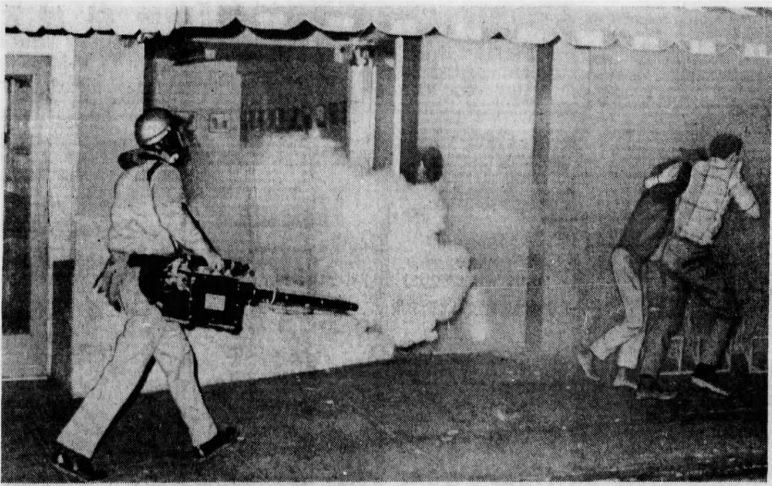
\includegraphics[width=1\linewidth]{img/berkeley_1968_08_31} 

}

\caption{Deployment of a thermal fogger by police in Berkeley, CA (\protect\hyperlink{ref-UPIphoto1968}{United Press International 1968c}).}\label{fig:imgberkeley19680831}
\end{figure}

Deployment of the thermal fogger was covered in newspapers around the country including Paterson, New Jersey (\protect\hyperlink{ref-PatersonEveningNews1968_08_31}{United Press International 1968a}); Hanford, California (\protect\hyperlink{ref-TheHanfordSentinel1968_08_31}{United Press International 1968d}); Honolulu, Hawaii (\protect\hyperlink{ref-TheHonoluluAdvertiser1968_09_01}{United Press International 1968h}); St.~Louis, Missouri (\protect\hyperlink{ref-StLouisPostDispatch1968_08_31}{United Press International 1968e}); Franklin, Pennsylvania (\protect\hyperlink{ref-TheNewsHerald1968_08_31}{United Press International 1968f}); Madison, Wisconsin (\protect\hyperlink{ref-TheCapitalTimes1968_08_31}{United Press International 1968b}); and El Paso, Texas (\protect\hyperlink{ref-ElPasoHeraldPost1968_08_31}{United Press International 1968g}), a city whose significance was already budding.

It is clear from the photograph shared with the United Press International (UPI) copy that the fogger used is a \protect\hyperlink{GOEC}{GOEC} brand pepper fogger, which hit the market the month prior (\protect\hyperlink{ref-USTPO2018}{USTPO 2018}).
The GOEC thermal fogger was so new, it would not have a trademarked name (``Pepper Fog'') for another year (\protect\hyperlink{ref-USTPO2018}{USTPO 2018}).



\begin{figure}

{\centering 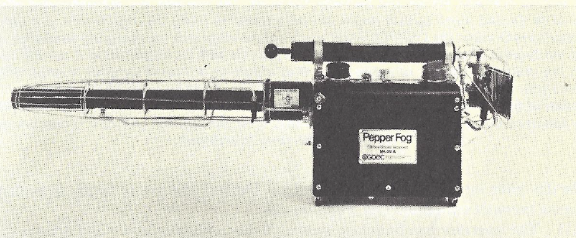
\includegraphics[width=1\linewidth]{img/goec_pf} 

}

\caption{Product image for thermal fogger (\protect\hyperlink{ref-GOECphoto}{General Ordnance Equipment Corporation 1969a}).}\label{fig:imggoecpf}
\end{figure}

\hypertarget{coming-soon-to-a-town-near-you}{%
\chapter{Coming Soon To A Town Near You!}\label{coming-soon-to-a-town-near-you}}

Following the conventions, the fogger quickly became a part of the law enforcement arsenal.
US police had a hard time containing their glee when purchasing and testing thermal foggers for use on domestic civilians, as a general media blitz played out across the country through the late 1960s and early 1970s (\protect\hyperlink{ref-PlainDealer1971}{The McHenry Plaindealer 1971}).

\hypertarget{expansion-from-the-nexuses}{%
\section{Expansion from the Nexuses}\label{expansion-from-the-nexuses}}

\hypertarget{illinois}{%
\subsection{Illinois}\label{illinois}}

In the wake of the \protect\hyperlink{ChicagoIL1968_08_26}{1968 Democratic National Convention}, Chicago-area police played an outsized role in promoting the propaganda line.
The pepper fogger was touted as being able to ``empty a house fast'' by Cook County Illinois Sheriff Joseph Woods (\protect\hyperlink{ref-MtVernonRegisterNews1969_04_09}{Harris 1969b}, \protect\hyperlink{ref-DailyDispatch1969_04_09}{1969c}), a definitely off-spec and dangerous use (\protect\hyperlink{ref-Nixalite2009b}{Nixalite 2009a}).
The volume of fog emitted was also said to be able to fill \href{https://en.wikipedia.org/wiki/Soldier_Field}{Soldier Field (capacity 61,500 fans)} in under a minute (\protect\hyperlink{ref-DailyDispatch1969_04_09}{Harris 1969c}).
Regardless, the Chicago-area Sheriff decided they needed three of them (\protect\hyperlink{ref-DailyDispatch1969_04_09}{Harris 1969c}).
The Sheriff's Major in charge of chemical arsenal Anthony Yucevicius noted the fogger's psychological effect on recipients, as well saying

\begin{quote}
They make a terrifying noise and probably will have a scare effect on crowds.

\VA{--- \protect\hyperlink{ref-TheTerreHauteTribune1969_04_08}{Harris} (\protect\hyperlink{ref-TheTerreHauteTribune1969_04_08}{1969a}).}{}
\end{quote}

Use expanded among and within states, as by 1972 the Illinois State Police also purchased three foggers, which they trained with in Springfield (\protect\hyperlink{ref-Robinson1972}{Robinson 1972}).
In news reports, the foggers were described as

\begin{quote}
a cross between a machine gun, a power lawn mower, and a sun lamp.

\VA{--- \protect\hyperlink{ref-Robinson1972}{Robinson} (\protect\hyperlink{ref-Robinson1972}{1972}).}{}
\end{quote}

\hypertarget{florida}{%
\subsection{Florida}\label{florida}}

Similarly, following the \protect\hyperlink{MiamiFL1968_08_08}{1968 Republican National Convention}, Florida law enforcement took to the fogger (\protect\hyperlink{ref-Cain1968}{Cain 1968}).
In Sanford (1970 pop. 17,393; \protect\hyperlink{ref-USCB1970}{USCB} (\protect\hyperlink{ref-USCB1970}{1971})), the local police department purchased a fogger for use with \href{https://en.wikipedia.org/wiki/Phenacyl_chloride}{CN gas}, noting that it could shoot fog 20 ft for up to a 15 minute stretch, and so would be effective for controlling large masses (\protect\hyperlink{ref-Cain1968}{Cain 1968}).
They had, however, only used it in training and for demoing to the media (\protect\hyperlink{ref-Cain1968}{Cain 1968}).



\begin{figure}

{\centering 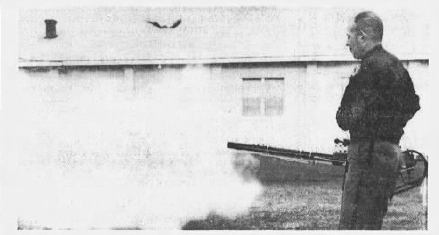
\includegraphics[width=1\linewidth]{img/OrlandoEveningStar1968} 

}

\caption{Sanford Police Officer Roy Williams shows off a fogger (\protect\hyperlink{ref-OrlandoEveningStar1968}{Orlando Evening Star 1968}).}\label{fig:imgOrlandoEveningStar1968}
\end{figure}

\hypertarget{california}{%
\subsection{California}\label{california}}

Eager to not be shown up by the police in Berkeley, by 1970, the Los Angeles Sheriff's Department had already purchased their own fogger for their ``big artillery'' to use ``when other forms of persuasion have failed'' and started a media campaign (\protect\hyperlink{ref-Michals1970}{Michals 1970}).
The department and new state regulations required officers to be trained in chemical weapons use, which was set up through Officer Robert Hawkins (\protect\hyperlink{ref-Michals1970}{Michals 1970}).



\begin{figure}

{\centering 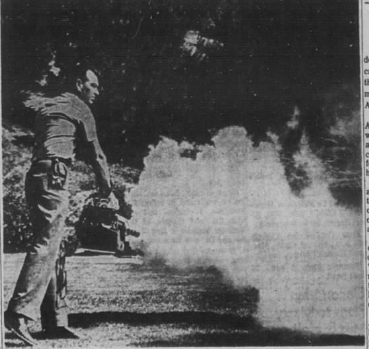
\includegraphics[width=1\linewidth]{img/CopleyNewsService1970} 

}

\caption{Los Angeles Sheriff's Department Officer demonstrating a fogger (\protect\hyperlink{ref-CopleyNewsService1970}{Copley News Service 1970}).}\label{fig:imgCopleyNewsService1970}
\end{figure}

\hypertarget{national-guard}{%
\section{National Guard}\label{national-guard}}

Following the Kent State Massacre, the Ohio National Guard, as well as others around the country began equipping their forces with thermal foggers, using the death of those students as justification for massive purchaing of ``less lethal'' options (\protect\hyperlink{ref-Bandy1970}{Bandy 1970}).

\hypertarget{small-town-usa}{%
\section{Small Town USA}\label{small-town-usa}}

No matter the size of the town, by the early 70s, police wanted in on that sweet sweet fogger action.
The Brigham City (Utah; 1970 pop. 14,007; \protect\hyperlink{ref-USCB1970}{USCB} (\protect\hyperlink{ref-USCB1970}{1971})) Police Department leveraged federal Omnibus Crime Act money to purchase a variety of weapons to use against protesters in 1971 (\protect\hyperlink{ref-BoxElderAgencies1971}{Box Elder Agencies 1971}).

Police Chief Jay Christensen noted that the fogger provides a longer shelf-life than grenades and reportage noted that it

\begin{quote}
emits a continuous stream of smoke, chemical irritants, or \textbf{whatever solution} is fed into it. {[}emphasis added{]}

\VA{--- \protect\hyperlink{ref-Robinson1972}{Robinson} (\protect\hyperlink{ref-Robinson1972}{1972})}{}
\end{quote}

Use of federal funds to purchase chemical weapons, and specifically foggers, was not limited to one department.
Cities, counties, and states across the country used Omnibus Crime Bill money to up their chemical weapons caches, including foggers (\protect\hyperlink{ref-Conheim1972}{Conheim 1972}).
For example, Oakland County in Michigan (1970 pop. 907,871; \protect\hyperlink{ref-USCB1970}{USCB} (\protect\hyperlink{ref-USCB1970}{1971})) purchased two pepper foggers for their South County Tactical Mobile Unit with part of their \$21,066 in 1970 (\protect\hyperlink{ref-Conheim1972}{Conheim 1972}).

Oneota New York (1970 pop. 16,030; \protect\hyperlink{ref-USCB1970}{USCB} (\protect\hyperlink{ref-USCB1970}{1971})) purchased a fogger in 1969 during the anti-war demonstrations, although the department bungled its response to protests (\protect\hyperlink{ref-Griffin1973}{Griffin 1973}).
As came to light during a public probe, Oneota Police Chief Joseph F. DeSalvatore requested a limited amount of training in the budget, and officers were therefore unable to deploy the fogger or other chemical weapons (\protect\hyperlink{ref-Griffin1973}{Griffin 1973}).

Gaston County North Caolina (1970 pop. 47,322; \protect\hyperlink{ref-USCB1970}{USCB} (\protect\hyperlink{ref-USCB1970}{1971})) Sheriffs purchased a fogger, which they turned on but not used to dispense agents multiple times by 1970 in their jail system ``when there's been trouble brewing'' (\protect\hyperlink{ref-Balloch1970}{The Gastonian Gazette Sun 1970a}).



\begin{figure}

{\centering 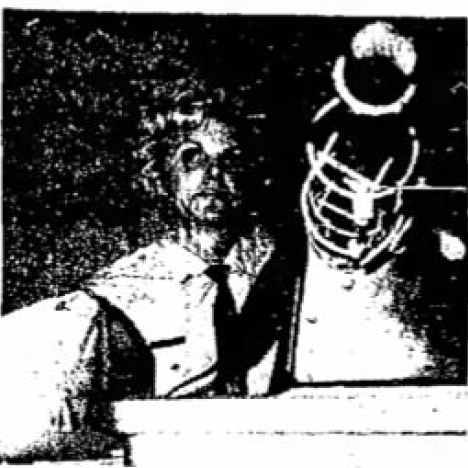
\includegraphics[width=1\linewidth]{img/TheGastoniaGazetteSun1970_10_04} 

}

\caption{Gaston County Sheriff's Deputy Anne Huffsteller poses with a thermal fogger (\protect\hyperlink{ref-TheGastoniaGazetteSun1970_10_04}{The Gastonian Gazette Sun 1970b}).}\label{fig:imgTheGastoniaGazetteSun19701004}
\end{figure}

Apparently the threat of \protect\hyperlink{BigMac}{death by chemical weapons fog} is sufficient to scare detained individuals into compliance.

Within a few years, however, departments began to realize they had no need for the machines, and began selling them with no use aside from testing (\protect\hyperlink{ref-DesMoinesTribune1975_05_06}{Des Moines Tribune 1975}).
The Storm Lake Iowa (1970 pop. 8,591; \protect\hyperlink{ref-USCB1970}{USCB} (\protect\hyperlink{ref-USCB1970}{1971})) purchased a fogger in 1971 in advance of a motorcycle rally that never happened, and used free advertising in local media in attempts to pawn it (\protect\hyperlink{ref-DesMoinesTribune1975_05_06}{Des Moines Tribune 1975}).
The article/ad mentions that officers have used foggers ``on occasion'' in Des Moines (Iowa's capital; 1970 pop. 201,404; \protect\hyperlink{ref-USCB1970}{USCB} (\protect\hyperlink{ref-USCB1970}{1971})) in addition to \protect\hyperlink{IowaCity}{one instance on the University of Iowa's campus} (\protect\hyperlink{ref-DesMoinesTribune1975_05_06}{Des Moines Tribune 1975}), although I have not located contemporaneous mentions.

\hypertarget{Canada}{%
\section{Crossing to Canada}\label{Canada}}

Canadian law enforcement was also quick to jump on the fogger train and the media were just as happy to propagandize their use (\protect\hyperlink{ref-Patterson1976}{Patterson 1976}).
A convention of US and Canadian police chiefs held in Halifax, Nova Scotia in 1976 provided a glimpse into the state of affairs by mid-decade, at which point a supply chain had clearly been developed, although weapons salesmen refused to be named or have their statements linked to employers (\protect\hyperlink{ref-Patterson1976}{Patterson 1976}).



\begin{figure}

{\centering 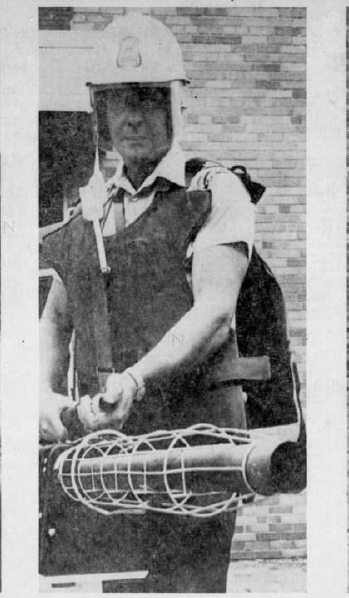
\includegraphics[width=0.75\linewidth]{img/MacKenzie1976} 

}

\caption{Sergeant Al Oakley shows off a pepper fogger (\protect\hyperlink{ref-MacKenzie1976}{MacKenzie 1976}).}\label{fig:imgMacKenzie1976}
\end{figure}

\hypertarget{scholastic-endeavors}{%
\chapter{Scholastic Endeavors}\label{scholastic-endeavors}}

Perhaps instigated by the willingness of the California Highway Patrol to use chemical weapons (including thermal foggers) in \protect\hyperlink{BerkeleyCA1968_08_31}{Berkeley on and around the University of California campus during the 1968 Convention protests}, many law enforcement agencies escalated anti-war and racial just protests in University towns during the 1960s and 1970s via chemical weapons.

The willingness of police to fog literally any place where undergraduates standing up for racial justice and against imperialism were gathering was highlighted in May of 1970 when \protect\hyperlink{CollegeParkMD1970_05_04}{Maryland State Police deployed chemical weapons via thermal fogger into the University of Maryland Chapel} (\protect\hyperlink{ref-Cabe1970}{Cabe 1970}).

Use of fogger-based chemical weapons against students, particularly students of color, was not limited to college campuses, but extended to high and middle schools.

\hypertarget{university-cities}{%
\section{University Cities}\label{university-cities}}

\hypertarget{durham}{%
\subsection{Durham}\label{durham}}

Durham North Carolina Police broke up the ``Allen Building Demonstration'' taking place February 13 1969 on the campus of Duke University in Durham using a variety of weapons, including a thermal fogger (\protect\hyperlink{ref-DMH1969}{Jolley and Olive 1969}, \protect\hyperlink{ref-Schreiberetal1971a}{Schreiber et al. 1971a}, \protect\hyperlink{ref-Schreiberetal1971b}{1971b}).
The police reportedly chased protesters across campus with the fogger, including using it inside Duke Chapel (\protect\hyperlink{ref-Schreiberetal1971a}{Schreiber et al. 1971a}, \protect\hyperlink{ref-Schreiberetal1971b}{1971b}).



\begin{figure}

{\centering 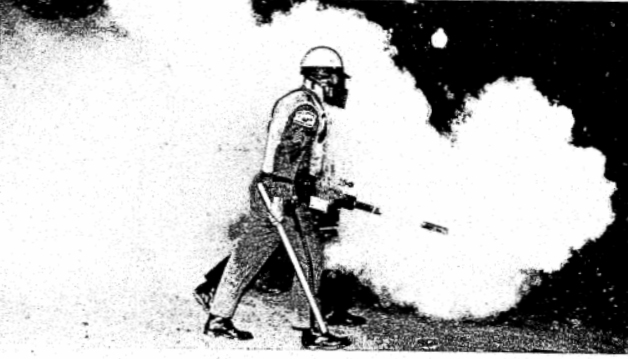
\includegraphics[width=1\linewidth]{img/durham_1969_02_13_1} 

}

\caption{Deployment of a thermal fogger by police on Duke Campus (\protect\hyperlink{ref-DMH1969}{Jolley and Olive 1969}).}\label{fig:imgdurham196902131}
\end{figure}



\begin{figure}

{\centering 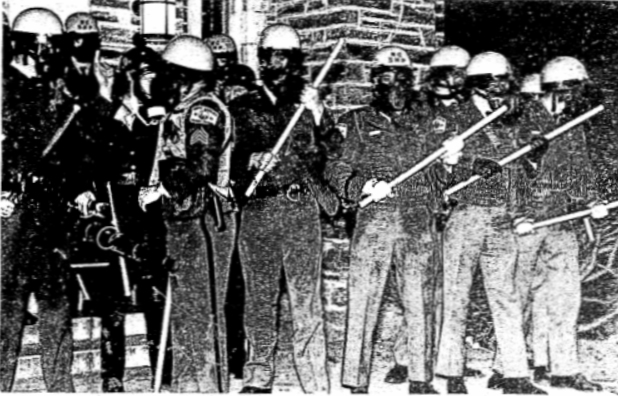
\includegraphics[width=1\linewidth]{img/durham_1969_02_13_2} 

}

\caption{Police with pepper fogger on Duke campus (\protect\hyperlink{ref-DMH1969}{Jolley and Olive 1969}).}\label{fig:imgdurham196902132}
\end{figure}

\hypertarget{berkeley}{%
\subsection{Berkeley}\label{berkeley}}

\hypertarget{BerkeleyCA1969_02_21}{%
\subsubsection{February 21 1969}\label{BerkeleyCA1969_02_21}}

A year after \protect\hyperlink{ChicagoIL1968_08_26}{using the fogger on a protest held in solidarity with the Chicago Protest}, police in Berkeley again deployed a fogger to clear demonstrators including striking students from outside a University Regents and Sproul Hall plaza on the University of California campus.



\begin{figure}

{\centering 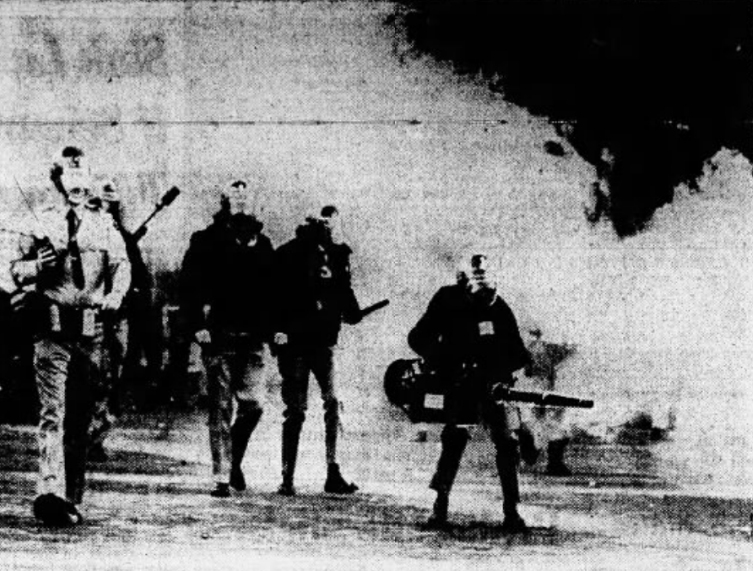
\includegraphics[width=1\linewidth]{img/berkeley_1969_02_21a} 

}

\caption{Police use a pepper fogger and other chemical weapons to clear a University plaza (\protect\hyperlink{ref-APphoto1969a}{Associated Press 1969j}).}\label{fig:imgberkeley19690221a}
\end{figure}

This deployment was covered in papers across the country including the Press-Telegram (Long Beach, California) (\protect\hyperlink{ref-PressTelegram1969_02_21}{Associated Press 1969b}), The Jackson Sun (Jackson, Tennessee) (\protect\hyperlink{ref-TheJacksonSun1969_02_21}{Associated Press 1969c}), The Daily Tribune (Wisconsin Rapids, Wisconsin) (\protect\hyperlink{ref-TheDailyTribune1969_02_21}{Associated Press 1969a}), The Sumter Daily Item (Sumter, South Carolina) (\protect\hyperlink{ref-TheSumterDailyItem1969_02_21}{Associated Press 1969d}), The New Mexican (Santa Fe, New Mexico) (\protect\hyperlink{ref-TheNewMexican1969_02_21}{Associated Press 1969e}), Janesville Daily Gazette (Janesville, Wisconsin) (\protect\hyperlink{ref-JanesvilleDailyGazette1969_02_22}{Associated Press 1969h}), and Messenger-Inquirer (Owensboro, Kentucky) (\protect\hyperlink{ref-MessengerInquirer1969_02_22}{Associated Press 1969i}).



\begin{figure}

{\centering 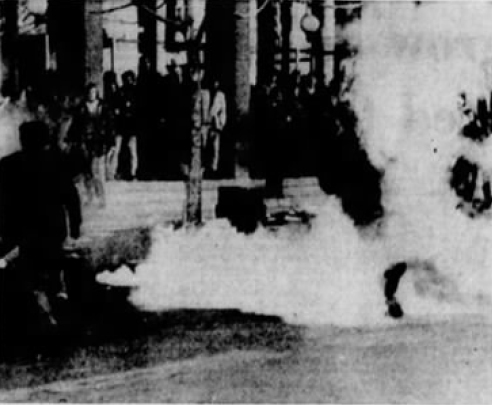
\includegraphics[width=1\linewidth]{img/berkeley_1969_02_21b} 

}

\caption{Police engulf a University plaza in chemical fog (\protect\hyperlink{ref-APphoto1969a}{Associated Press 1969j}).}\label{fig:imgberkeley19690221b}
\end{figure}

Canadian newspapers detailed the fogger use as well, specifically the Red Deer Advocate Red Deer, Alberta, Canada) (\protect\hyperlink{ref-RedDeerAdvocate1969_02_21}{Associated Press 1969f}) and The Leader-Post (Regina, Saskatchewan) (\protect\hyperlink{ref-TheLeaderPost1969_02_21}{Associated Press 1969g}).

\hypertarget{february-28-1969}{%
\subsubsection{February 28 1969}\label{february-28-1969}}

The following week, the police in Berkeley were joined by California National Guard troops to attack strikers, and continued to use the pepper fogger (\protect\hyperlink{ref-TheMiamiNews1969_03_01}{Associated Press 1969m}, \protect\hyperlink{ref-PressandSunBulletin1969_03_01}{1969n}).



\begin{figure}

{\centering 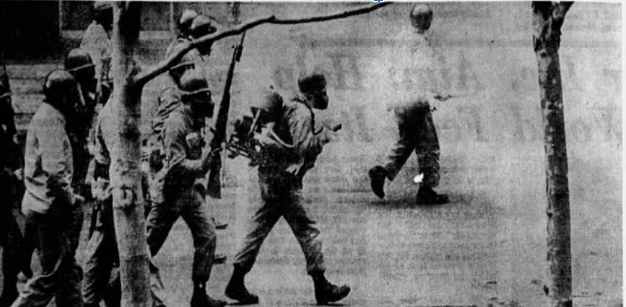
\includegraphics[width=1\linewidth]{img/berkeley_1969_02_28_1} 

}

\caption{National guardsmen and police fog UC Berkeley (\protect\hyperlink{ref-APphoto1969c}{Associated Press 1969k}).}\label{fig:imgberkeley196902281}
\end{figure}



\begin{figure}

{\centering 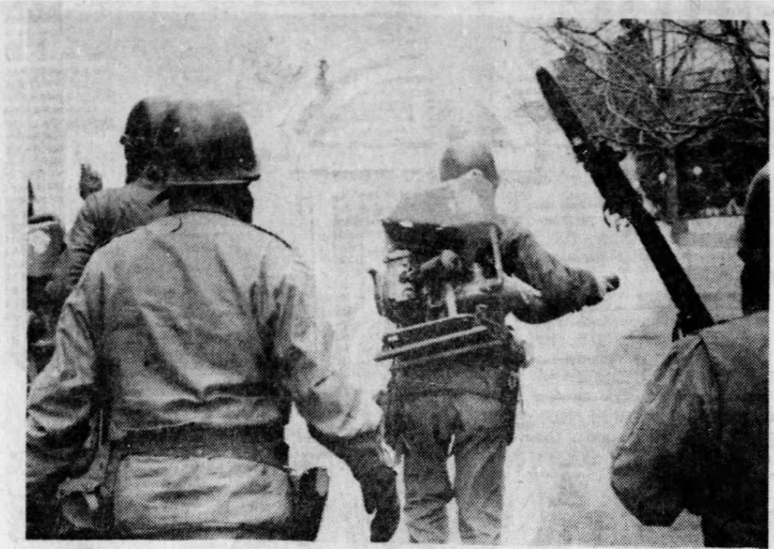
\includegraphics[width=1\linewidth]{img/berkeley_1969_02_28_2} 

}

\caption{View from behind of the police using a pepper fogger on striking students (\protect\hyperlink{ref-APphoto1969d}{Associated Press 1969l}).}\label{fig:imgberkeley196902282}
\end{figure}

\hypertarget{may-15-1969}{%
\subsubsection{May 15 1969}\label{may-15-1969}}

Alameda County sheriffs deployed a pepper fogger on UC Berkeley's campus again during the ``People's Park Riots'' of 1969 (\protect\hyperlink{ref-LATimes1969}{Los Angeles Times 1969}, \protect\hyperlink{ref-Hayes1970}{Hayes 1970}).

The riot apparently started when the university tried to prevent individuals living on the street from a volunteer-run park they built on a lot owned by the school (\protect\hyperlink{ref-ThePressDemocrat1970_10_13}{United Press International 1970}).

The Sheriffs were joined by the California National Guard once again, who this time fogged neighborhoods from the back of a Jeep:



\begin{figure}

{\centering 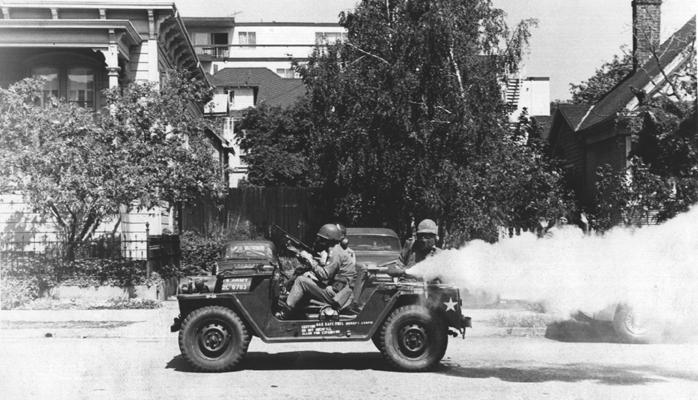
\includegraphics{img/gasjeep} 

}

\caption{California National Guard's Gas Jeep (\protect\hyperlink{ref-gasjeep}{Rosenberg 1969}).}\label{fig:gasjeep}
\end{figure}

\hypertarget{seattle}{%
\subsection{Seattle}\label{seattle}}

Seattle Washington police deployed CN and CS gas via a new pepper fogger in their clash with ``hundreds of unruly youths in the University District'' on August 14 1969 (\protect\hyperlink{ref-StatesmanJournal1969_08_17}{Associated Press 1969p}).
Witnesses recounted that the machine was ``highly effective,'' filling ``2-3 blocks of a street with tear gas in about a minute'' (\protect\hyperlink{ref-StatesmanJournal1969_08_17}{Associated Press 1969p}).

\hypertarget{CollegeParkMD1970_05_04}{%
\subsection{College Park}\label{CollegeParkMD1970_05_04}}

On May 4th 1970, students gathered at campuses around the country to protest President Nixon's expansion of war into Cambodia, inlcuding in at the University of MAryland (UMD) campus in College Park (\protect\hyperlink{ref-WAS2013}{Washington Area Spark 2013}).
Police responded with chemical weapons that did not deter the protest, but rather moved it around the campus (\protect\hyperlink{ref-Cabe1970}{Cabe 1970}).
By later in the day, UMD students had heard about the Ohio National Guard shooting four Kent State students and took up a position in front on and inside the UMD Chapel (\protect\hyperlink{ref-WAS2013}{Washington Area Spark 2013}), which did not stop the chemical weapons barrage or the use of the fogger specifically (\protect\hyperlink{ref-Oates1970}{Oates 1970})



\begin{figure}

{\centering 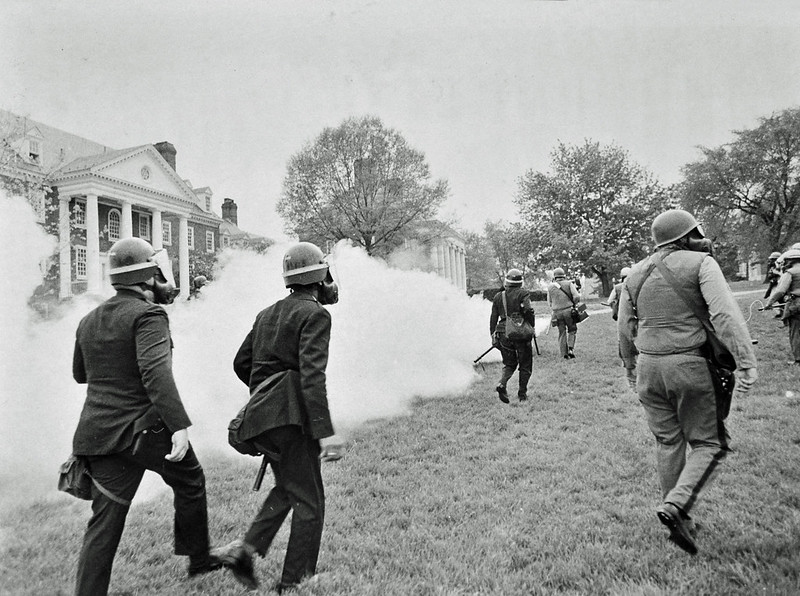
\includegraphics[width=1\linewidth]{img/Cabe1970} 

}

\caption{Police fog the University of Maryland (\protect\hyperlink{ref-Cabe1970}{Cabe 1970}).}\label{fig:imgCabe1970}
\end{figure}



\begin{figure}

{\centering \includegraphics[width=1\linewidth]{img/Oates1970} 

}

\caption{Police fog the University of Maryland Chapel (\protect\hyperlink{ref-Cabe1970}{Cabe 1970}).}\label{fig:imgOates1970}
\end{figure}

The Maryland State Police liked the \protect\hyperlink{GOEC}{GOEC} fogger so much they included it in their Manual on Civil Disturbances as a tool for deploying \href{https://en.wikipedia.org/wiki/CS_gas}{CS gas} (\protect\hyperlink{ref-MSP}{Maryland State Police 1972}):



\begin{figure}

{\centering 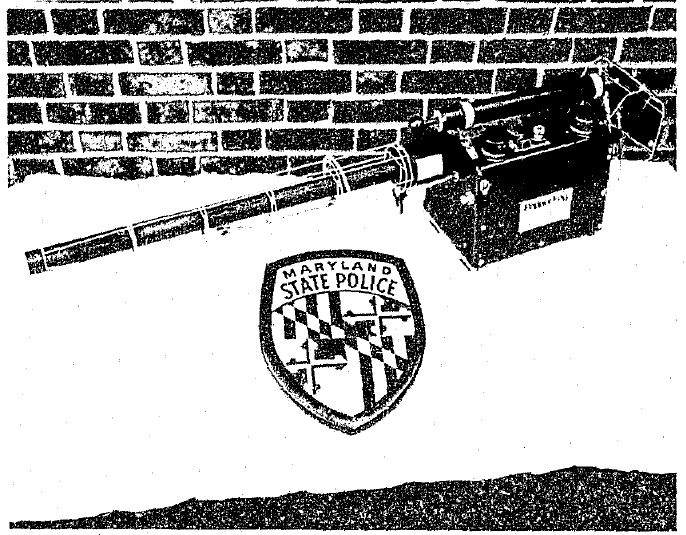
\includegraphics[width=1\linewidth]{img/MSP} 

}

\caption{Maryland State Police's \protect\hyperlink{GOEC}{GOEC} pepper fogger (\protect\hyperlink{ref-MSP}{Maryland State Police 1972}).}\label{fig:imgMSP}
\end{figure}

\hypertarget{IowaCity}{%
\subsection{Iowa City}\label{IowaCity}}

Johnson County sheriffs - including two deputies carrying pepper foggers - used chemical weapons against protesters in Iowa City, Iowa IA on May 6 1971 (\protect\hyperlink{ref-Eckholt1971}{Eckholt 1971}).

The chemicals deployed smelled like insecticides and were described in print as ``unidentified'' because the Sheriff refused to publicly name the compounds, including to the news media (\protect\hyperlink{ref-Eckholt1971}{Eckholt 1971}).

\hypertarget{Minneapolis1972_05_10}{%
\subsection{Minneapolis}\label{Minneapolis1972_05_10}}

Thousands of anti-war protesters gathered in cities around the US on May 10 1972 to demonstrate against the use of mines in Vietnam harbors (\protect\hyperlink{ref-ArgusLeader1972_05_11a}{Associated Press 1972a}).
In Minneapolis, crowds totalling a thousand protestered gathered on and near the University of Minnesota campus and police responded with chemical weapons deployed via grenades, sprays, a helicopter and a thermal fogger (\protect\hyperlink{ref-ArgusLeader1972_05_11b}{Associated Press 1972b}, \protect\hyperlink{ref-StarTribune1972_05_11}{Star Tribune 1972}).

The fogger was used to direct the crowd around campus and spread gas over large areas, such as the area known as Scholars Walk (\textasciitilde0.25 mile from Washington Avenue to the Auditorium) (\protect\hyperlink{ref-StarTribune1972_05_11}{Star Tribune 1972}).

\hypertarget{gainesville}{%
\subsection{Gainesville}\label{gainesville}}

Similarly to the anti-mine protests in \protect\hyperlink{Minneapolis1972_05_10}{Minneapolis}, on the campus of the University of Florida in Gainesville, Florida Highway Patrol deployed a riot vehicle dubbed ``The Monster'' which ``spewed tear gas'' (\protect\hyperlink{ref-ArgusLeader1972_05_11b}{Associated Press 1972b}).
Although a fogger is not mentioned specifically, this is the same agency (Florida Highway Patrol) that first \href{Liberty\%20City\%20\#MiamiFL1968_08_08}{deployed thermal foggers via a truck} in 1968 (\protect\hyperlink{ref-Tschenschlok1995}{Tschenschlok 1995}, \protect\hyperlink{ref-Lorentzen2018}{Lorentze 2018}).

\hypertarget{high-schools}{%
\section{High Schools}\label{high-schools}}

As soon as they laid their hands on foggers, law enforcement extended their use from \protect\hypertarget{Universities}{}{universities} to high schools, specifically using the weapons against Black youth protesters.

I will stop to repeat that again so that we (myself included) can all reflect on this.

Law enforcement agents used chemical weapons against Black junior and high school students during the Civil Rights Era, including a weapon (the thermal fogger) developed not even five years prior to \protect\hyperlink{Vietnam}{gas Vietnamese soldiers and civilians from tunnels}.

\hypertarget{SanGordonio}{%
\subsection{San Gordonio}\label{SanGordonio}}

Although undated, this photograph printed in The Delta Democrat-Times (Greenville, Mississippi Thursday) (\protect\hyperlink{ref-TheDeltaDemocratTimes1969_11_20}{United Press International 1969a}) on November 20, 1969 references a ``recent'' use of the fogger on students.



\begin{figure}

{\centering 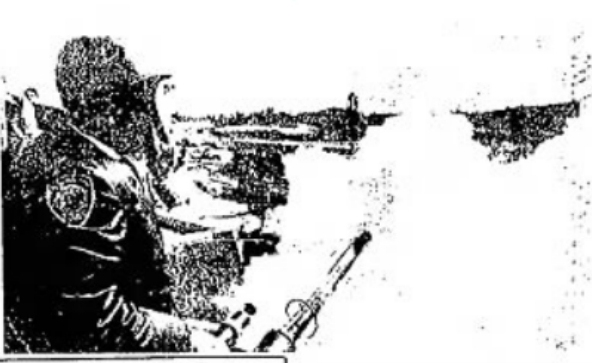
\includegraphics[width=1\linewidth]{img/san_bernardino_1969_xx_xx} 

}

\caption{Police use a pepper fogger on students at San Gordonio High School (\protect\hyperlink{ref-UPIphoto1969}{United Press International 1969b}).}\label{fig:imgsanbernardino1969xxxx}
\end{figure}

Use of the thermal fogger by police that day seems likely, given their more documented deployment of it on December 3, 1971.
On that day, a combination of San Bernardino police, San Bernardino County sheriffs, and California Highway Patrol used tear gas from a pepper fogger to break up a ``major racial confrontation'' among students at San Gorgonio High School and across a 20-block area surrounding campus (\protect\hyperlink{ref-Yetzeretal1971}{Yetzer et al. 1971}).

\hypertarget{Lawrence1970_04_21}{%
\subsection{Lawrence}\label{Lawrence1970_04_21}}

Lawrence, Kansas Police used tear gas, including from a thermal fogger, on April 21st, 1970 against Black high school and junior high students, their parents, and community members (\protect\hyperlink{ref-Monhollon2002}{Monhollon 2002}).
The students had gathered that day after a week-long stand-off with administration in response to their failures to meet their demands regarding Black representation in curriculum, hiring, sports, and awards (\protect\hyperlink{ref-Monhollon2002}{Monhollon 2002}).

Black students had occuppied the principal's office on May 13th and prominent members of the office occupation were arrested from the school that day and promptly suspended from school (\protect\hyperlink{ref-Monhollon2002}{Monhollon 2002}).
Racial tensions escalated over the subsequent week flamed by presence and actions of the local Klu Klux Klan and Minutemen, some of whom were also police officers (\protect\hyperlink{ref-Monhollon2002}{Monhollon 2002}).
The night of April 20th, the school board held a meeting where they barred suspended students from participating and did not reinstate them, nor did they address the demands, and there was a mass walkout (\protect\hyperlink{ref-Monhollon2002}{Monhollon 2002}).

The next day, police were ready with heavy chemical weaponry, including the \protect\hyperlink{GOEC}{GOEC Pepper Fog} fogger:



\begin{figure}

{\centering 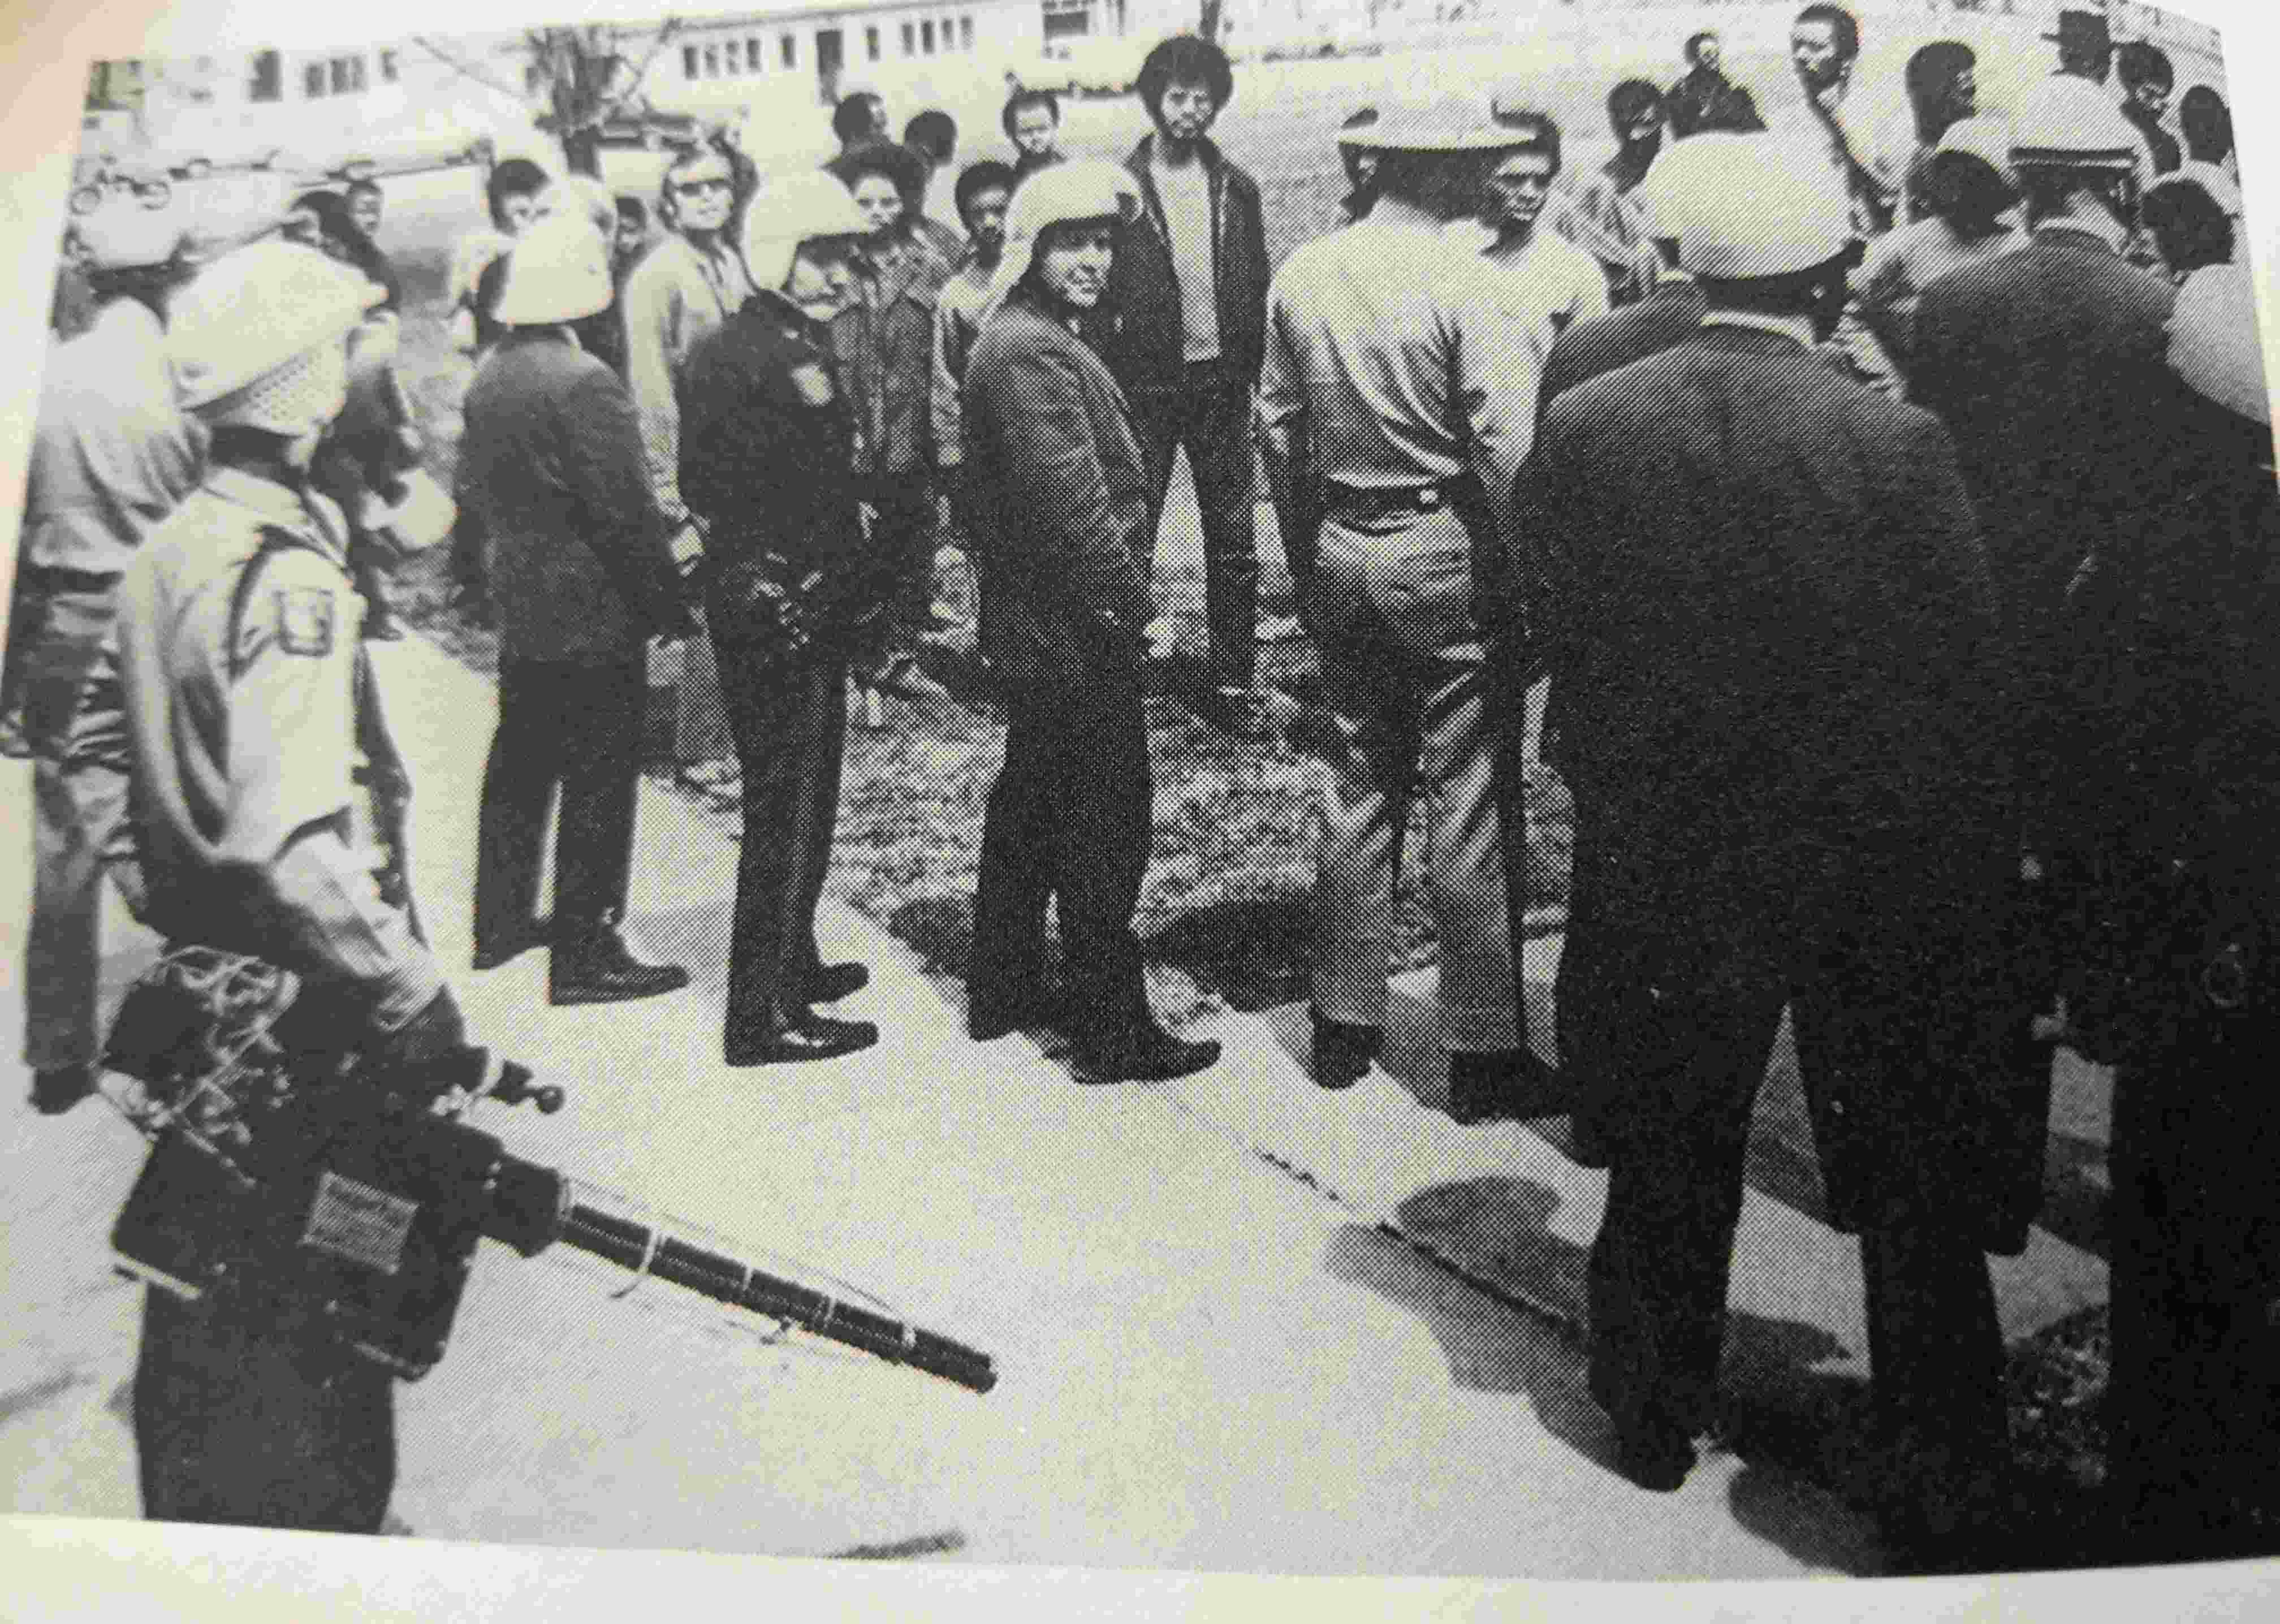
\includegraphics[width=1\linewidth]{img/lawrence_1970_04_21} 

}

\caption{Police bring a \protect\hyperlink{GOEC}{GOEC} pepper fogger to gas Black high school and junior high students at Lawrence High School (\protect\hyperlink{ref-UKA1970}{University of Kansas Archives 1970}).}\label{fig:imglawrence19700421}
\end{figure}

\hypertarget{broadening-application}{%
\chapter{Broadening Application}\label{broadening-application}}

The use of foggers, while not commonly overt, spread throughout the 1970s and 1980s, occasionally making an appearance in news media reports.

\hypertarget{racial-justice}{%
\section{Racial Justice}\label{racial-justice}}

Police are generally more apt to use heavy responses including chemical weapons against Black protesters in general (\protect\hyperlink{ref-DSPDX2020}{Morman et al. 2020}).
It is therefore not surprising to learn that law enforcement use foggers to deploy chemical weapons on racial justice protests.
Indeed, the first use of the fogger in the United States was during the \protect\hyperlink{MiamiFL1968_08_08}{Liberty City Riots}, a police action in response to Black community organizations holding conversation among themselves.

\hypertarget{danville-illinois}{%
\subsection{Danville, Illinois}\label{danville-illinois}}

Foggers have been used in a variety of cities, not just major metropolitan areas.

Danville, Illinois (1970 pop. 42,570; (\protect\hyperlink{ref-USCB1970}{USCB 1971})) Police used a pepper fogger to disperse a crowd of Black protesters that had used picnic tables to barricade a street through their neighborhood on a second night of demonstrations (\protect\hyperlink{ref-Palladium-Item1969}{Associated Press 1969o}), August 10th 1969.

\hypertarget{rodney-king}{%
\subsection{Rodney King}\label{rodney-king}}

Although mentioned in a few outlets during the 1992 police response to the protests in response to the verdict in the Rodney King case, I have yet to find documentation of foggers being used explicitly during that time (\protect\hyperlink{ref-Askren1992}{Askren 1992}).
For example, Riley County (Kansas; 1970 pop. 56,788; \protect\hyperlink{ref-USCB1970}{USCB} (\protect\hyperlink{ref-USCB1970}{1971})) Sheriffs had a fogger in their arsenal in 1992 according to Director Alvan Johnson (\protect\hyperlink{ref-Askren1992}{Askren 1992}).

\hypertarget{labor}{%
\section{Labor}\label{labor}}

Another common target of police force are labor activists, and so it is not suprising to see the fogger being deployed against strikers at least once in US history.

\hypertarget{north-kingstown-rhode-island}{%
\subsection{North Kingstown, Rhode Island}\label{north-kingstown-rhode-island}}

On March 22 1982, the Brown and Sharpe company called in local police and Rhode Island State Police officers to help try to break a (at the time) 22-long strike at their factory in North Kingstown, Rhode Island (\protect\hyperlink{ref-TheLexingtonHerald1982_03_23}{Associated Press 1982b}, \protect\hyperlink{ref-Carbone2017}{Carbone 2017}).
A North Kingstown officer named TJ Varone deployed tear gas via a pepper fogger on a group of 75 people, primarily workers' wives and Brown University students, that was blocking the main entrance to the tool factory (\protect\hyperlink{ref-TheLexingtonHerald1982_03_23}{Associated Press 1982b}, \protect\hyperlink{ref-Carbone2017}{Carbone 2017}).
The picketers braved the gas for a considerable amount of time, requiring close-range fogging to finally disperse them (\protect\hyperlink{ref-Carbone2017}{Carbone 2017}).



\begin{figure}

{\centering \includegraphics[width=1\linewidth]{img/north_Kingstown_1982_3_22} 

}

\caption{Police fog striking workers and their families (\protect\hyperlink{ref-APphoto1982}{Associated Press 1982a}).}\label{fig:imgnorthKingstown1982322}
\end{figure}

The fogging did not, however, break the strike (\protect\hyperlink{ref-Carbone2017}{Carbone 2017}).

Newspaper and television coverage of the fogging circled the globe (\protect\hyperlink{ref-Carbone2017}{Carbone 2017}).

\hypertarget{celebrations}{%
\section{Celebrations}\label{celebrations}}

On occasion, police forces have used foggers against protests or riots that are more of a celebratory nature but still do not respond to their commands to disperse.

\hypertarget{nhra-nationals}{%
\subsection{1974 NHRA Nationals}\label{nhra-nationals}}

Indiana State Police used a pepper fogger and gas grenades on a crowd of 2,000 drag racing fans blocking a highway between the track and campsites at the Hot Rod Association's US Nationals in Clermont IN, September 1 1974 (\protect\hyperlink{ref-Courier1974_09_02}{Associated Press 1974a}, \protect\hyperlink{ref-TheBillingsGazette1982_01_10}{1974b}).

\hypertarget{new-years-eve}{%
\subsection{1975 New Years Eve}\label{new-years-eve}}

New Year's Eve 1975 was apparently quite raucous in Florida, as many cities experienced revelry that got out-of-hand enough to elicit police use of force (\protect\hyperlink{ref-TheTampaTribune1976_01_02}{United Press International 1976a}).
In Ft. Lauderdale, party-goers pulled down a traffic light and police deployed multiple foggers on a crowd of 2,500 on the beach (\protect\hyperlink{ref-TheTampaTribune1976_01_02}{United Press International 1976a}).



\begin{figure}

{\centering 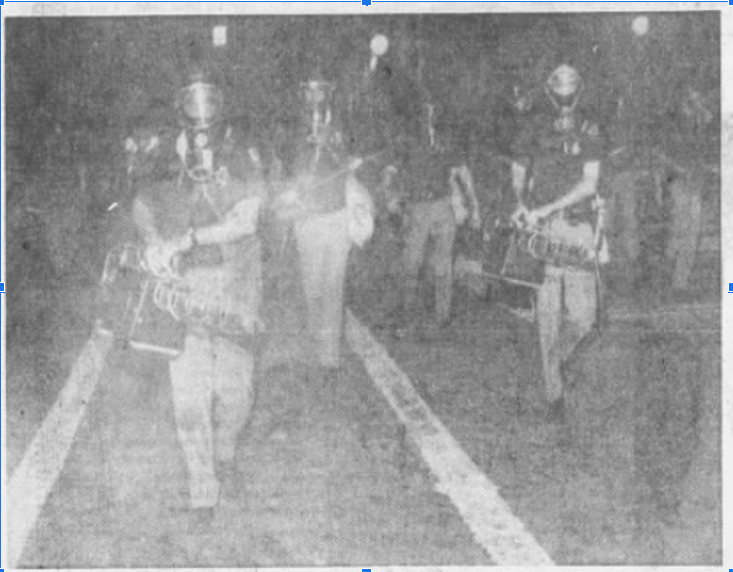
\includegraphics[width=1\linewidth]{img/ft_lauderdale_1975_12_31} 

}

\caption{Police carrying pepper foggers towards the beach (\protect\hyperlink{ref-UPIphoto1975}{United Press International 1975a}).}\label{fig:imgftlauderdale19751231}
\end{figure}

The mayhem was noteworthy enough to garner publication in the Berkeley Gazette (\protect\hyperlink{ref-BerkeleyGazette1976_01_02}{United Press International 1976b}) as well as the Tampa Tribune (\protect\hyperlink{ref-TheTampaTribune1976_01_02}{United Press International 1976a}).

\hypertarget{trainging-accidents}{%
\section{Trainging Accidents}\label{trainging-accidents}}

While not an intentional deployment, in at least one documented incident, a pepper fogger used in firefighter training exercises caused severe symptoms and led to an investigation (\protect\hyperlink{ref-Judd1981}{Judd 1981}).

\hypertarget{bullitt-volunteer-fire-department}{%
\subsection{Bullitt Volunteer Fire Department}\label{bullitt-volunteer-fire-department}}

On December 15 1981, The Southeast Bullitt Volunteer Fire Department In Kentucky was conducting a smoke training exercise using a pepper fogger on loan from the fire marshal's office when their ``victim'' and 16 others (including firefighters) began experiencing coughing fits, headaches, and chest pains (\protect\hyperlink{ref-Judd1981}{Judd 1981}).

Although Smith and Wesson (the Pepper Fogger manufacturer at the time) claimed this was a one-off incident, the Kentucky State Fire Marshal's office had received other reports of firefighters becoming sick when using foggers in smoke training (\protect\hyperlink{ref-Judd1981}{Judd 1981}).
Residue tests later revealed no unexpected compounds (\protect\hyperlink{ref-TheCourierJournal1982_01_10}{The Courier-Journal 1982}), indicating the toxicity had come from the design-for-use ``safe'' smoke.

\hypertarget{CarceralSystem}{%
\chapter{The Carceral System}\label{CarceralSystem}}

Like many chemical weapons devices, thermal foggers are used in local, state, and federal carceral systems.
Unfortunately most deployments go undocumented or such documents never see the light of day.
It seems that the only time we find out about prisoners being fogged is when a serious incident occurs triggering outside investigations and the judicial system.

\hypertarget{BigMac}{%
\section{Big Mac}\label{BigMac}}

In the 1970s, the McAlester (``Big Mac'') Oklahoma State Penitentiary was the site of considerable resistance and rioting by inmates (\protect\hyperlink{ref-WinterSoldier1975}{Winter Soldier 1975}, \protect\hyperlink{ref-TheRag1975}{The Rag 1975}).
A major tool used by the guards in retaliation was tear gas, which they deployed via shot shells, grenades, and pepper foggers (\protect\hyperlink{ref-Allen1974a}{Allen 1974a}, \protect\hyperlink{ref-Allen1975a}{1975a}, \protect\hyperlink{ref-Allen1975b}{1975b}, \protect\hyperlink{ref-Coffey1975b}{Coffey 1975b}).
Given its use here, it is highly likely that the Oklahoma State Penitentiary system used pepper foggers before (and likely after) (\protect\hyperlink{ref-Johnson1974}{Johnson 1974}).

The guards regularly isolated the uprising's leaders in the solitary confinement building known as ``The Rock,'' sealed the building, and gassed it so thick it lasted for days (\protect\hyperlink{ref-Allen1974b}{Allen 1974b}, \protect\hyperlink{ref-TheRag1975}{The Rag 1975}).
During the May 20 1974 gassings in response to riots, Black prisoner Robert Forsythe, a 33-year old serving time for a robbery, happened to be in solitary confinement due to being caught with contraband money and was not associated with the uprising directly, and so inexperienced with the effects of gas (\protect\hyperlink{ref-Johnson1974}{Johnson 1974}, \protect\hyperlink{ref-TheRag1975}{The Rag 1975}, \protect\hyperlink{ref-Wilson1993}{Wilson 1993}).
Although reports are conflicting on details, guards started fogging and gassing prisoners who were, at most, rattling their doors (\protect\hyperlink{ref-Hobbs1974}{Hobbs 1974}).
The likely reason for the barrage was retaliatory, as it was ``unjustified'' according to a veteran guard (\protect\hyperlink{ref-Coffey1975a}{Coffey 1975a}).

During the gassings, a pepper fogger was specifically used in the building and created ``fumes of gas {[}that{]} were awfully heavy, one of the worst I've ever seen'' according to veteran corrections officers' trial testimony (\protect\hyperlink{ref-Allen1975b}{Allen 1975b}, \protect\hyperlink{ref-Coffey1975a}{Coffey 1975a}).
The gassing lasted for four hours despite yells for help, resulting in serious injuries including burned and blistered skin, eyes swollen shut, and breathing difficulties (\protect\hyperlink{ref-Coffey1975b}{Coffey 1975b}).
That intense fogging and lack of medical attention over the next two days were main factors contributing to Forsythe's injuries and death two days later, according to medical experts' testimony (\protect\hyperlink{ref-Allen1974b}{Allen 1974b}, \protect\hyperlink{ref-Allen1975a}{1975a}, \protect\hyperlink{ref-Allen1975b}{1975b}).

Although the guards involved were indicted by a grand jury and brought to trial, they ultimately were acquitted of all charges (\protect\hyperlink{ref-UPI1975a}{United Press International 1975b}, \protect\hyperlink{ref-UPI1975b}{1975c}).

\hypertarget{union-correctional}{%
\section{Union Correctional}\label{union-correctional}}

According to the superintendent, a riot was caused in the Florida State Prison's Union Correctional Institution in Raiford on July 5th, 1981 by 22 prisoners who were intoxicated, and the only way to subdue them was to deploy a thermal fogger (\protect\hyperlink{ref-TallahasseeDemocrat1981_07_07}{United Press International 1981}).
As a result of two officers being ``slightly injured'' and three inmates being stabbed, an investigation was launched that caused the event to be picked up in the newspapers (\protect\hyperlink{ref-TallahasseeDemocrat1981_07_07}{United Press International 1981}).

\hypertarget{dade-county}{%
\section{Dade County}\label{dade-county}}

Dade County Sheriffs used foggers to sweep a field on July 17th 1974 in search of a murder suspect that had eluded K-9 units, helicopters, a plane, and an attempt to flush him out by burning the field (\protect\hyperlink{ref-TampaBayTimes1974_07_18}{Associated Press and United Press International 1974}).
The suspect was so well dug in that he could withstand significant gassing that surprised a Sheriff's sergeant who participated in the operation (\protect\hyperlink{ref-TampaBayTimes1974_07_18}{Associated Press and United Press International 1974}).

\hypertarget{CBP}{%
\chapter{Border Patrol: A Second Boomeranging}\label{CBP}}

United States Border Patrol (BP) has played an outsized role in policing and corrections within the federal immigration system and abroad both in support of armed services and independently (\protect\hyperlink{ref-Miller2019}{Miller 2019}).
Indeed, BP has provided another boomeranging of the Imperial Tetherball that bridges the Vietnam-era and present-day domestic applications via export to foreign governments for use in controling their own populaces.

\hypertarget{international-trafficking}{%
\section{International Trafficking}\label{international-trafficking}}

Within a year and a half of the fogger's arrival to US domestic police agencies, BP agents were engaging foreign governments independent of the military on chemical weapons deployment including using thermal foggers.
During April 25 - May 9 of 1970, Raymond Dee Bond, a Border Patrol agent with decades of experience, sold \$15,000 worth of chemical weaponry to the Mexican federal government (\protect\hyperlink{ref-ValleyMorningStar1973_08_04}{Star Tribune 1973}).
Included in the cache were multiple pepper foggers and formulations (\protect\hyperlink{ref-ValleyMorningStar1973_08_04}{Star Tribune 1973}).
Bond was caught and charges with weapons trafficking and acting as a foreign agent without notifying the Secretary of State (\protect\hyperlink{ref-DailyNews1972_10_27}{United Press International 1972}).
Although indicted by a federal grand jury, Bond was able to escape prosecution by resigning from his position (\protect\hyperlink{ref-ValleyMorningStar1973_08_04}{Star Tribune 1973}).

Given the extensive reach of Border Patrol into Central and South America fueled in particular by the `Drug War' (\protect\hyperlink{ref-Chepesiuk1999}{Chepesiuk 1999}), it is reasonable to expect that this was not an isolated event.

\hypertarget{bortac}{%
\section{BORTAC}\label{bortac}}

By 2020, the Border Patrol Tactical Unit (BORTAC) had been established to, among other tasks, provide particularly extreme responses to domestic as well as foreign uprisings (\protect\hyperlink{ref-CBP2006}{USCBP 2006}, \protect\hyperlink{ref-CBP2014}{2014}, \protect\hyperlink{ref-CBP2018}{2018}).
BORTAC is truly a global domestic law enforcement agency, operating in 28 countries (they were willing to publicly disclose as of 2006; \protect\hyperlink{ref-CBP2006}{USCBP} (\protect\hyperlink{ref-CBP2006}{2006})), providing a wide range of services (\protect\hyperlink{ref-CBP2014}{USCBP 2014}, \protect\hyperlink{ref-Miller2019}{Miller 2019}).
BORTAC's specific genesis was focused on riots in federal immigration detention centers (\protect\hyperlink{ref-CBP2006}{USCBP 2006}, \protect\hyperlink{ref-CBP2014}{2014}), noteworthy given the use of thermal foggers in the United States \protect\hyperlink{CarceralSystem}{carceral system}.

Border Patrol agents from the El Paso unit specifically were deployed to police protests in El Paso in addition to being sent to Portland and other cities like Albuquerque, New Mexico (\protect\hyperlink{ref-Borunda2020}{Borunda 2020}).

\hypertarget{PortlandOR2020_2021}{%
\subsection{Portland OR}\label{PortlandOR2020_2021}}

The thermal fogger made a very visible return to the public sphere in July of 2020, when US Customs and Border Protection (CBP) officers brought a bright-green version to Portland, OR during the \protect\hyperlink{PortlandOR2020_07_29}{2020 Black Lives Matter protests} (\protect\hyperlink{ref-pb20202021}{PB2020 Team 2021}).
Since then, the fogger has been deployed \protect\hyperlink{PortlandORICE2020_2021}{three additional times by CBP in Portland}, all at the property Immigration and Customs Enforcement (ICE) rents on the South Waterfront.

\hypertarget{PortlandOR2020_07_29}{%
\subsubsection{July 29 2020}\label{PortlandOR2020_07_29}}

At the beginning of July 2020, then-president Trump deployed Department of Homeland Security (DHS) agents to ``protect'' federal property in Portland, OR (\protect\hyperlink{ref-Trump2020}{Trump 2020}, \protect\hyperlink{ref-DHS2020}{USDHS 2020}, \protect\hyperlink{ref-Flanigan2020}{Flanigan 2020}).
During the final days of the visible presence and response of federal agents in Summer 2020, Customs and Border Protection (CBP) unveiled their thermal fogger (\protect\hyperlink{ref-Recompiler2020_07_29}{Sal 2020a}), which has been identified through photos as an \href{https://www.nixalite.com/product/igeba-tf-35}{IGEBA TF35} thermal fogger from Nixalite of America Inc.
This machine is designed and marketed for bird control, and while ``\emph{training tool for military/law enforcement}'' is listed among its uses (\protect\hyperlink{ref-Nixalite2009a}{Nixalite 2009b}), its safety requirements explicitly state:

\begin{quote}
``\emph{\textbf{19. Do not fog directly against persons\ldots During operation keep distance of minimum {[}10 ft{]}.}}'' - (\protect\hyperlink{ref-Nixalite2009b}{Nixalite 2009a})
\end{quote}



\begin{figure}

{\centering 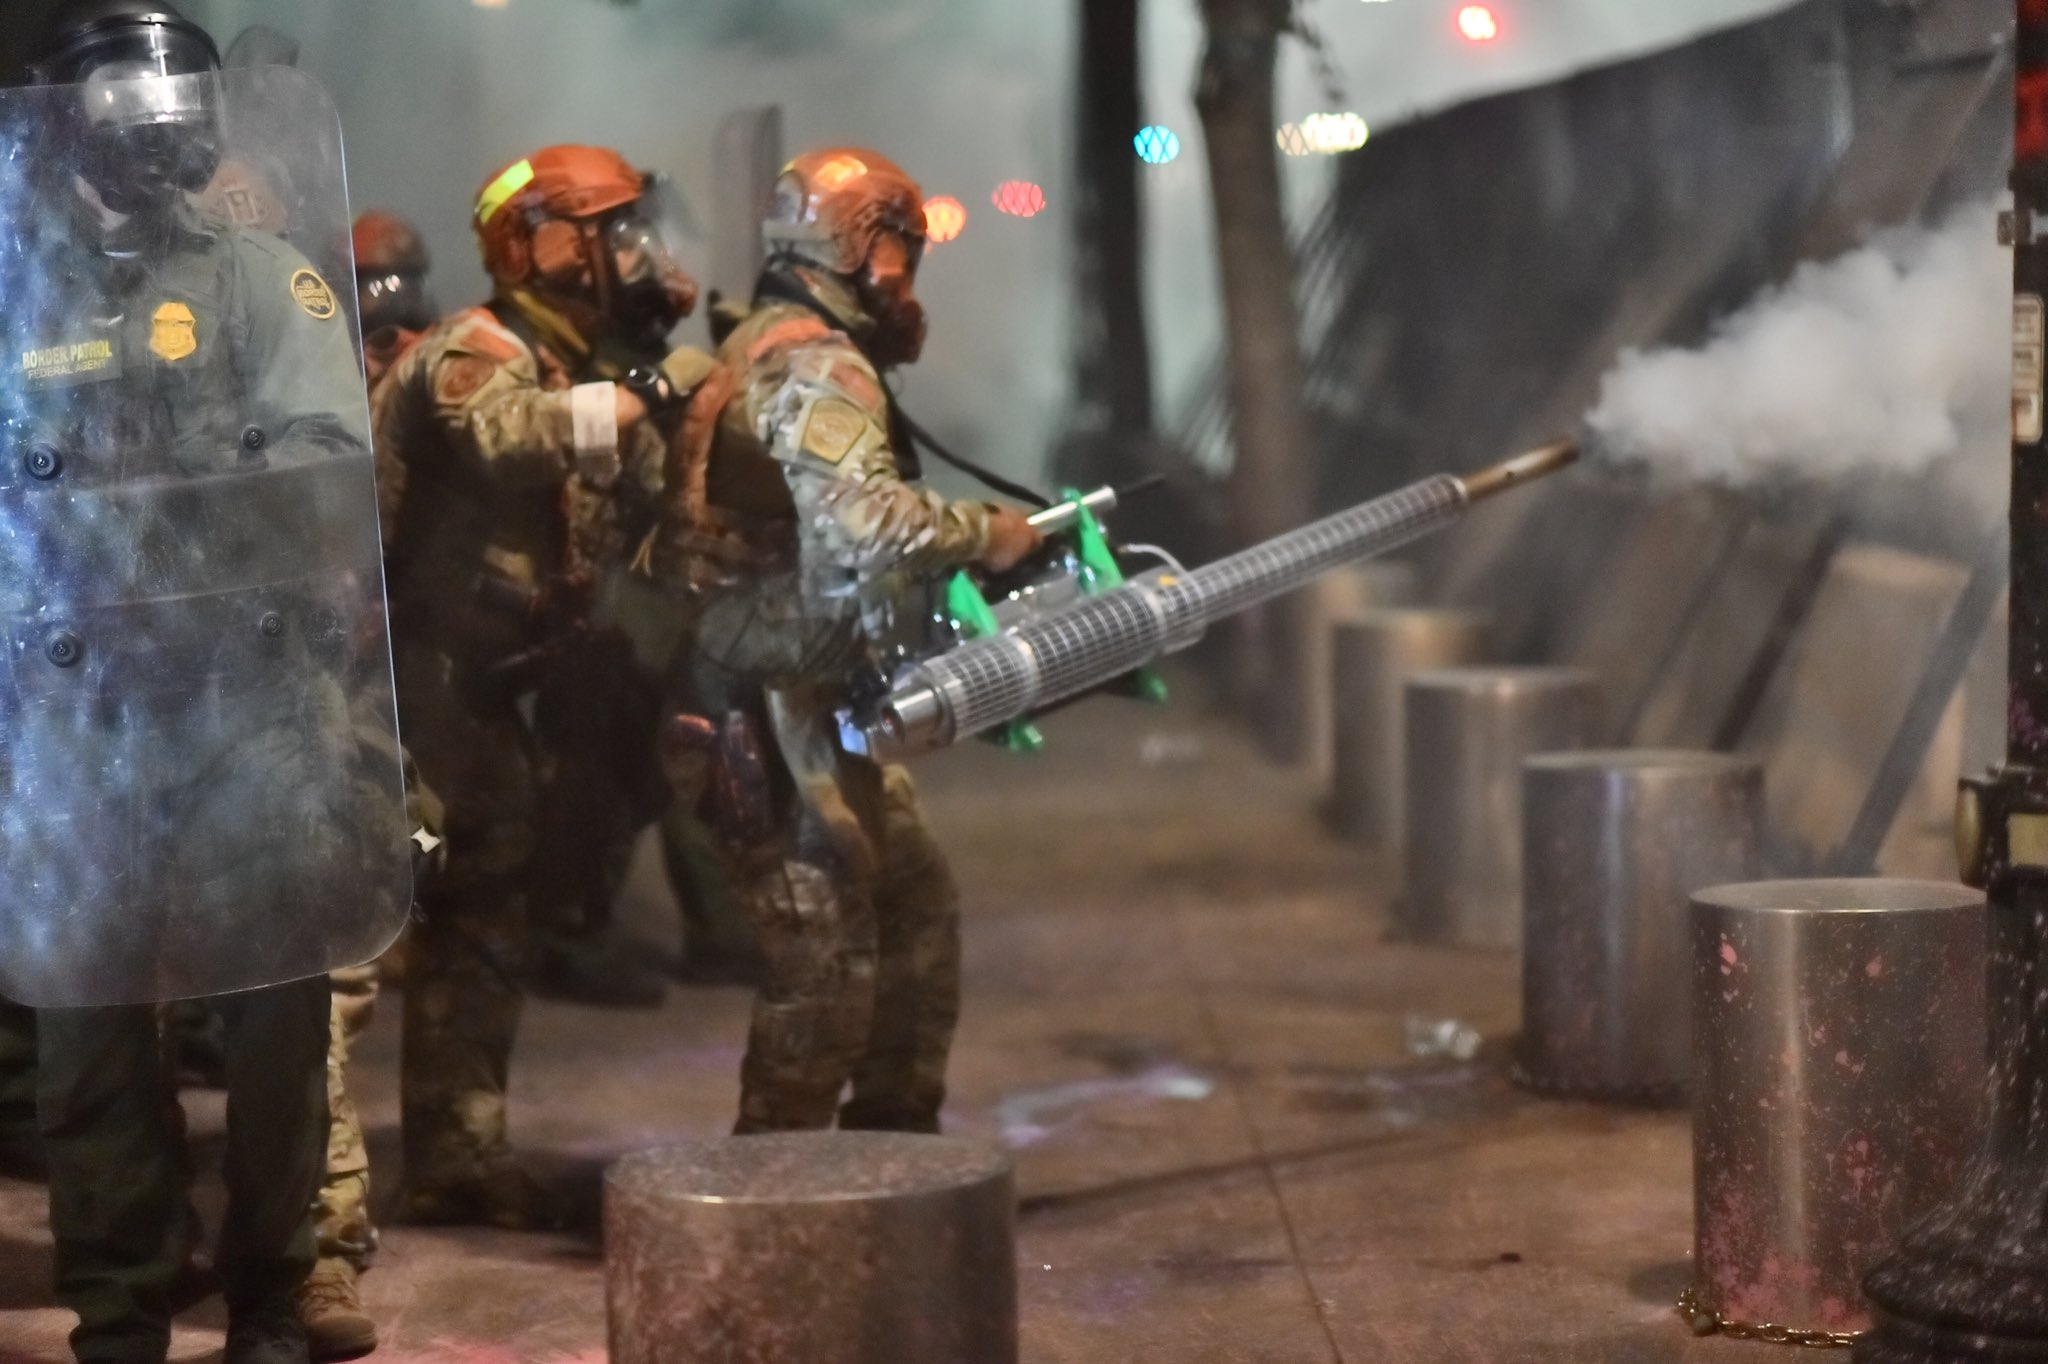
\includegraphics[width=1\linewidth]{img/portland_2020_07_29} 

}

\caption{CBP agent deploying chemical agent via thermal fogger in front of the federal courthouse (\protect\hyperlink{ref-Brown2020}{Brown 2020}).}\label{fig:imgportland202007292}
\end{figure}

\hypertarget{PortlandORICE2020_2021}{%
\subsubsection{Abolish ICE: Immigration and Customs Enforcement Rental Property}\label{PortlandORICE2020_2021}}

While the thermal fogger hasn't been deployed at the federal Courthouse in downtown Portland since July 29 2020, it has been used repeatedly by Department of Homeland Security agents at the private property US Immigration and Customs Enforcement (ICE) rents to use as a holding center for deportees in the South Waterfront neighborhood (\protect\hyperlink{ref-Simonis2021}{Simonis 2021}) -- the same building that saw the weeks-long Ocuppy ICE protests in 2018 (\protect\hyperlink{ref-Dubois2018}{Dubois 2018}).

The first of such deployments occurred during the fall of 2020.

Along with cities across the country, Portland hosted many events on October 17th focused around the racial and gender justice (\protect\hyperlink{ref-Recompiler2020_10_17}{Sal 2020b}).
In the evening, there was a gathering at Willamette Park in the Southwest part of the city, where organizers passed out balloons detailing harrowing experiences of migrants and immigrants detained by ICE (\protect\hyperlink{ref-Recompiler2020_10_17}{Sal 2020b}).
After marching to the ICE rental property, individuals tied the balloons to the gate to the parking garage, and Department of Homeland Security (DHS) agents including Customs and Border Protection (CBP) officers deployed massive amounts of chemical weapons, including via a thermal fogger, throughout the neighborhood (\protect\hyperlink{ref-Recompiler2020_10_17}{Sal 2020b}).



\begin{figure}

{\centering 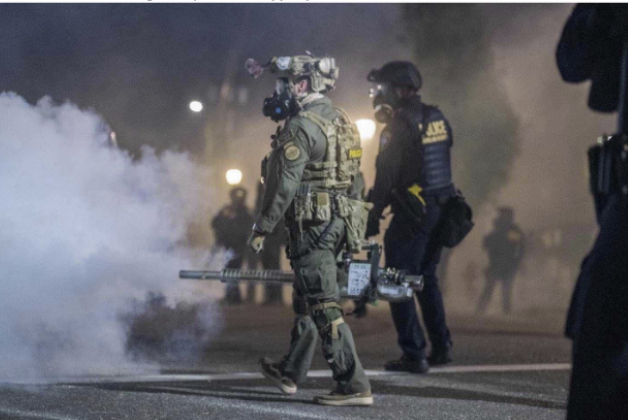
\includegraphics[width=1\linewidth]{img/portland_2020_10_17} 

}

\caption{CBP agent fogging a South Waterfront neighborhood (\protect\hyperlink{ref-Lake2020}{Lake 2020}).}\label{fig:imgportland20201017}
\end{figure}

\hypertarget{J20}{%
\subsubsection{Inaugration 2021}\label{J20}}

The same fogger (or at least the same model) was again brought out at the ICE rental property on January 20th 2021 during the Inauguration Day (``J20'') Abolish ICE protests in response to an individual spray painting a piece of plywood tacked outside the building (\protect\hyperlink{ref-Recompiler2021_01_20}{Sal 2021a}).
The fogged up and down multiple blocks, with visible plumes entering units in the adjacent apartment complexes and covering the playground of an adjacent public school (\protect\hyperlink{ref-Simonis2021}{Simonis 2021}, \protect\hyperlink{ref-Recompiler2021_01_20}{Sal 2021a}).



\begin{figure}

{\centering 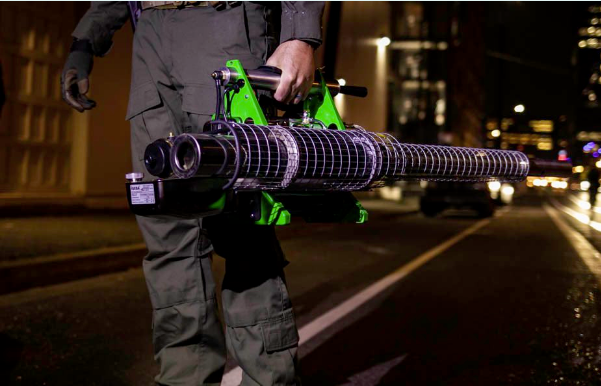
\includegraphics[width=1\linewidth]{img/portland_2021_01_20} 

}

\caption{CBP officer holding thermal fogger (\protect\hyperlink{ref-Staab2021}{Staab 2021}).}\label{fig:imgportland20210120}
\end{figure}

That weekend, CBP deployed the fogger again during Abolish ICE protests, this time gassing even more of the neighborhood, including the local public school and veterans-preference housing (\protect\hyperlink{ref-Simonis2021}{Simonis 2021}, \protect\hyperlink{ref-Recompiler2021_01_23}{Sal 2021b}).



\begin{figure}

{\centering 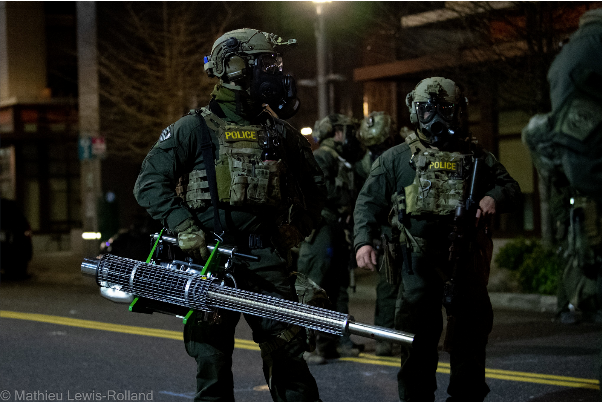
\includegraphics[width=1\linewidth]{img/portland_2021_01_23_1} 

}

\caption{CBP agent holding thermal fogger (\protect\hyperlink{ref-Lewis-Rolland2021a}{Lewis-Rolland 2021a}).}\label{fig:imgportland202101231}
\end{figure}



\begin{figure}

{\centering 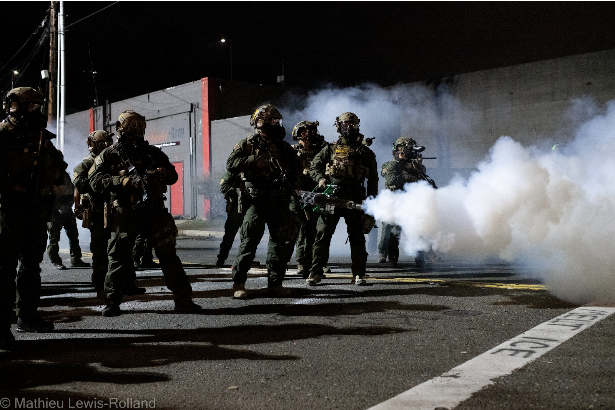
\includegraphics[width=1\linewidth]{img/portland_2021_01_23_2} 

}

\caption{CBP agent fogging an intersection in the South Waterfront neighborhood (\protect\hyperlink{ref-Lewis-Rolland2021b}{Lewis-Rolland 2021b}).}\label{fig:imgportland202101232}
\end{figure}

\hypertarget{Conclusion}{%
\chapter{Conclusion}\label{Conclusion}}

Although the use of a thermal fogger by US CBP to deploy chemical weapons on racial justice protesters in Portland in 2020 and 2021 appeared novel to many, the truth is that it is just the most recent chapter in a cylical narrative stretching back half a century and spanning the globe.

Spawned from the US military occupation of Vietnam, the thermal fogger has always been a tool for suppressing resistance among the populace.
Its initial transition to the American homefront was rapid and smooth, with retired military law enforcement eager to deploy them against civil rights and anti-war protesters.

As the fogger grew less popular with police and faded from public view in the past few decades, its use was maintained in the carceral system
Simultaneously, foggers were peddled by US CBP Agents overseas -- a second deployment.
Agents from the same units within CBP then brought the fogger back home again, for a second return.

Throughout all of this, the fogger was used to maim and even kill individuals while targeting the marginalized, many of whom have stories that have not been heard publicly.
I hope that through this work, I can call attention to the shared history across generations, spark conversations, and facilitate story telling to illuminate the impacts of the thermal fogger on human people beings.

Building on the concept of an Imperial Boomerang, I propose that the trajectory of the thermal fogger can be thought of as an Imperial Tetherball, with multiple departures and returns.
Key questions from my perspective are then:

\begin{itemize}
\tightlist
\item
  what perpetuates the momentum of the fogger, facilitating it to swing around more than once?
\item
  what routes exist for subsequent rotations where the fogger could be deployed overseas and then brought home again?
\end{itemize}

Clearly, this topic deserves more theoretical evaluation, as well.

While the thermal fogger is still presently \emph{in play} in Portland, countless other departments around the world have these machines of war sitting in their arsenals, primed and ready.

And we still don't even know what comes out of the exhaust nozzle.

\cleardoublepage

\hypertarget{appendix-appendices}{%
\appendix \addcontentsline{toc}{chapter}{\appendixname}}


\hypertarget{AltTexts}{%
\chapter{Figure Descriptions}\label{AltTexts}}

Alt-text descriptions for figures in the book:

\begin{itemize}
\item
  Figure \ref{fig:imgportland20200729}: Fully riot-geared and for some reason in green camo US Homeland Security agents (to the middle and the left of the photo) behind a row of two-foot tall, one-foot radius metal posts, behind a metal grate wall over 7 feet tall with metal support beams and concrete pylon buttressing. In the front of the left side is an agent holding a plastic clear riot shield, through which you can see a patch that say `Border Patrol Federal Agent' in yellow and some insignia patches as well. In the middle are the agents in camo, one with a hand on the shoulder of another who is operating a thermal fogger machine shooting gas through the fence. The machine is maybe four or five feet long and has a body not unlike a bush whacker with a two-cycle engine, but fueling a vaporizer instead of a rotor. The agent is holding the machine with their right hand visibly and there is a black strap across their shoulder holding it up. The machine is mostly shiny metal, although the tip is showing signs of corrosion (no surprise based on the compounds and heat) and the supports of the body are a bright green
\item
  Figure \ref{fig:imgCrockett1969}: B/W image drawing with text from an old white paper book. The text says FOG DISSEMINATION at the top then a paragraph with \texttt{Fog\ dissemination\ devices\ operate\ by\ rapidly\ vaporizing\ a\ high\ boiling\ point\ liquid\ agent\ formulation.\ This\ is\ accomplished\ by\ injecting\ the\ liquid\ agent\ into\ a\ hot\ gas\ flow\ and\ allowing\ the\ vaporized\ agent\ to\ contact\ the\ cooler\ ambient\ air\ where\ the\ agent\ condenses\ into\ a\ fog\ and\ ultimately\ into\ extremely\ small\ agent\ particles.} In the middle is the drawing with a square on the left with a long rectangle coming out of it to the right with a cloud out the further end of the rectangle. There are bits of text around it, pointing to the box it says \texttt{FUEL}, \texttt{SPARK}, and \texttt{COMBUSTION\ CHAMBER}. in the middle of the rectange it says \texttt{HOT\ GASES} in the middle of arrows pointing out towards the cloud. Along the rectangle another injection area is noted for \texttt{Liquid\ Agent\ Injection} Text on the bottom says \texttt{FIGURE\ 4.\ FOG\ DISSEMINATION.\ A\ liquid\ chemical\ agent\ is\ vaporized\ by\ a\ hot\ gas\ flow\ and\ released\ as\ a\ fog\ cloud}.
\item
  Figure \ref{fig:imgvcmm}: Book illustration (colorful, hand-rendered style) of green-clad US military service members in helmets flak vests, boots, etc, standing around a thermal fogger in the foreground. The fogger is a non-portable Mity Mite style fogger with a big reservoir and giant vacuum style hose running through a green tarp that's lying on the ground and covering the tunnel entrance. They are in a clearing with huts and the jungle in the background.
\item
  Figure \ref{fig:imgtunnels}: Book illustration (blank and greys, hand-rendered style) of a two-level village tunnel system, connecting most of the structures with defensive trenches and bunkers. There are eight houses surrounding a community building and the nearest ones are cut-away so you can see into them and the ground beneath them, which shows the tunnels and bunkers. Each house has a shelter and they are connected via tunnels. There is a puji-stake moat with a sharpened bamboo fence around it surrounding the village and there's one road in, with a gate at the fence. There is a river or open water of some kind on the other side of the fence and then some fields and jungle. The community building is two stories and is next to a single flag on a pole in the center of the village. The flag is blank, and so functionally white.
\item
  Figure \ref{fig:imgratmask}: B/W image. Open trench at bottom, center. Pipe runs across trench and into the dirt on either side. Person in gas mask crouched below pipe looking up and forward. Leg in pants and lace up boot stretched over trench leaning against right edge. Other leg and boot partially visible on left. Hand holding lit cigarette resting on foot on left.
\item
  Figure \ref{fig:imgirontriangle}: Text-book style map of the III Corps Tactical Zone from 1965-1967, according to the legend. This is the area of Vietnam around Saigon, with some of the South China Sea visible to the south at the bottom and Cambodia to the north west in the upper left portion. Major highways and cities are indicated on the map, but the main points are the color highlighted boundaries of the two war zones and the iron triangle, which are all in reddish organge, and the full tactical zone in a darker blue. There is text in the bottom left that says Map 13 and there is a unit bar in the legend that gives distances in both miles and kilometers.
\item
  Figure \ref{fig:imgmitymite}: Technical rendering sketch of a tank with the words Mity Mite on the side. Funnel on bottom of tank leads to exhaust hose below and pipe on bottom of tank has small flexible hose attaching to exhaust hose as well. Exhaust hose comes from below and curves upward to the right. Below the tanks and attached by a frame is a small motor.
\item
  Figure \ref{fig:imgmightymite}: B/W image in a dirt field. Helmeted soldier on one knee with tank strapped on back. Lifting a board with left hand and holding an exhaust tube from the tank under the board with right hand.
\item
  Figure \ref{fig:imgunpacktest}: B/W image. In a clearing in a densely vegetated area, a small tank with an exhaust pipe blowing fog to the right. The cloud of fog covers much of the right side. Towards the back, 2 people wearing helmets and fatigues with sleeves rolled up stand with hands on hips on either side of the fogger, watching it.
\item
  Figure \ref{fig:imgtablea212}: Screen cap of a photo copy of an old report, it's black and white and in bad shape, but legible for the most part. It's Table A.2.1.2, Chemical Sprays and Foggers. There are columns: Device/Model, Manufacturer, Description, Estimated Cost (for development or for purchase), and Status (available already or needing development). There are 6 rows, one for each Device/Model: MK17 Pepper Fog CS-Tear Smoke Generator, MK XII, Turb A Fog Tear Gas Dispenser, Federal Dust Projector 271, Dynafog 70, and a propsed vehicle based fogger based on the mosquito fogging approach.
\item
  Figure \ref{fig:vietnamaus1}: Black and white photo of a Mighty Mite blower on the left and two containers of acetylene in the middle, both containers are metal boxes with labeling in small white text and then some bladder bag on top. There are large vaccum size hozes coming off the blower and going off frame to the right. The scene is the ground of a jungle that has been cleared a little, there are trees and foliage in the background and dense but matted down grass in the fore.
\item
  Figure \ref{fig:imgvietnamaus2}: An individual crouches on the ground next to a blower, facing off to the right, with his left hand slightly resting on it. The photo is aimed down at this person, so the two people looking at the fogger while standing are partially visible from the feet upwards. The photo is an old black and white image and there are items around the sides that are difficult to make out, including potentially a cache of chemical weapons grenades on the right side and some sandbacks in the back.
\item
  Figure \ref{fig:imgM106}: Yellowed black and white photo of a stationary Mighty Mite thermal fogger. It's a backpack fogger, so there's a giant hose that's like a vacuum hose wrapped around in the middle and then another one coming off of the actual backpack, which is upright in the middle back right. there is a metal frame and a large reservoir tank sitting on top of the engine and other aspects of the machinery. There is a tube running out to the end of the hose nose from the back pack. On the right side of the image is a scale bar that makes it seem like the backpack is 24 inches tall.
\item
  Figure \ref{fig:imgjetfogger}: Black and white technical drawing of a hand-held 2-cycle thermal fogger. The drawing is pretty minimal, but shows enough detail, in particular around the engine and fan, to get a sense of how it operates. There are also a few labels pointing out via arrows what the Recould Rope Starter, Fuel Tank, Carrying Handle, Creifugal Blower Assemble, and Air/Agent Exit Ports are, and to the where the Vaporized Agent is injected into the air stream.
\item
  Figure \ref{fig:img298}: Black and white photo of a thermal fogger that is basically a 2-cycle weed-wacker engine on top of a chemical agent metal drum with a nozzle sticking out to the right that is about a yard long, it's dark and has some hardware on it. The drum says Federal Fogger and then other things that are illegible. The drum is a dark color and the main engine is light, with a dark handle and strap.
\item
  Figure \ref{fig:fedlabimg}: Black and white photo of police officer in a gas mask and riot helmet with the shield flipped up and full uniform, but not riot gear. The officer is holding a hand-held fogger that has a white top on the part, some shiny metal in the middle and then dark on the bottom with a dark nozzle that is spewing some fog. The officer is standing in a field in front of a forest.
\item
  Figure \ref{fig:goecpf}: Yellowed black and white photo of a stationary pepper fog thermal fogger pointed to the left sitting by itself. The main body is a square box that's dark with a tag in the middle that's lighter and has dark writing on it that says pepper fog g o e c.~The nozzle points to the left and is a longer thinner tube about twice as long as the main body. It is also dark and has a metal cage around it that is sparse and shiny. There's also a handle and some knobs on the top of the item and something that's a little bit difficult to make out off the back of the main body.
\item
  Figure \ref{fig:imggoecad1969}: Photocopied, blurried black and white magazine spread advertisement for General Ordnance Equipment Company (GOEC). The ad shows both their chemical mace and their fogger, although the fogger takes up 3/4 of the page. The left side has two main panels, one for each weapon, the top is a mace one showing an officer spraying mace into someone's face and the bottom part is the picture of the person fogging the railroad. The right side is an explainer on the pepper fogger that has three photos (including a repeat of the railroad one) at the top, the item image in the middle, and then a whole bunch of specs that are too blury to read
\item
  Figure \ref{fig:imgdefensetechgepf}: Yellow-gold box shape tool with a handle on top, an image of an eagle in flight on the side, and some gauges on top.The back of the box tapers and appears to have switches and controls. Coming out of the front is a long tube that narrows at the end. The tube has a wire cage surrounding it.
\item
  Figure \ref{fig:imgdemo}: Black and white photo of a person using a pepper fogger across some railroad tracks. The person is standing in the mid ground on the left side of the photo and fogging towards the right mid-ground where the train tracks come from. The fog obscures the origins of the tracks off to the background on the right side of the photo. Behind the person on the left side is a taller tree along short building a car and some foliage. Further behind is a ridge of some kind with trees on it. The train tracks are old and partially overgrown.
\item
  Figure \ref{fig:imgVance1970}: Black and white newspaper clipping of an officer standing in front of a open garage door, next to a police car that is partially in frame on the left and front areas. A GOEC-style thermal fogger sits on the hood of the car in front of the officer, pointing towards and to the left of the camera. The officer is wearing beat clothing and a cop hat and also has a shotgun.
\item
  Figure \ref{fig:imgAmanphoto1970}: Black and white newspaper clipping of an officer standing in a field just front a forest/brush line, fogging out into the open area as part of a demonstration. The officer is wearing a riot helmet and coveralls and has the fogger slug over their right arm with a strap they are also holding with their left hand. The officer stands in the left part of the frame, fogging to the right, using a GOEC-style fogger with the nozzle tip right in the middle of the photo.
\item
  Figure \ref{fig:imgGaylord1971}: Black and white photo of an individual standing in a grass field with wood horse fence and trees and barns in the background. The individual is in light clothes and a black cap and is using both hands to hold a pepper fogger, which they are using to fog some grass on the right side of the photo. they are facing the camera, so the classic GOEC label is visible.
\item
  Figure \ref{fig:imgWinter1970}: Black and white newspaper clipping of two officers standing in front of a large brick wall. Scott County deputy sheriff Jim Lewis, left, holds a new grenade launcher and a riot gun. he is donning a standard beat uniform with a bucket hat. Sheriff William Strout is on the right in street clothes and is holding a GOEC pepper fogger in his right hand and gas mask in his left. The officers are making an X with the barrells of the grenade launcher and fogger.
\item
  Figure \ref{fig:imgberkeley19680831}: B/W newspaper clipping. To left is an officer wearing long pants, long sleeved shirt, and a helmet walking forward carrying a fogger in the right hand. The fogger is blowing fog through a tube and a cloud is forming. Background is a storefront window and door. To the right 2 people are moving away from the fog, leaning on one another, and covering their faces with their hands.
\item
  Figure \ref{fig:imggoecpf}: Yellowed black and white photo of a stationary pepper fog thermal fogger pointed to the left sitting by itself. The main body is a square box that's dark with a tag in the middle that's lighter and has dark writing on it that says pepper fog g o e c.~The nozzle points to the left and is a longer thinner tube about twice as long as the main body. It is also dark and has a metal cage around it that is sparse and shiny. There's also a handle and some knobs on the top of the item and something that's a little bit difficult to make out off the back of the main body.
\item
  Figure \ref{fig:imgdurham196902131}: B/W Image: One person wearing gas mask and helmet, centered, stepping to the right. Person is holding slim white club in left hand and pepper-fogger in right hand. Fogger is pointing forward and a white cloud is surrounding the person to the front, back, and behind. The remaining background is black.
\item
  Figure \ref{fig:imgdurham196902132}: B/W Image: Background has brick building with steps. In front of the building from center to right, a line of 5 police officers facing front and wearing helmets \& gas masks holding slim white clubs about a yard long. They are standing with legs apart and clubs in both hands in front of their bodies. On the left 5 officers similarly dressed, facing towards one another. Four slim clubs are visible, and one officer is holding what appears to be a fogger in one arm hanging down at the side.
\item
  Figure \ref{fig:imgberkeley19690221a}: B/W newspaper clipping. Four people walking towards camera wearing helmets with face shields. Person on the left wearing white shirt and tie has several items hanging from belt. In right hand carrying radio with extended antenna. On right side person dressed in all black standing with a wide stance and holding pepper-fogger at hip height in right hand aimed forward. In center two more people dressed in all black, one with a short stick or club in left hand. Background is mostly cloudy with someone behind white shirt person, holding some sort of stick aloft. Glimpses of additional bodies are visible in the cloudy background.
\item
  Figure \ref{fig:imgberkeley19690221b}: B/W newspaper clipping. Rather difficult to make out the people differentially in the background, but there's a large group of folks standing in the back part of the photo, the mid ground is relatively empty but filling with a cloud of white smoke eminating from an area on the left that appears to be an officer holding a thermal fogger. Behind everyone is the student union.
\item
  Figure \ref{fig:imgberkeley196902281}: Guardsmen with bayonetted rifles and sheriff's deputies with tear and and pepper fogger walking through UC campus: B/W newspaper clipping: Eight people in masks, shields, and tied boots walking from left to right, the one in front wearing a spray fogger strapped on back and holding the hose and nozzle in front. A cloud of fog is spraying from the nozzle. The second person is carrying a bayoneted rifle upright. The others are only partially visible as they are passing behind a tree. On the right ahead of the others an additional helmeted person can be seen turning towards the left. Two slim trees are in the foreground.
\item
  Figure \ref{fig:imgberkeley196902282}: Four people walking away from camera, wearing helmets and holsters. Lead person has a fogger on their back and is holding the hose on the right spraying a fog ahead of them. Person on the right is carrying a bayoneted rifle raised above the left shoulder. The four are walking into the fog they've produced. There are some small trees to the right.
\item
  Figure \ref{fig:gasjeep}: B/W photo of An old style open-top army jeep with two National Guard troops in the front and one in the rear, the one in the rear is operating a thermal fogger. They are driving down what appears to be a residential street from right to left. There are houses and cars behind them and no one in sight on the street/sidewalk/etc.
\item
  Figure \ref{fig:imgCabe1970}: Black and white photo of a college quad with brick facade white column buildingsbehind trees around the left, back, and part of right sides of the frame. Eight or so police officers walking away from the camera wear riot gear. A few in dark, a few in light. One in light near the front is carrying a fogger with a shoulder strap and spraying a big cloud off to the left, obscuring a large portion of the photograph.
\item
  Figure \ref{fig:imgOates1970}: Black and white photo of a college A whole bunch of police officers stand on or in front of a short (3 ft) brick wall surrounding the open field. A road, grass, and sidewalk are on this side of the wall, and a tree is just over it on that side. The open field behind the wall is filled with fog from one or perhaps two individuals fogging the chapel, which is where a large crowd gathers on the steps in the background. The chapel has a brick facade and white columns and a very large spire clock tower. The student protesters are visible on the steps of the chapel holding sigms.
\item
  Figure \ref{fig:imgMSP}: Black and white photo of a GOEC Pepper Fog fogger on a white ground with a maryland state police badge and in front of a brick wall. The fogger is in the mid right and points off to the left.
\item
  Figure \ref{fig:imgsanbernardino1969xxxx}: B/W faded image: To the left is a person wearing a uniform with a patch on the shoulder and a helmet. In their right hand is the nozzle to a fogger and it appears to be emitting fog. There is a white fog cloud covering most of the rest of the image.
\item
  Figure \ref{fig:imglawrence19700421}: yellowed B/W faded image of police officers standing on a T of a sidewalk blocking the space from a group of predominately Black young people, who are standing behind them on the grass and facing the camera. Behind them are some cars and houses across a stree. The officer in the front left of the frame is carrying a Pepper Fog GOEC fogger.
\item
  Figure \ref{fig:imgnorthKingstown1982322}: B/W newspaper clipping: To the left there are several people crouched on the ground with their heads down and covered. Behind them is a small crowd of people turning and moving away. To the right are three officials in helmets and masks facing the people on the ground and holding a fogger in front that is spraying a cloud of fog right over those on the ground.
\item
  Figure \ref{fig:imgftlauderdale19751231}: B/W image: Two people in foreground wearing helmets and face shields with gas masks and uniforms with short sleeves walking towards the camera, carrying boxy looking tools with nozzles pointing forward, with both hands. Person behind, also in short sleeve uniform, helmet, and gas mask carrying slim sabre or rod across the body. Behind these people seem to be more people but there are no clear details.
\item
  Figure \ref{fig:imgportland202007292}: Fully riot-geared and for some reason in green camo US Homeland Security agents (to the middle and the left of the photo) behind a row of two-foot tall, one-foot radius metal posts, behind a metal grate wall over 7 feet tall with metal support beams and concrete pylon buttressing. In the front of the left side is an agent holding a plastic clear riot shield, through which you can see a patch that say `Border Patrol Federal Agent' in yellow and some insignia patches as well. In the middle are the agents in camo, one with a hand on the shoulder of another who is operating a thermal fogger machine shooting gas through the fence. The machine is maybe four or five feet long and has a body not unlike a bush whacker with a two-cycle engine, but fueling a vaporizer instead of a rotor. The agent is holding the machine with their right hand visibly and there is a black strap across their shoulder holding it up. The machine is mostly shiny metal, although the tip is showing signs of corrosion (no surprise based on the compounds and heat) and the supports of the body are a bright green.
\item
  Figure \ref{fig:imgportland20201017}: One person in green protective gear, wearing a bulletproof vest with weapons strapped to the body and wearing a helmet and gas mask is walking to the left carrying a fogger in the right hand arm extended down, nozzle pointing forward. A cloud of gas is coming from the nozzle. Next to them is someone dressed all in black with a bullet proof vest with the word POLICE across the back, also wearing a helmet and gas mask. It is night and there are additional clouds of gas and the shapes of people in the background.
\item
  Figure \ref{fig:imgportland20210120}: Night in a city, building lights in the background. One person standing alone in the center of a road, shown from the waist to the ankles. The person is wearing work pants with covered pockets at the thighs and calves, long sleeve shirt, and a glove on the right hand. In the left hand they are gripping the handle of a neon green fogger tool. The long black nozzle, covered with a wire cage, projects backwards and the motor is towards the front. It is being held at hip height; the arm holding it is relaxed down.
\item
  Figure \ref{fig:imgportland202101231}: Night time with the light from a street light visible in the background. Two officers dressed in full protective gear with bulletproof vests holding supplies on, with the word POLICE stenciled in yellow. They are both wearing helmets and gas masks. The nearer one is holding a gas fogger in the right hand. Thefogger looks like a long tube between 3 and 4 feet long with a handle and motor parts near the back. The tube is covered with a wire cage until about the last half foot, which is a plain and narrower tube. Behind these two officers are some dimly lit buildings and one or two other officers but they are not clear.
\item
  Figure \ref{fig:imgportland202101232}: Nine people wearing full protective gear including helmets and gas masks standing spread out across a street at night. One is holding a gas fogger in one hand and gas is spewing and a cloud is forming in front of them. There is also some gas cloud behind the group. All of them seem to be wearing weapons on their gear but details are not clear. It is night. There is a grey building in the background with a red door and red trim. A white stripe on the roadway has the words MELT ICE spray painted on it.
\end{itemize}

\hypertarget{References}{%
\chapter*{References}\label{References}}


\hypertarget{refs}{}
\begin{CSLReferences}{1}{0}
\leavevmode\vadjust pre{\hypertarget{ref-Allen1972}{}}%
Allen, P. 1972. Police in secret tests of giant "pepper fogger". The Sydney Morning Herald 1972-06-18:3, 14.

\leavevmode\vadjust pre{\hypertarget{ref-Allen1974a}{}}%
Allen, R. B. 1974a. Dying man's pleas related by convict. The Daily Oklahoman 1974-06-17:1.

\leavevmode\vadjust pre{\hypertarget{ref-Allen1974b}{}}%
Allen, R. B. 1974b. Move isolates rebel convicts. The Daily Oklahoman 1974-10-22:1--2.

\leavevmode\vadjust pre{\hypertarget{ref-Allen1975a}{}}%
Allen, R. B. 1975a. Jurors hear witness to prison gas death. The Daily Oklahoman 1975-01-07:6.

\leavevmode\vadjust pre{\hypertarget{ref-Allen1975b}{}}%
Allen, R. B. 1975b. Unavailability of medical aid at "rock" cited. The Daily Oklahoman 1975-01-10:71.

\leavevmode\vadjust pre{\hypertarget{ref-Amanphoto1970}{}}%
Aman, D. 1970, April 4. Sheriff's captain robert dysart and his "buck rogers" pepper fogger at riot-control demonstration. Mansfield, OH, USA.

\leavevmode\vadjust pre{\hypertarget{ref-Applegate1969}{}}%
Applegate, R. 1969. Riot control - materiel and technique. Stackpole Books, Harrisburg, PA, USA.

\leavevmode\vadjust pre{\hypertarget{ref-Applegate1970}{}}%
Applegate, R. 1970. Guns and the law: Pepper foggers. Guns 1970-09-01:30--31.

\leavevmode\vadjust pre{\hypertarget{ref-Applegate1992}{}}%
Applegate, R. 1992. Riot control - materiel and technique. Second edition. Stackpole Books, Harrisburg, PA, USA.

\leavevmode\vadjust pre{\hypertarget{ref-Arendt1951}{}}%
Arendt, H. 1951. The origins of totalitarianism. Schocken Books, New York, NY, USA.

\leavevmode\vadjust pre{\hypertarget{ref-Askren1992}{}}%
Askren, M. G. 1992. How much force is proper? RCPD officers confront that question on patrol. The Manhattan Mercury 1992-05-10:1, 3.

\leavevmode\vadjust pre{\hypertarget{ref-TheDailyTribune1969_02_21}{}}%
Associated Press. 1969a. Pepper fogger lays down a screen. The Daily Tribune 1969-02-21:1.

\leavevmode\vadjust pre{\hypertarget{ref-RedDeerAdvocate1969_02_21}{}}%
Associated Press. 1969f. Pepper fogger lays down a screen. The Red Deer Advocate 1969-02-21:1.

\leavevmode\vadjust pre{\hypertarget{ref-TheSumterDailyItem1969_02_21}{}}%
Associated Press. 1969d. Pepper fogger lays down a screen. The Sumter Daily 1969-02-21:1.

\leavevmode\vadjust pre{\hypertarget{ref-TheJacksonSun1969_02_21}{}}%
Associated Press. 1969c. Pepper fogger lays down a screen. The Jackson Sun 1969-02-21:9.

\leavevmode\vadjust pre{\hypertarget{ref-TheLeaderPost1969_02_21}{}}%
Associated Press. 1969g. Battle at berkeley in cloud of tear gas. The Leader Post 1969-09-21:1.

\leavevmode\vadjust pre{\hypertarget{ref-TheNewMexican1969_02_21}{}}%
Associated Press. 1969e. Pepper fogger lays down a screen. The New Mexican 1969-02-21:1.

\leavevmode\vadjust pre{\hypertarget{ref-PressTelegram1969_02_21}{}}%
Associated Press. 1969b. Pepper fogger provides a screen. Press-Telegram 1969-02-21:4.

\leavevmode\vadjust pre{\hypertarget{ref-MessengerInquirer1969_02_22}{}}%
Associated Press. 1969i. Pepper fogger lays down a screen. Messenger-Inquirer 1969-02-22:1.

\leavevmode\vadjust pre{\hypertarget{ref-JanesvilleDailyGazette1969_02_22}{}}%
Associated Press. 1969h. Pepper fogger. Janesville Daily Gazette 1969-02-22:1.

\leavevmode\vadjust pre{\hypertarget{ref-APphoto1969a}{}}%
Associated Press. 1969j, February 28. Berkeley, CA, USA.

\leavevmode\vadjust pre{\hypertarget{ref-APphoto1969c}{}}%
Associated Press. 1969k, February 28. Berkeley, CA, USA.

\leavevmode\vadjust pre{\hypertarget{ref-APphoto1969d}{}}%
Associated Press. 1969l, February 28. Berkeley, CA, USA.

\leavevmode\vadjust pre{\hypertarget{ref-TheMiamiNews1969_03_01}{}}%
Associated Press. 1969m. Guardsmen. The Miami News Tribune 1969-03-01:3A.

\leavevmode\vadjust pre{\hypertarget{ref-PressandSunBulletin1969_03_01}{}}%
Associated Press. 1969n. Guardsmen charge students. Press and Sun Bulletin 1969-03-01:3A.

\leavevmode\vadjust pre{\hypertarget{ref-Palladium-Item1969}{}}%
Associated Press. 1969o. Negroes and police battle in illinois. Palladium-Item 1969-08-11:7.

\leavevmode\vadjust pre{\hypertarget{ref-StatesmanJournal1969_08_17}{}}%
Associated Press. 1969p. Pepper fogger stops unruly youth in seattle. Associated Press 1969-08-17:3.

\leavevmode\vadjust pre{\hypertarget{ref-ArgusLeader1972_05_11a}{}}%
Associated Press. 1972a. Thousands demonstrate against mines. Argus-Leader 1972-05-11:1, 10.

\leavevmode\vadjust pre{\hypertarget{ref-ArgusLeader1972_05_11b}{}}%
Associated Press. 1972b. Guards arrive on campus at minnesota. Argus-Leader 1972-05-11:1, 10.

\leavevmode\vadjust pre{\hypertarget{ref-Courier1974_09_02}{}}%
Associated Press. 1974a. Melee breaks out at NHRA nationals. The Courier 1974-09-02:15.

\leavevmode\vadjust pre{\hypertarget{ref-TheBillingsGazette1982_01_10}{}}%
Associated Press. 1974b. Drag race fans riot at nationals. The Billings Gazette 1974-09-02:19.

\leavevmode\vadjust pre{\hypertarget{ref-APphoto1982}{}}%
Associated Press. 1982a, March 22. North Kingstown, RI, USA.

\leavevmode\vadjust pre{\hypertarget{ref-TheLexingtonHerald1982_03_23}{}}%
Associated Press. 1982b. Protest at factory. Lexington Herald 1982-03-23:11.

\leavevmode\vadjust pre{\hypertarget{ref-TampaBayTimes1974_07_18}{}}%
Associated Press, and United Press International. 1974. Abductor collects payment, slays two. Tampa Bay Times 1974-07-18:1B, 11B.

\leavevmode\vadjust pre{\hypertarget{ref-Bandy1970}{}}%
Bandy, D. 1970. What has happened in ohio national guard since may? The Akron Beacon Journal 1970-10-28:C8.

\leavevmode\vadjust pre{\hypertarget{ref-Borunda2020}{}}%
Borunda, D. 2020. El paso border patrol teams among federal forces sent to protests in other cities. El Paso Times 2020-07-23.

\leavevmode\vadjust pre{\hypertarget{ref-BoxElderAgencies1971}{}}%
Box Elder Agencies. 1971. Riot control items coming. The Ogden Standard Examiner 1971-06-24:12A.

\leavevmode\vadjust pre{\hypertarget{ref-Brown2020}{}}%
Brown, D. 2020, July 29. \url{https://twitter.com/dougbrown8/status/1288727075197657088/photo/1}, Portland, OR, USA.

\leavevmode\vadjust pre{\hypertarget{ref-Bunker1996}{}}%
Bunker, R. J. 1996. Nonlethal weapons: Terms and references. INSS Occasional Papers 15:1--99.

\leavevmode\vadjust pre{\hypertarget{ref-Cabe1970}{}}%
Cabe, B. 1970. \emph{in} Washington Area Spark, editor. D.c. Public library washington star collection. \url{https://www.flickr.com/photos/washington_area_spark/8878226358/}, Baltimore, MD, USA.

\leavevmode\vadjust pre{\hypertarget{ref-Cain1968}{}}%
Cain, J. 1968. New fogger replaces police billy. Orlando Evening Star 1968-11-15:28.

\leavevmode\vadjust pre{\hypertarget{ref-Carbone2017}{}}%
Carbone, G. M. 2017. {Brown and Sharpe and the Measure of American Industry: Making the Precision Machine Tools That Enabled Manufacturing, 1833-2001}. McFarland; Company, Inc, Jefferson, NC, USA.

\leavevmode\vadjust pre{\hypertarget{ref-Cesaire1950}{}}%
Césaire, A. 1950. Discourse on colonialism. Éditions Réclame, Paris, France.

\leavevmode\vadjust pre{\hypertarget{ref-Chepesiuk1999}{}}%
Chepesiuk, R. 1999. The war on drugs: An international encyclopedia. \url{https://archive.org/details/warondrugsintern0000chep}, Santa Barbara, CA, USA.

\leavevmode\vadjust pre{\hypertarget{ref-Coffey1975a}{}}%
Coffey, I. 1975a. Veteran guard terms gassing "unjustified". The Daily Oklahoman 1975-06-26:1, 2.

\leavevmode\vadjust pre{\hypertarget{ref-Coffey1975b}{}}%
Coffey, I. 1975b. Trio gives testimony in fatal gassing trial. The Daily Oklahoman 1975-06-27:79.

\leavevmode\vadjust pre{\hypertarget{ref-Compton1987}{}}%
Compton, J. A. F. 1987. Military chemical and biological agents: Chemical and toxicological properties. Page 215. Telford Press, Caldwell, NJ, USA.

\leavevmode\vadjust pre{\hypertarget{ref-Conheim1972}{}}%
Conheim, M. 1972. Federal funds finance anti-riot arsenals. Detroit Free Press 1972-05-12:3, 8.

\leavevmode\vadjust pre{\hypertarget{ref-CopleyNewsService1970}{}}%
Copley News Service. 1970. Tear dispenser. Colorado Springs Gazette-Telegraph 1970-05-12:5.

\leavevmode\vadjust pre{\hypertarget{ref-Crockett1969}{}}%
Crockett, T. S. 1969. Police chemical agents manual. Pages 1--109. International Association of Chiefs of Police, Professional Standards Division, Washington, DC, USA.

\leavevmode\vadjust pre{\hypertarget{ref-defteccs}{}}%
Defense Technology. 2015. Pepper fog CS formulation:1--15.

\leavevmode\vadjust pre{\hypertarget{ref-Delf2012}{}}%
Delf, B. 2012. Tunnel rat in vietnam. Osprey Publishing Limited, New York, NY, USA.

\leavevmode\vadjust pre{\hypertarget{ref-DesMoinesTribune1975_05_06}{}}%
Des Moines Tribune. 1975. {For Sale: Pepper Fogger, Low Miles; Immac. Cond.} Des Moines Tribune 1975-05-06:3.

\leavevmode\vadjust pre{\hypertarget{ref-Dubois2018}{}}%
Dubois, S. 2018. Protesters ordered to leave ICE property. Statesman Journal 2018-06-26:A1, A3.

\leavevmode\vadjust pre{\hypertarget{ref-Eckholt1971}{}}%
Eckholt, L. 1971. {Offer \$5,000 reward for Iowa City blast arrests; Protest leaders schedule workshops aimed at U of I}. Des Moines Register 1971-05-08:4.

\leavevmode\vadjust pre{\hypertarget{ref-NewYorkTimes1977}{}}%
Faas, H. 1977. Vietnamese recalls agonies of tunnel war. The New York Times 1977-10-13.

\leavevmode\vadjust pre{\hypertarget{ref-Farber1988}{}}%
Farber, D. 1988. Chicago '68. University of Chicago Press, Chicago, IL, USA.

\leavevmode\vadjust pre{\hypertarget{ref-FedLabs298}{}}%
Federal Laboratories. 1980. Federal fogger model 298. Saltsburg, PA, USA.

\leavevmode\vadjust pre{\hypertarget{ref-Flanigan2020}{}}%
Flanigan, K. 2020. Docs: Homeland security's portland protest mission called "operation diligent valor". KOIN 6 News 2020-07-23.

\leavevmode\vadjust pre{\hypertarget{ref-Foucault1976}{}}%
Foucault, M. 1976. Society must be defended. Lecture at College de France.

\leavevmode\vadjust pre{\hypertarget{ref-GOECphoto}{}}%
General Ordnance Equipment Corporation. 1969a. Street cleaner. Page 185 \emph{in} R. Applegate, editor. Riot control - materiel and technique. Stackpole Books, Harrisburg, PA, USA.

\leavevmode\vadjust pre{\hypertarget{ref-GOECad1969}{}}%
General Ordnance Equipment Corporation. 1969b. PEPPER FOG tear smoke generator.

\leavevmode\vadjust pre{\hypertarget{ref-GOECadLNS1970}{}}%
General Ordnance Equipment Corporation. 1969c. To take the violence out of men's minds with the least violent means: Liberation News Service 199:291.

\leavevmode\vadjust pre{\hypertarget{ref-GOECadObserver1970}{}}%
General Ordnance Equipment Corporation. 1970. Street cleaner. Observer 13:Back Page.

\leavevmode\vadjust pre{\hypertarget{ref-Goldstein1998}{}}%
Goldstein, R. 1998. Rex applegate, 84, instructor of deadly skills. The New York Times 1998-07-27.

\leavevmode\vadjust pre{\hypertarget{ref-Graham2013}{}}%
Graham, S. 2013. Foucault's boomerang: The new military urbanism. Open Democracy 2013-02-14.

\leavevmode\vadjust pre{\hypertarget{ref-Griffin1973}{}}%
Griffin, L. 1973. Chief says police trained to LImit allowed by budget. Press and Sun Bulletin 1973-01-11:3.

\leavevmode\vadjust pre{\hypertarget{ref-Gross2014}{}}%
Gross, D. A. 2014. The forgotten history of mace, designed by a 29-year-old and reinvented as a police weapon. Smithsonian Magazine.

\leavevmode\vadjust pre{\hypertarget{ref-Hanesalo1996}{}}%
Hanesalo, B. A. 1996. {Tunnel Warfare, Volume 4: Asian Tunnel Warfare}. Military/Info Publishing, Golden Valley, MN, USA.

\leavevmode\vadjust pre{\hypertarget{ref-TheTerreHauteTribune1969_04_08}{}}%
Harris, M. 1969a. Pepper fogger joins arsenal. The Terre Haute Tribune 1969-04-08:16.

\leavevmode\vadjust pre{\hypertarget{ref-MtVernonRegisterNews1969_04_09}{}}%
Harris, M. 1969b. 'Pepper fogger' can empty a house fast. Mt. Vernon Register-News 1969-04-09:26.

\leavevmode\vadjust pre{\hypertarget{ref-DailyDispatch1969_04_09}{}}%
Harris, M. 1969c. 'Pepper fogger' can fill soldier field with gas in minute. The Daily Dispatch 1969-04-09:28.

\leavevmode\vadjust pre{\hypertarget{ref-Hayes1970}{}}%
Hayes, E. 1970. Grand jury riot report reviewed. Oakland Tribune 1970-09-04:1--14.

\leavevmode\vadjust pre{\hypertarget{ref-Hemmings2019}{}}%
Hemmings, J. 2019. Amazing pictures of tunnel rats: The warriors who infiltrated underground tunnels in the vietnam war. War History Online.

\leavevmode\vadjust pre{\hypertarget{ref-HendersonandHenderson1992}{}}%
Henderson, D. E., and S. K. Henderson. 1992. Thermal decomposition of capsaicin. 1. Interactions with oleic acid at high temperatures. Journal of Agricultural and Food Chemistry 40:2263--2268.

\leavevmode\vadjust pre{\hypertarget{ref-Hobbs1974}{}}%
Hobbs, C. 1974. Jury to probe prison gassing. The Daily Oklahoman 1974-10-22:1--2.

\leavevmode\vadjust pre{\hypertarget{ref-Hudson1976}{}}%
Hudson, R. B. 1976. Overtime bonanza for police. The Kansas City Times 1976-03-16:1--2.

\leavevmode\vadjust pre{\hypertarget{ref-IARC1979}{}}%
IARC. 1979. Monographs on the evaluation of the carcinogenic risk of chemicals to humans. Geneva: World health organization, international agency for research on cancer, 1972-PRESENT. Page 468. \url{https://monographs.iarc.fr/ENG/Classification/index.php}.

\leavevmode\vadjust pre{\hypertarget{ref-Johnson1974}{}}%
Johnson, J. 1974. Permanent gassing ban under study. The Daily Oklahoman 1974-05-25:17.

\leavevmode\vadjust pre{\hypertarget{ref-DMH1969}{}}%
Jolley, R., and C. Olive. 1969, Summer 2. 25 injured in clash of students and police after black seizure of duke campus building. \url{https://exhibits.library.duke.edu/exhibits/show/black-students-matter--allen-/item/1901}.

\leavevmode\vadjust pre{\hypertarget{ref-Judd1981}{}}%
Judd, A. 1981. State fire marshal begins probe into illness during rescue session. The Courier-Journal 1981-12-22.

\leavevmode\vadjust pre{\hypertarget{ref-Karnow1983}{}}%
Karnow, S. 1983. Vietnam a history. Viking Press, New York, NY, USA.

\leavevmode\vadjust pre{\hypertarget{ref-KimyonokandUluturk2016}{}}%
Kimyonok, A. B. E., and M. Ulutürk. 2016. Determination of the thermal decomposition products of terephthalic acid by using curie-point pyrolyzer. Journal of Energetic Materials 34:113--122.

\leavevmode\vadjust pre{\hypertarget{ref-Lake2020}{}}%
Lake, M. 2020, October 17. \url{https://twitter.com/MasonLakePhoto/status/1317869903345414144}, Portland, OR, USA.

\leavevmode\vadjust pre{\hypertarget{ref-Langguth2000}{}}%
Langguth, A. J. 2000. Our vietnam: The war 1954-1975. Simon; Schuster, New York, NY, USA.

\leavevmode\vadjust pre{\hypertarget{ref-LaPrade1970}{}}%
LaPrade, S. 1970. Amarillo's police arsenal holds variety of crowd control aids. The Amarillo Globe Times 1970-03-24:24.

\leavevmode\vadjust pre{\hypertarget{ref-Lehrer1968}{}}%
Lehrer, G. H. 1968. Viet cong tunnels. The Military Engineer Vietnam Commemorative volume:61--63.

\leavevmode\vadjust pre{\hypertarget{ref-Lewis-Rolland2021a}{}}%
Lewis-Rolland, M. 2021a, January 23. \url{https://twitter.com/MathieuLRolland/status/1353427314348986373/photo/1}, Portland, OR, USA.

\leavevmode\vadjust pre{\hypertarget{ref-Lewis-Rolland2021b}{}}%
Lewis-Rolland, M. 2021b, January 23. \url{https://twitter.com/MathieuLRolland/status/1353427325405126656/photo/3}, Portland, OR, USA.

\leavevmode\vadjust pre{\hypertarget{ref-Lorentzen2018}{}}%
Lorentze, C. 2018. The riot stuff. Bookforum Summer 2018.

\leavevmode\vadjust pre{\hypertarget{ref-LATimes1969}{}}%
Los Angeles Times. 1969. People's park not worth the battle so far. The Delta Democrat-Times 1969-11-20:28.

\leavevmode\vadjust pre{\hypertarget{ref-vietnam_aus1}{}}%
MacGregor, A. H. 'Sandy'. 1966a. Double acetylene generator and a mighty mite air blower used to blow fumes into viet cong tunnels. Australian War Memorial.

\leavevmode\vadjust pre{\hypertarget{ref-vietnam_aus2}{}}%
MacGregor, A. H. 'Sandy'. 1966b. Mighty mite machine used to contaminate viet cong tunnel systems with acetylene. Australian War Memorial.

\leavevmode\vadjust pre{\hypertarget{ref-MacKenzie1976}{}}%
MacKenzie, B. 1976, October 9. Pepper fogger. The Windsor Star, Windsor, OR, CA.

\leavevmode\vadjust pre{\hypertarget{ref-Macomber1970}{}}%
Macomber, F. 1970. Alternative to violence: The shape of nonlethal weapons. Portage Daily Register 1970-11-10:6.

\leavevmode\vadjust pre{\hypertarget{ref-MSP}{}}%
Maryland State Police. 1972. Manual on civil disturbances. \url{https://www.ojp.gov/ncjrs/virtual-library/abstracts/maryland-manual-civil-disturbances}; National Criminal Justice Reference Service, MD, USA.

\leavevmode\vadjust pre{\hypertarget{ref-McArdle2018}{}}%
McArdle, T. 2018. How three violent days gripped a black miami neighborhood as nixon was nominated in 1968. The Washington Post 2018-08-07.

\leavevmode\vadjust pre{\hypertarget{ref-Michals1970}{}}%
Michals, G. 1970. Quiet way to quiet a rioter. Colorado Springs Gazette-Telegraph 1970-05-12:5.

\leavevmode\vadjust pre{\hypertarget{ref-Miller2019}{}}%
Miller, T. 2019. Empire of borders. Tuscon Weekly 2019-08-01.

\leavevmode\vadjust pre{\hypertarget{ref-Monhollon2002}{}}%
Monhollon, R. L. 2002. 'This is america?' The sixties in lawrence, kansas. PALGRAVE, New York, NY, USA.

\leavevmode\vadjust pre{\hypertarget{ref-DSPDX2020}{}}%
Morman, A., Z. Williams, D. Smith, and A. C. Randolph. 2020. Riot control agents: Systemic reassessment of adverse effects on health, mental stability, and social inequities. Pages 1--36. \url{https://www.dontshootpdx.org/wp-content/uploads/2020/06/DSPFinal-RCAreport4SocialChange-AM.AR_.ZW_.DS-.pdf}; Don't Shoot PDX, Portland, OR, USA.

\leavevmode\vadjust pre{\hypertarget{ref-Nixalite2009a}{}}%
Nixalite. 2009b. TF-35 thermal fogger brochure. Page 1. \url{https://www.nixalite.com/SiteContent/Documents/PDFs/TF35.pdf}, Capser, WY, USA.

\leavevmode\vadjust pre{\hypertarget{ref-Nixalite2009b}{}}%
Nixalite. 2009a. TF-35 thermal fogger owners manual. Pages 1--24. \url{https://www.nixalite.com/SiteContent/Documents/PDFs/IGEBA\%20TF35\%20OWNERS\%20MANUAL.pdf}, Capser, WY, USA.

\leavevmode\vadjust pre{\hypertarget{ref-Oates1970}{}}%
Oates, W. 1970. \emph{in} Washington Area Spark, editor. D.c. Public library washington star collection. \url{https://www.flickr.com/photos/washington_area_spark/27910799119/in/album-72157631184115662/}; Washington Post, Baltimore, MD, USA.

\leavevmode\vadjust pre{\hypertarget{ref-OrlandoEveningStar1968}{}}%
Orlando Evening Star. 1968, November 15. Fogger belches smoke. Orland, FL, USA.

\leavevmode\vadjust pre{\hypertarget{ref-Patterson1976}{}}%
Patterson, P. 1976, October 9. Their business is riot guns, armor, and nebulizers. Windsor, OR, CA.

\leavevmode\vadjust pre{\hypertarget{ref-pb20202021}{}}%
PB2020 Team. 2021. Police brutality during US protests. \url{https://2020pb.com/}.

\leavevmode\vadjust pre{\hypertarget{ref-Robinson1972}{}}%
Robinson, M. 1972. Learning how to curb riot. The Phantagraph Sun 1972-01-30:B10.

\leavevmode\vadjust pre{\hypertarget{ref-gasjeep}{}}%
Rosenberg, M. 1969, May 15. Gas jeep. \url{http://www.peoplespark.org/69gall5.html}, Berkeley, CA, USA.

\leavevmode\vadjust pre{\hypertarget{ref-Rottman2006}{}}%
Rottman, G. L. 2006. Viet cong and NVA tunnels and fortifications of the vietnam war. Osprey Publishing Limited, New York, NY, USA.

\leavevmode\vadjust pre{\hypertarget{ref-Rottman2012}{}}%
Rottman, G. L. 2012. Tunnel rat in vietnam. Osprey Publishing Limited, New York, NY, USA.

\leavevmode\vadjust pre{\hypertarget{ref-DTPFGphoto}{}}%
Safariland, LLC. 2020b, June. \url{https://www.defense-technology.com/product/pepper-fog-generator/}, Casper, WY, USA.

\leavevmode\vadjust pre{\hypertarget{ref-DTPFG}{}}%
Safariland, LLC. 2020a. Pepper fogger generator golden each technical specifications. Defense Technology, Capser, WY, USA.

\leavevmode\vadjust pre{\hypertarget{ref-Recompiler2020_07_29}{}}%
Sal. 2020a. Protests for july 29. Recompiler Magazine 2020-07-30.

\leavevmode\vadjust pre{\hypertarget{ref-Recompiler2020_10_17}{}}%
Sal. 2020b. Protests for october 17. Recompiler Magazine 2020-10-17.

\leavevmode\vadjust pre{\hypertarget{ref-Recompiler2021_01_20}{}}%
Sal. 2021a. January 20, 2021 protests - abolish ICE. Recompiler Magazine 2021-01-20.

\leavevmode\vadjust pre{\hypertarget{ref-Recompiler2021_01_23}{}}%
Sal. 2021b. January 23, 2021 protests - abolish ICE. Recompiler Magazine 2021-01-23.

\leavevmode\vadjust pre{\hypertarget{ref-Samuelsetal1969}{}}%
Samuels, D. W., D. O. Egner, and D. Campbell. 1969. Riot control: Analysis and catalog. Pages 1--164. US Army Limited Wat Laboratory, Abardeen Proving Ground, MD, USA.

\leavevmode\vadjust pre{\hypertarget{ref-USAES}{}}%
School, U. A. E. 2003. How army engineers cleared viet cong tunnels. The Army Engineer in Vietnam 62.

\leavevmode\vadjust pre{\hypertarget{ref-Schrader2019}{}}%
Schrader, S. 2019. Badges without borders: How global counterinsurgency transformed american policing. University of California Press, Berkeley, CA, USA.

\leavevmode\vadjust pre{\hypertarget{ref-Schreiberetal1971a}{}}%
Schreiber, W. L., S. K. Billingsley, R. E. Schafer, J. G. Rogers, and E. W. Rounds. 1971a. The identification, description, and evaluation of law enforcement command and control problems related to crowds and demonstrations. NCJRS:1--124.

\leavevmode\vadjust pre{\hypertarget{ref-Schreiberetal1971b}{}}%
Schreiber, W. L., S. K. Billingsley, R. E. Schafer, J. G. Rogers, and E. W. Rounds. 1971b. The identification, description, and evaluation of law enforcement command and control problems related to crowds and demonstrations. NCJRS:1--213.

\leavevmode\vadjust pre{\hypertarget{ref-Schultz1969}{}}%
Schultz, J. 1969. No one was killed: The democratic national convention, august 1968. University of Chicago Press, Chicago, IL, USA.

\leavevmode\vadjust pre{\hypertarget{ref-Simonis2020}{}}%
Simonis, J. L. 2020. Quantifying use of lethal ZnCl2 on black lives matter demonstrators by united states homeland security.

\leavevmode\vadjust pre{\hypertarget{ref-Simonis2021}{}}%
Simonis, J. L. 2021. Impacts of chemical weapons on the cottonwood school of civics and science. Presented to Cottonwood School of Civics; Science, Portland, OR, USA.

\leavevmode\vadjust pre{\hypertarget{ref-Spicknall1969}{}}%
Spicknall, T. E. 1969. Civilian repairs and utilities in the combat zone. The Military Engineer Vietnam Commemorative volume:74--77.

\leavevmode\vadjust pre{\hypertarget{ref-Staab2021}{}}%
Staab, M. 2021, January 20. \url{https://twitter.com/MaranieRae/status/1352394871080816641/photo/1}, Portland, OR, USA.

\leavevmode\vadjust pre{\hypertarget{ref-StarTribune1972_05_11}{}}%
Star Tribune. 1972. Guard moves to 'u' after antiwar violence. Star Tribune 1972-05-11:1, 4.

\leavevmode\vadjust pre{\hypertarget{ref-ValleyMorningStar1973_08_04}{}}%
Star Tribune. 1973. Border patrol agent released from charges. Valley Morning Star 1973-08-04:3.

\leavevmode\vadjust pre{\hypertarget{ref-TaylorandMorris2018}{}}%
Taylor, D., and S. Morris. 2018. The whole world is watching: How the 1968 chicago 'police riot' shocked america and divided the nation. The Guardian 2018-08-19.

\leavevmode\vadjust pre{\hypertarget{ref-TheCourierJournal1982_01_10}{}}%
The Courier-Journal. 1982. Fire-training smoke wasn't tainted. The Courier-Journal 1982-01-10:22.

\leavevmode\vadjust pre{\hypertarget{ref-TheGastoniaGazetteSun1970_10_04}{}}%
The Gastonian Gazette Sun. 1970b, October 5. PEPPER FOGGER. Gastonia, NC, USA.

\leavevmode\vadjust pre{\hypertarget{ref-Balloch1970}{}}%
The Gastonian Gazette Sun. 1970a, October 5. Many police carry mace, some not willing to use it. Gastonia, NC, USA.

\leavevmode\vadjust pre{\hypertarget{ref-PlainDealer1971}{}}%
The McHenry Plaindealer. 1971, October 13. Hold country field day problem demonstration. McHenry, IL, USA.

\leavevmode\vadjust pre{\hypertarget{ref-TheRag1975}{}}%
The Rag. 1975. Oklahoma prison guards indicted in death of prisoner. The Rag IX.

\leavevmode\vadjust pre{\hypertarget{ref-Trump2020}{}}%
Trump, D. J. 2020, June 26. Executive order on protecting american monuments, memorials, and statues and combating recent criminal violence. \url{https://web.archive.org/web/20200726002840/https://www.whitehouse.gov/presidential-actions/executive-order-protecting-american-monuments-memorials-statues-combating-recent-criminal-violence/}.

\leavevmode\vadjust pre{\hypertarget{ref-Tschenschlok1995}{}}%
Tschenschlok, E. G. 1995. Long road to rebellion: Miami's liberty city riot of 1968. Master's thesis, Florida Atlantic University.

\leavevmode\vadjust pre{\hypertarget{ref-Tschenschlok1996}{}}%
Tschenschlok, E. G. 1996. Long time coming: Miami's liberty city riot of 1968. The Florida Historical Quarterly 74:440--460.

\leavevmode\vadjust pre{\hypertarget{ref-UPIphoto1968}{}}%
United Press International. 1968c, August 31. Berkeley, CA, USA.

\leavevmode\vadjust pre{\hypertarget{ref-PatersonEveningNews1968_08_31}{}}%
United Press International. 1968a. Berkeley violent. Paterson Evening News 1968-08-31:1.

\leavevmode\vadjust pre{\hypertarget{ref-TheHanfordSentinel1968_08_31}{}}%
United Press International. 1968d. Officer wounded in clash at berkeley. The Hanford Sentinel 1968-08-31:1--2.

\leavevmode\vadjust pre{\hypertarget{ref-StLouisPostDispatch1968_08_31}{}}%
United Press International. 1968e. Riot control by the nose. St. Louis Post Dispatch 1968-08-31:1.

\leavevmode\vadjust pre{\hypertarget{ref-TheNewsHerald1968_08_31}{}}%
United Press International. 1968f. The News-Herald 1968-08-31:1.

\leavevmode\vadjust pre{\hypertarget{ref-TheCapitalTimes1968_08_31}{}}%
United Press International. 1968b. Policeman shot as violence erupts at berkeley protest. The Capital Times 1968-08-31:2.

\leavevmode\vadjust pre{\hypertarget{ref-ElPasoHeraldPost1968_08_31}{}}%
United Press International. 1968g. Policeman shot in radical rally. El Paso Herald-Post 1968-08-31:A1--A2.

\leavevmode\vadjust pre{\hypertarget{ref-TheHonoluluAdvertiser1968_09_01}{}}%
United Press International. 1968h. Gas routs berkeley protesters. The Honolulu Advertiser 1968-09-01:5.

\leavevmode\vadjust pre{\hypertarget{ref-UPIphoto1969}{}}%
United Press International. 1969b, November 20. San Bernardino, CA, USA.

\leavevmode\vadjust pre{\hypertarget{ref-TheDeltaDemocratTimes1969_11_20}{}}%
United Press International. 1969a, November 20. Gas gun. Greenville, MS, USA.

\leavevmode\vadjust pre{\hypertarget{ref-ThePressDemocrat1970_10_13}{}}%
United Press International. 1970. Ex-lawman shot because "not practical to arrest". The Press Democrat 1970-10-13:10.

\leavevmode\vadjust pre{\hypertarget{ref-DailyNews1972_10_27}{}}%
United Press International. 1972. Border cop held in arms selling. Daily News 1972-10-27:8.

\leavevmode\vadjust pre{\hypertarget{ref-UPIphoto1975}{}}%
United Press International. 1975a, January 2. Ft. Lauderdale, FL, USA.

\leavevmode\vadjust pre{\hypertarget{ref-UPI1975a}{}}%
United Press International. 1975b. In prison probe -- US grand jury indicts officers. Sapulpa Daily News 1975-01-28:1.

\leavevmode\vadjust pre{\hypertarget{ref-UPI1975b}{}}%
United Press International. 1975c. US jury acquits prison guards. Sapulpa Daily News 1975-07-11:1.

\leavevmode\vadjust pre{\hypertarget{ref-TheTampaTribune1976_01_02}{}}%
United Press International. 1976a. New year's revelers, police clash. Pasco Tribune 1976-01-02:1.

\leavevmode\vadjust pre{\hypertarget{ref-BerkeleyGazette1976_01_02}{}}%
United Press International. 1976b. Tear-gas guns. Berkeley Gazette 1976-01-02:1.

\leavevmode\vadjust pre{\hypertarget{ref-TallahasseeDemocrat1981_07_07}{}}%
United Press International. 1981. Prisoners moved after disturbance. Tallahassee Democrat 1981-07-07:1.

\leavevmode\vadjust pre{\hypertarget{ref-UKA1970}{}}%
University of Kansas Archives. 1970, April 21. Lawrence, KS, USA.

\leavevmode\vadjust pre{\hypertarget{ref-USArmy1966}{}}%
US Army. 1966. Mighty mite. Military Review XLVI:1--116.

\leavevmode\vadjust pre{\hypertarget{ref-USArmy2005}{}}%
US Army. 2005. III corps tactical zone.

\leavevmode\vadjust pre{\hypertarget{ref-USCB1970}{}}%
USCB. 1971. 1970 census. Washington, DC, USA.

\leavevmode\vadjust pre{\hypertarget{ref-CBP2006}{}}%
USCBP. 2006. CBP border patrol tactical unit graduates 20th class. U.S. Customs and Border Protection Today 2006-05-01.

\leavevmode\vadjust pre{\hypertarget{ref-CBP2014}{}}%
USCBP. 2014. Border patrol tactical unit fact sheet. \url{https://www.cbp.gov/sites/default/files/documents/Border\%20Patrol\%20Tactical\%20Unit.pdf}, Washington, DC, USA.

\leavevmode\vadjust pre{\hypertarget{ref-CBP2018}{}}%
USCBP. 2018. Border patrol special operations group fact sheet. Page 1. \url{https://www.cbp.gov/sites/default/files/assets/documents/2018-Aug/border-patrol-special-operations-group.pdf}, Washington, DC, USA.

\leavevmode\vadjust pre{\hypertarget{ref-DHS2020}{}}%
USDHS. 2020, July 1. DHS announces new task force to protect american monuments, memorials, and statues. \url{https://www.dhs.gov/news/2020/07/01/dhs-announces-new-task-force-protect-american-monuments-memorials-and-statues}.

\leavevmode\vadjust pre{\hypertarget{ref-USMACV1965}{}}%
USMACV. 1965. Operational employment of the mity mite portable blower. Pages 1--9. Lessons Learned.

\leavevmode\vadjust pre{\hypertarget{ref-USTPO2018}{}}%
USTPO. 2018. General ordnance equipment corporation: Pepper fog. \url{https://uspto.report/TM/72310456}.

\leavevmode\vadjust pre{\hypertarget{ref-Vance1970}{}}%
Vance, T. 1970, March 24. Sgt. Jerry austin ... Wiht {[}sic{]} "pepper fogger" and trusty shotgun. Amarillo, TX, USA.

\leavevmode\vadjust pre{\hypertarget{ref-WAS2013}{}}%
Washington Area Spark. 2013. Thirty days in may: U of MD 1970. {Washington Area Spark}.

\leavevmode\vadjust pre{\hypertarget{ref-Gaylord1971}{}}%
Wayne Gaylord. 1971, October 13. The pepper fogger with one quart of tear gas solution does the job of 300 grenades. McHenry, IL, USA.

\leavevmode\vadjust pre{\hypertarget{ref-Wills1971a}{}}%
Wills, G. 1971a. Tear gas tears. The Herald Statesman 1971-04-07:17.

\leavevmode\vadjust pre{\hypertarget{ref-Wills1971b}{}}%
Wills, G. 1971b. Tear gas tears. The Daily Item 1971-04-07:14.

\leavevmode\vadjust pre{\hypertarget{ref-Wills1971c}{}}%
Wills, G. 1971c. Far, far too many tears over tear gas. The Charlotte News 1974-04-10:10.

\leavevmode\vadjust pre{\hypertarget{ref-Wills1971d}{}}%
Wills, G. 1971d. Tear gas is humane in "certain situations". The Philadelphia Inquirer 1971-04-10.

\leavevmode\vadjust pre{\hypertarget{ref-Wilson1993}{}}%
Wilson, S. D. 1993. Coming home: The birth and spirit in america's gulag. Pages 133--156 \emph{in} L. R. Reed, editor. The american indian in the white man's prisons: A story of genocide. A collective statement by native american prisoners, former prisoners, and spiritual leaders of north america.

\leavevmode\vadjust pre{\hypertarget{ref-Winter1970}{}}%
Winter, M. 1970, October 10. Scott county deputy sheriff jim lewis, left, holds a new grenade launcher and a riot gun while sheriff william strout displays a pepper fogger and gas mask. Davenport, IA, USA.

\leavevmode\vadjust pre{\hypertarget{ref-WinterSoldier1975}{}}%
Winter Soldier. 1975. McAlester. Winter Soldier 2:11.

\leavevmode\vadjust pre{\hypertarget{ref-Xueetal2015}{}}%
Xue, T., Y. Han, Q. Zhao, and N. Lyu. 2015. Thermal decomposition of CS by TG/DSC-FITR and PY-GC/MS. Pages 912--916 Proceedings of the 2015 international conference on mechatronics, electronic, industrial and control engineering. \url{https://doi.org/10.2991/meic-15.2015.208}; Atlantis Press.

\leavevmode\vadjust pre{\hypertarget{ref-Yetzeretal1971}{}}%
Yetzer, C., B. Smith, P. Sheeran, L. Harris, and D. Pollock. 1971. Police use tear gas to break up fights at san gorgonio high. The San Bernardino County Sun 1971-12-04:1, 3.

\end{CSLReferences}

\printindex

\end{document}
